\documentclass[8pt,aspectratio=169]{beamer}
\usetheme{Madrid}
\usepackage{graphicx,booktabs,adjustbox,multicol,amsmath,amssymb,listings,xcolor,colortbl}
\definecolor{mlblue}{RGB}{0,102,204}
\definecolor{mlpurple}{RGB}{51,51,178}
\definecolor{mllavender}{RGB}{173,173,224}
\definecolor{mllavender2}{RGB}{193,193,232}
\definecolor{mllavender3}{RGB}{204,204,235}
\definecolor{mllavender4}{RGB}{214,214,239}
\definecolor{mlorange}{RGB}{255,127,14}
\definecolor{mlgreen}{RGB}{44,160,44}
\definecolor{mlred}{RGB}{214,39,40}
\definecolor{mlgray}{RGB}{127,127,127}
% Solidity colors
\definecolor{solkeyword}{RGB}{0,102,153}
\definecolor{solstring}{RGB}{163,21,21}
\definecolor{solcomment}{RGB}{0,128,0}
\definecolor{solnumber}{RGB}{0,128,128}
\setbeamercolor{palette primary}{bg=mllavender3,fg=mlpurple}
\setbeamercolor{palette secondary}{bg=mllavender2,fg=mlpurple}
\setbeamercolor{palette tertiary}{bg=mllavender,fg=white}
\setbeamercolor{palette quaternary}{bg=mlpurple,fg=white}
\setbeamercolor{structure}{fg=mlpurple}
\setbeamercolor{title}{fg=mlpurple}
\setbeamercolor{frametitle}{fg=mlpurple,bg=mllavender3}
\setbeamercolor{block title}{bg=mllavender2,fg=mlpurple}
\setbeamercolor{block body}{bg=mllavender4,fg=black}
\setbeamertemplate{navigation symbols}{}
\setbeamertemplate{itemize items}[circle]
\setbeamersize{text margin left=5mm,text margin right=5mm}
\newcommand{\bottomnote}[1]{\vfill\vspace{-2mm}\textcolor{mllavender2}{\rule{\textwidth}{0.4pt}}\vspace{1mm}\footnotesize\textbf{#1}}
% Solidity language definition
\lstdefinelanguage{Solidity}{
  keywords={pragma, solidity, contract, function, public, private, external, internal, view, pure, payable, returns, return, if, else, for, while, mapping, address, uint, uint256, int, string, bool, bytes, bytes32, event, emit, modifier, require, constructor, memory, storage, calldata, msg, sender, value, this, new, delete, true, false, import, is, constant, override, virtual, interface, library, abstract, struct, enum, unchecked, assembly, abi, encode, decode, keccak256, receive, fallback},
  keywordstyle=\color{solkeyword}\bfseries,
  sensitive=true,
  comment=[l]{//},
  morecomment=[s]{/*}{*/},
  commentstyle=\color{solcomment}\ttfamily,
  stringstyle=\color{solstring}\ttfamily,
  morestring=[b]',
  morestring=[b]"
}
\lstset{language=Solidity,basicstyle=\ttfamily\scriptsize,breaklines=true,frame=single,backgroundcolor=\color{mllavender4},numbers=left,numberstyle=\tiny\color{mlgray},numbersep=5pt,tabsize=2,showstringspaces=false}
\usepackage{tikz,pgfplots}
\pgfplotsset{compat=1.18}
\usetikzlibrary{arrows.meta,positioning,shapes.geometric,calc,chains,decorations.pathmorphing,automata,fit}
\title{DAOs \& Governance: Decentralized Decision-Making}
\subtitle{Standalone Technical Lecture}
\author{Prof.~Dr.~Joerg Osterrieder}
\institute{University Lecture Series}
\date{\today}

\begin{document}

%% ============================================================
%% OPENING FRAMES
%% ============================================================

% Frame 1: Title
\begin{frame}
\titlepage
\end{frame}

% Frame 2: Lecture Roadmap
\begin{frame}{Lecture Roadmap}
\begin{columns}[T]
\column{0.55\textwidth}
\vspace{2mm}
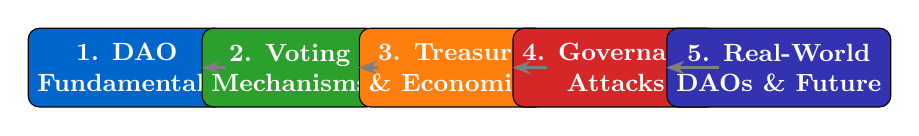
\begin{tikzpicture}[scale=0.9]
  \node[draw,fill=mlblue,text=white,rounded corners=4pt,
        minimum width=2.0cm,minimum height=1.0cm,align=center,font=\small\bfseries]
        (b1) at (0,0) {1. DAO\\Fundamentals};
  \node[draw,fill=mlgreen,text=white,rounded corners=4pt,
        minimum width=2.0cm,minimum height=1.0cm,align=center,font=\small\bfseries]
        (b2) at (2.3,0) {2. Voting\\Mechanisms};
  \node[draw,fill=mlorange,text=white,rounded corners=4pt,
        minimum width=2.0cm,minimum height=1.0cm,align=center,font=\small\bfseries]
        (b3) at (4.6,0) {3. Treasury\\\& Economics};
  \node[draw,fill=mlred,text=white,rounded corners=4pt,
        minimum width=2.0cm,minimum height=1.0cm,align=center,font=\small\bfseries]
        (b4) at (6.9,0) {4. Governance\\Attacks};
  \node[draw,fill=mlpurple,text=white,rounded corners=4pt,
        minimum width=2.0cm,minimum height=1.0cm,align=center,font=\small\bfseries]
        (b5) at (9.2,0) {5. Real-World\\DAOs \& Future};
  \draw[-{Stealth},thick,mlgray] (b1.east) -- (b2.west);
  \draw[-{Stealth},thick,mlgray] (b2.east) -- (b3.west);
  \draw[-{Stealth},thick,mlgray] (b3.east) -- (b4.west);
  \draw[-{Stealth},thick,mlgray] (b4.east) -- (b5.west);
\end{tikzpicture}
\vspace{3mm}

\column{0.45\textwidth}
\begin{block}{Learning Objectives}
\footnotesize
\begin{itemize}
  \item Understand DAO architecture and smart contract governance
  \item Analyse voting mechanisms from simple to advanced
  \item Evaluate treasury management and tokenomics
  \item Identify governance attack vectors and defences
  \item Assess real-world DAO case studies and future trends
\end{itemize}
\end{block}
\vspace{1mm}
\begin{block}{Prerequisites}
\footnotesize
\begin{itemize}
  \item Lessons 1--5: Blockchain fundamentals, smart contracts, DeFi
  \item Basic familiarity with ERC-20 tokens and Ethereum
\end{itemize}
\end{block}
\end{columns}
\bottomnote{Duration: 90 minutes | 5 sections | \textasciitilde55 frames | Prerequisite: Lessons 1--5}
\end{frame}

% Frame 3: Table of Contents
\begin{frame}{Table of Contents}
\tableofcontents
\bottomnote{Navigate through 5 sections covering DAO fundamentals to real-world governance and the future}
\end{frame}

\begin{frame}{Learning Objectives}
By the end of this lecture, you will be able to:
\begin{enumerate}
\item \textbf{Explain} DAO architecture and compare governance models (token, reputation, multisig)
\item \textbf{Analyze} voting mechanisms (quadratic voting, conviction voting, holographic consensus)
\item \textbf{Evaluate} treasury management strategies and token economic sustainability
\item \textbf{Identify} governance attack vectors (flash loan attacks, vote buying, Sybil attacks)
\item \textbf{Assess} real-world DAO governance through MakerDAO, Uniswap, and Aave case studies
\end{enumerate}
\bottomnote{Bloom's taxonomy levels: Remember $\rightarrow$ Understand $\rightarrow$ Apply $\rightarrow$ Analyze $\rightarrow$ Evaluate $\rightarrow$ Create}
\end{frame}

%% ============================================================
%% SECTION 1: DAO FUNDAMENTALS & ARCHITECTURE
%% ============================================================
\section{DAO Fundamentals \& Architecture}

% Frame 4: Section 1 Divider
\begin{frame}{}
\begin{beamercolorbox}[sep=12pt,center,rounded=true,shadow=true]{palette quaternary}
  {\Large\bfseries Section 1: DAO Fundamentals \& Architecture}\\[6pt]
  {\normalsize Understanding decentralized organizations and their smart contract foundations}
\end{beamercolorbox}
\vspace{4mm}
\begin{columns}[T]
\column{0.5\textwidth}
\begin{block}{What You Will Learn}
\footnotesize
\begin{itemize}
  \item What DAOs are and how they differ from traditional organizations
  \item Smart contract architecture for DAOs
  \item Membership models: token-based, share-based, reputation-based
  \item DAO creation frameworks and legal wrappers
\end{itemize}
\end{block}
\column{0.5\textwidth}
\begin{block}{Frames in This Section}
\footnotesize
\begin{itemize}
  \item Frame 5: What is a DAO?
  \item Frame 6: Traditional Organizations vs DAOs
  \item Frame 7: DAO Architecture Overview
  \item Frame 8: Governor Contract (Code)
  \item Frame 9: Membership Models
  \item Frame 10: Token-Based DAO Deep Dive
  \item Frame 11: DAO Creation Frameworks
  \item Frame 12: Legal Status of DAOs
  \item Frame 13: DAO Lifecycle
  \item Frame 14: Section 1 Summary
\end{itemize}
\end{block}
\end{columns}
\bottomnote{Section 1 of 5 | Frames 4--14}
\end{frame}

% Frame 5: What is a DAO?
\begin{frame}{What is a DAO?}
\begin{columns}[T]
\column{0.42\textwidth}
\begin{block}{Decentralized Autonomous Organization}
\footnotesize
\begin{itemize}
  \item \textbf{Organization encoded in smart contracts} -- rules are code, not documents
  \item \textbf{No central authority} -- no CEO, no board with unilateral power
  \item \textbf{Transparent and permissionless} -- anyone can read the code and participate
  \item \textbf{Governed by token holders} -- voting rights proportional to stake
  \item \textbf{Treasury on-chain} -- funds held collectively, disbursed by vote
\end{itemize}
\end{block}
\vspace{2mm}
\begin{exampleblock}{First DAO}
\footnotesize
``The DAO'' (2016) raised \$150M in ETH before being hacked via a reentrancy vulnerability -- leading to the Ethereum hard fork.
\end{exampleblock}

\column{0.58\textwidth}
\vspace{2mm}
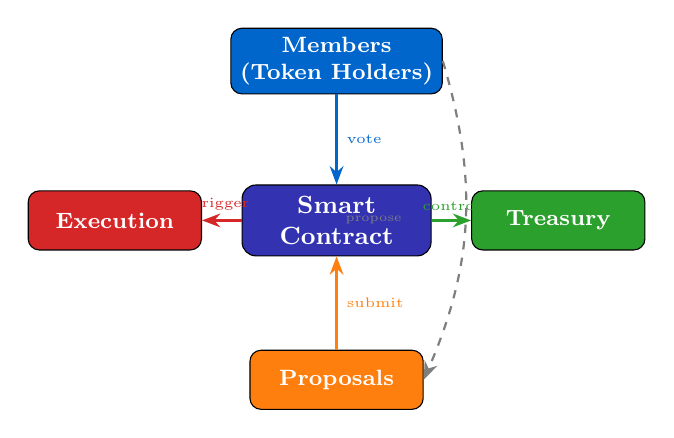
\begin{tikzpicture}[scale=0.88]
  % Central smart contract node
  \node[draw,fill=mlpurple,text=white,rounded corners=5pt,
        minimum width=2.4cm,minimum height=0.9cm,align=center,font=\small\bfseries]
        (sc) at (0,0) {Smart\\Contract};
  % Surrounding nodes
  \node[draw,fill=mlblue,text=white,rounded corners=4pt,
        minimum width=2.2cm,minimum height=0.75cm,align=center,font=\footnotesize\bfseries]
        (mem) at (0, 2.3) {Members\\(Token Holders)};
  \node[draw,fill=mlgreen,text=white,rounded corners=4pt,
        minimum width=2.2cm,minimum height=0.75cm,align=center,font=\footnotesize\bfseries]
        (treas) at (3.2, 0) {Treasury};
  \node[draw,fill=mlorange,text=white,rounded corners=4pt,
        minimum width=2.2cm,minimum height=0.75cm,align=center,font=\footnotesize\bfseries]
        (prop) at (0,-2.3) {Proposals};
  \node[draw,fill=mlred,text=white,rounded corners=4pt,
        minimum width=2.2cm,minimum height=0.75cm,align=center,font=\footnotesize\bfseries]
        (exec) at (-3.2, 0) {Execution};
  % Arrows
  \draw[-{Stealth},thick,mlblue] (mem.south) -- (sc.north)
        node[midway,right,font=\tiny,text=mlblue] {vote};
  \draw[-{Stealth},thick,mlgreen] (sc.east) -- (treas.west)
        node[midway,above,font=\tiny,text=mlgreen] {control};
  \draw[-{Stealth},thick,mlorange] (prop.north) -- (sc.south)
        node[midway,right,font=\tiny,text=mlorange] {submit};
  \draw[-{Stealth},thick,mlred] (sc.west) -- (exec.east)
        node[midway,above,font=\tiny,text=mlred] {trigger};
  \draw[-{Stealth},thick,mlgray,dashed] (mem.east) to[bend left=20] (prop.east)
        node[midway,right,font=\tiny,text=mlgray] {propose};
\end{tikzpicture}
\end{columns}
\bottomnote{DAOs replace legal contracts and corporate hierarchy with immutable code and token-based consensus}
\end{frame}

% Frame 6: Traditional Organizations vs DAOs
\begin{frame}{Traditional Organizations vs DAOs}
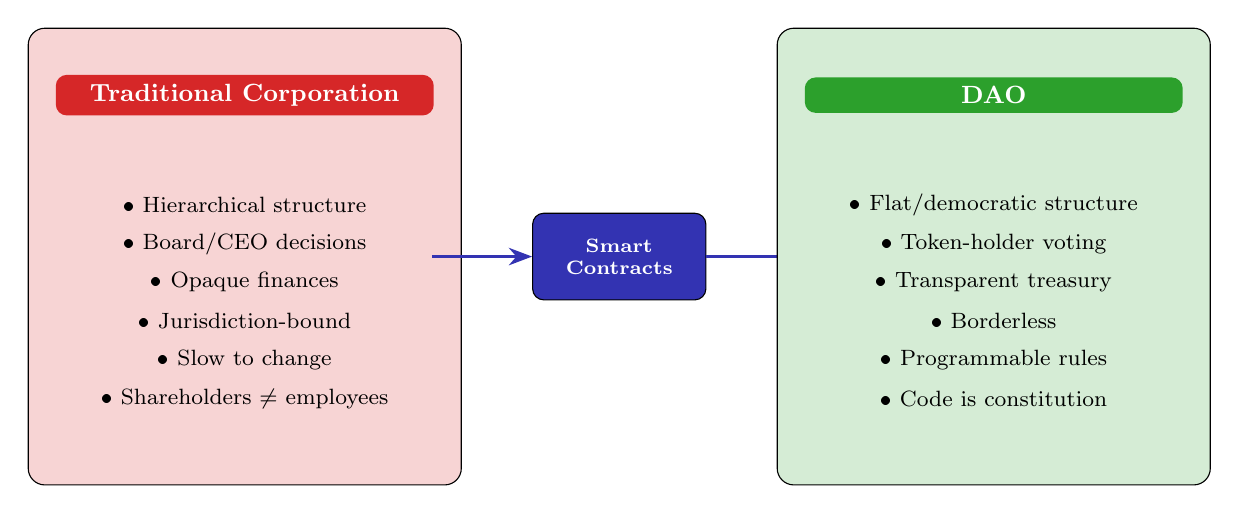
\begin{tikzpicture}[scale=0.82]
  % Left panel: Traditional Corp
  \node[draw,fill=mlred!20,rounded corners=6pt,
        minimum width=5.5cm,minimum height=5.8cm,align=center]
        (trad) at (0,0) {};
  \node[fill=mlred,text=white,rounded corners=4pt,font=\small\bfseries,
        minimum width=4.8cm,align=center]
        at (0,2.5) {Traditional Corporation};
  \node[font=\footnotesize,align=left,text=black] at (0,0.8)
        {\textbullet\ Hierarchical structure};
  \node[font=\footnotesize,align=left,text=black] at (0,0.2)
        {\textbullet\ Board/CEO decisions};
  \node[font=\footnotesize,align=left,text=black] at (0,-0.4)
        {\textbullet\ Opaque finances};
  \node[font=\footnotesize,align=left,text=black] at (0,-1.0)
        {\textbullet\ Jurisdiction-bound};
  \node[font=\footnotesize,align=left,text=black] at (0,-1.6)
        {\textbullet\ Slow to change};
  \node[font=\footnotesize,align=left,text=black] at (0,-2.2)
        {\textbullet\ Shareholders \(\neq\) employees};

  % Center: transformation arrow
  \node[draw,fill=mlpurple,text=white,rounded corners=4pt,
        font=\scriptsize\bfseries,align=center,
        minimum width=2.2cm,minimum height=1.1cm]
        (arr) at (5.8,0) {Smart\\Contracts};
  \draw[-{Stealth},very thick,mlpurple] (2.9,0) -- (arr.west);
  \draw[-{Stealth},very thick,mlpurple] (arr.east) -- (8.7,0);

  % Right panel: DAO
  \node[draw,fill=mlgreen!20,rounded corners=6pt,
        minimum width=5.5cm,minimum height=5.8cm,align=center]
        (dao) at (11.6,0) {};
  \node[fill=mlgreen,text=white,rounded corners=4pt,font=\small\bfseries,
        minimum width=4.8cm,align=center]
        at (11.6,2.5) {DAO};
  \node[font=\footnotesize,align=left,text=black] at (11.6,0.8)
        {\textbullet\ Flat/democratic structure};
  \node[font=\footnotesize,align=left,text=black] at (11.6,0.2)
        {\textbullet\ Token-holder voting};
  \node[font=\footnotesize,align=left,text=black] at (11.6,-0.4)
        {\textbullet\ Transparent treasury};
  \node[font=\footnotesize,align=left,text=black] at (11.6,-1.0)
        {\textbullet\ Borderless};
  \node[font=\footnotesize,align=left,text=black] at (11.6,-1.6)
        {\textbullet\ Programmable rules};
  \node[font=\footnotesize,align=left,text=black] at (11.6,-2.2)
        {\textbullet\ Code is constitution};
\end{tikzpicture}
\bottomnote{DAOs aim to replace trust in people with trust in code -- but code has its own risks}
\end{frame}

% Frame 7: DAO Architecture Overview
\begin{frame}{DAO Architecture Overview}
\centering
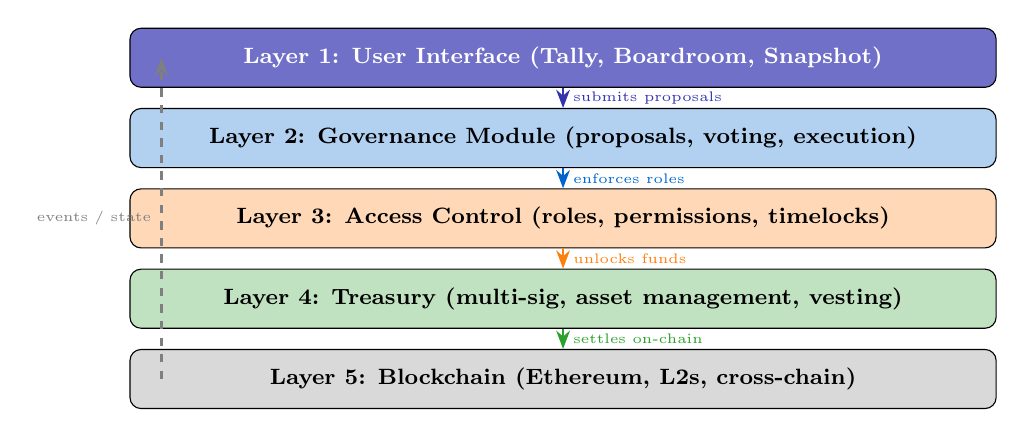
\begin{tikzpicture}[scale=0.85]
  % Layer 5: Blockchain (bottom)
  \node[draw,fill=mlgray!30,rounded corners=4pt,
        minimum width=11cm,minimum height=0.75cm,align=center,font=\footnotesize\bfseries]
        (l5) at (0,-3.6) {Layer 5: Blockchain (Ethereum, L2s, cross-chain)};
  % Layer 4: Treasury
  \node[draw,fill=mlgreen!30,rounded corners=4pt,
        minimum width=11cm,minimum height=0.75cm,align=center,font=\footnotesize\bfseries]
        (l4) at (0,-2.4) {Layer 4: Treasury (multi-sig, asset management, vesting)};
  % Layer 3: Access Control
  \node[draw,fill=mlorange!30,rounded corners=4pt,
        minimum width=11cm,minimum height=0.75cm,align=center,font=\footnotesize\bfseries]
        (l3) at (0,-1.2) {Layer 3: Access Control (roles, permissions, timelocks)};
  % Layer 2: Governance Module
  \node[draw,fill=mlblue!30,rounded corners=4pt,
        minimum width=11cm,minimum height=0.75cm,align=center,font=\footnotesize\bfseries]
        (l2) at (0,0) {Layer 2: Governance Module (proposals, voting, execution)};
  % Layer 1: UI (top)
  \node[draw,fill=mlpurple!70,text=white,rounded corners=4pt,
        minimum width=11cm,minimum height=0.75cm,align=center,font=\footnotesize\bfseries]
        (l1) at (0,1.2) {Layer 1: User Interface (Tally, Boardroom, Snapshot)};

  % Vertical arrows (interaction flows)
  \draw[-{Stealth},thick,mlpurple] (l1.south) -- (l2.north)
        node[midway,right,font=\tiny] {submits proposals};
  \draw[-{Stealth},thick,mlblue] (l2.south) -- (l3.north)
        node[midway,right,font=\tiny] {enforces roles};
  \draw[-{Stealth},thick,mlorange] (l3.south) -- (l4.north)
        node[midway,right,font=\tiny] {unlocks funds};
  \draw[-{Stealth},thick,mlgreen] (l4.south) -- (l5.north)
        node[midway,right,font=\tiny] {settles on-chain};

  % Feedback arrow
  \draw[-{Stealth},thick,mlgray,dashed] (-6.0,-3.6) -- (-6.0,1.2)
        node[midway,left,font=\tiny,text=mlgray] {events / state};
\end{tikzpicture}
\bottomnote{OpenZeppelin Governor is the dominant Layer 2 implementation; Gnosis Safe dominates Layer 4 treasury management}
\end{frame}

% Frame 8: Governor Contract Architecture [FRAGILE] -- CODE FRAME 1
\begin{frame}[fragile]{Governor Contract Architecture}
\begin{columns}[T]
\column{0.55\textwidth}
\begin{lstlisting}[language=Solidity,basicstyle=\ttfamily\tiny,
  caption={Simplified Governor Contract}]
// Simplified Governor Contract
contract DAOGovernor {
    uint256 public proposalCount;
    uint256 public quorumVotes;
    uint256 public votingPeriod;

    struct Proposal {
        address proposer;
        uint256 forVotes;
        uint256 againstVotes;
        uint256 endBlock;
        bool executed;
    }

    mapping(uint256 => Proposal)
        public proposals;

    function propose(
        string memory description
    ) external returns (uint256) {
        proposalCount++;
        proposals[proposalCount] =
            Proposal(msg.sender,
                0, 0,
                block.number + votingPeriod,
                false);
        return proposalCount;
    }
}
\end{lstlisting}

\column{0.45\textwidth}
\vspace{2mm}
\begin{block}{Governor Architecture}
\footnotesize
\begin{itemize}
  \item \textbf{Proposal struct} stores proposer, vote tallies, deadline block, and execution status
  \item \textbf{proposalCount} acts as auto-incrementing ID and prevents hash collisions
  \item \textbf{votingPeriod} is measured in blocks ($\approx$12s on mainnet), typically 40,320 blocks = 7 days
  \item \textbf{quorumVotes} sets minimum participation threshold to prevent low-turnout attacks
\end{itemize}
\end{block}
\vspace{2mm}
\begin{exampleblock}{Production Standard}
\footnotesize
OpenZeppelin Governor (OZ) extends this pattern with:
\begin{itemize}
  \item ERC20Votes checkpointing for snapshot-based voting power
  \item Timelock controller for delayed execution
  \item Modular extensions (Bravo-compatible, fractional voting)
\end{itemize}
\end{exampleblock}
\end{columns}
\bottomnote{OpenZeppelin Governor is used by Compound, Uniswap, and most major DAOs -- always audit before deployment}
\end{frame}

% Frame 9: Membership Models
\begin{frame}{Membership Models}
\vspace{-1mm}
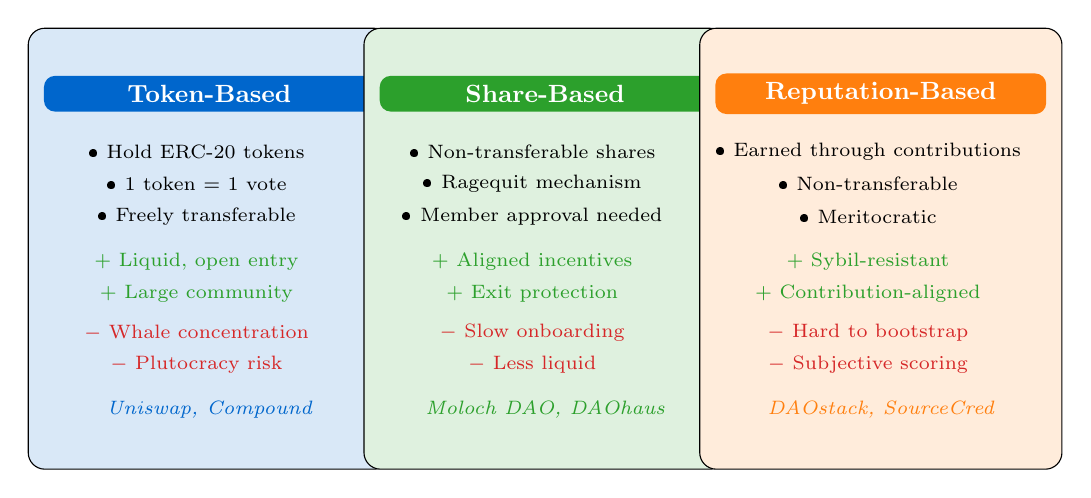
\begin{tikzpicture}[scale=0.82]
  %% Panel 1: Token-Based (mlblue)
  \node[draw,fill=mlblue!15,rounded corners=6pt,
        minimum width=4.6cm,minimum height=5.6cm]
        at (0,0) {};
  \node[fill=mlblue,text=white,rounded corners=4pt,font=\small\bfseries,
        minimum width=4.2cm,align=center]
        at (0,2.4) {Token-Based};
  \node[font=\scriptsize,align=left] at (-0.2,1.5)
        {\textbullet\ Hold ERC-20 tokens};
  \node[font=\scriptsize,align=left] at (-0.2,1.0)
        {\textbullet\ 1 token = 1 vote};
  \node[font=\scriptsize,align=left] at (-0.2,0.5)
        {\textbullet\ Freely transferable};
  \node[font=\scriptsize,align=left,text=mlgreen] at (-0.2,-0.2)
        {\(+\) Liquid, open entry};
  \node[font=\scriptsize,align=left,text=mlgreen] at (-0.2,-0.7)
        {\(+\) Large community};
  \node[font=\scriptsize,align=left,text=mlred] at (-0.2,-1.3)
        {\(-\) Whale concentration};
  \node[font=\scriptsize,align=left,text=mlred] at (-0.2,-1.8)
        {\(-\) Plutocracy risk};
  \node[font=\scriptsize,align=center,text=mlblue,font=\scriptsize\itshape]
        at (0,-2.5) {Uniswap, Compound};

  %% Panel 2: Share-Based (mlgreen)
  \node[draw,fill=mlgreen!15,rounded corners=6pt,
        minimum width=4.6cm,minimum height=5.6cm]
        at (5.2,0) {};
  \node[fill=mlgreen,text=white,rounded corners=4pt,font=\small\bfseries,
        minimum width=4.2cm,align=center]
        at (5.2,2.4) {Share-Based};
  \node[font=\scriptsize,align=left] at (5.0,1.5)
        {\textbullet\ Non-transferable shares};
  \node[font=\scriptsize,align=left] at (5.0,1.0)
        {\textbullet\ Ragequit mechanism};
  \node[font=\scriptsize,align=left] at (5.0,0.5)
        {\textbullet\ Member approval needed};
  \node[font=\scriptsize,align=left,text=mlgreen] at (5.0,-0.2)
        {\(+\) Aligned incentives};
  \node[font=\scriptsize,align=left,text=mlgreen] at (5.0,-0.7)
        {\(+\) Exit protection};
  \node[font=\scriptsize,align=left,text=mlred] at (5.0,-1.3)
        {\(-\) Slow onboarding};
  \node[font=\scriptsize,align=left,text=mlred] at (5.0,-1.8)
        {\(-\) Less liquid};
  \node[font=\scriptsize,align=center,text=mlgreen,font=\scriptsize\itshape]
        at (5.2,-2.5) {Moloch DAO, DAOhaus};

  %% Panel 3: Reputation-Based (mlorange)
  \node[draw,fill=mlorange!15,rounded corners=6pt,
        minimum width=4.6cm,minimum height=5.6cm]
        at (10.4,0) {};
  \node[fill=mlorange,text=white,rounded corners=4pt,font=\small\bfseries,
        minimum width=4.2cm,align=center]
        at (10.4,2.4) {Reputation-Based};
  \node[font=\scriptsize,align=left] at (10.2,1.5)
        {\textbullet\ Earned through contributions};
  \node[font=\scriptsize,align=left] at (10.2,1.0)
        {\textbullet\ Non-transferable};
  \node[font=\scriptsize,align=left] at (10.2,0.5)
        {\textbullet\ Meritocratic};
  \node[font=\scriptsize,align=left,text=mlgreen] at (10.2,-0.2)
        {\(+\) Sybil-resistant};
  \node[font=\scriptsize,align=left,text=mlgreen] at (10.2,-0.7)
        {\(+\) Contribution-aligned};
  \node[font=\scriptsize,align=left,text=mlred] at (10.2,-1.3)
        {\(-\) Hard to bootstrap};
  \node[font=\scriptsize,align=left,text=mlred] at (10.2,-1.8)
        {\(-\) Subjective scoring};
  \node[font=\scriptsize,align=center,text=mlorange,font=\scriptsize\itshape]
        at (10.4,-2.5) {DAOstack, SourceCred};
\end{tikzpicture}
\bottomnote{Most real-world DAOs use token-based governance due to simplicity, but share-based models offer stronger alignment}
\end{frame}

% Frame 10: Token-Based DAO Deep Dive
\begin{frame}{Token-Based DAO Deep Dive}
\begin{columns}[T]
\column{0.50\textwidth}
\begin{block}{Mechanics of Token Governance}
\footnotesize
\begin{itemize}
  \item \textbf{Token distribution} determines governance power from day one -- initial allocation is a political act
  \item \textbf{Delegation}: holders can delegate voting power to active participants without transferring tokens (ERC20Votes)
  \item \textbf{Whale concentration}: top 10 addresses in many DAOs control $>$50\% of votes
  \item \textbf{Governance Extractable Value (GEV)}: large holders can profit by passing self-serving proposals
  \item \textbf{Voter apathy}: typical participation rates are 5--15\% of circulating supply
\end{itemize}
\end{block}
\vspace{2mm}
\begin{alertblock}{Plutocracy Problem}
\footnotesize
1 token = 1 vote \(\Rightarrow\) wealthiest wallets dominate. Quadratic voting and conviction voting (Section 2) address this.
\end{alertblock}

\column{0.50\textwidth}
\vspace{2mm}
\begin{center}
\textbf{\small Typical Governance Token Distribution}
\end{center}
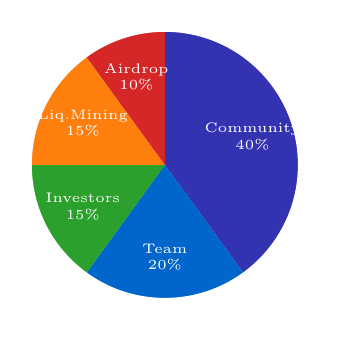
\begin{tikzpicture}[scale=0.78]
  % Approximate pie chart using arcs
  % Team 20%, Investors 15%, Community Treasury 40%, Liquidity Mining 15%, Airdrop 10%
  % Using bar chart instead for TikZ simplicity without \foreach multi-var
  \begin{scope}
    % Community Treasury 40% (mlpurple)
    \fill[mlpurple] (0,0) -- (90:2.2cm) arc(90:-54:2.2cm) -- cycle;
    % Team 20% (mlblue)
    \fill[mlblue] (0,0) -- (-54:2.2cm) arc(-54:-126:2.2cm) -- cycle;
    % Investors 15% (mlgreen)
    \fill[mlgreen] (0,0) -- (-126:2.2cm) arc(-126:-180:2.2cm) -- cycle;
    % Liquidity Mining 15% (mlorange)
    \fill[mlorange] (0,0) -- (180:2.2cm) arc(180:126:2.2cm) -- cycle;
    % Airdrop 10% (mlred)
    \fill[mlred] (0,0) -- (126:2.2cm) arc(126:90:2.2cm) -- cycle;
    \draw[white,line width=1.5pt] (0,0) circle(2.2cm);
  \end{scope}
  % Labels
  \node[font=\tiny,text=white,align=center] at (18:1.5cm) {Community\\40\%};
  \node[font=\tiny,text=white,align=center] at (-90:1.5cm) {Team\\20\%};
  \node[font=\tiny,text=white,align=center] at (-153:1.5cm) {Investors\\15\%};
  \node[font=\tiny,text=white,align=center] at (153:1.5cm) {Liq.Mining\\15\%};
  \node[font=\tiny,text=white,align=center] at (108:1.5cm) {Airdrop\\10\%};
\end{tikzpicture}
\vspace{1mm}
\footnotesize\textit{Token distribution = governance power distribution}
\end{columns}
\bottomnote{Uniswap: top 10 delegates control \textasciitilde70\% of votes; voter participation peaked at \textasciitilde40M UNI in early proposals}
\end{frame}

% Frame 11: DAO Creation Frameworks
\begin{frame}{DAO Creation Frameworks}
\vspace{-1mm}
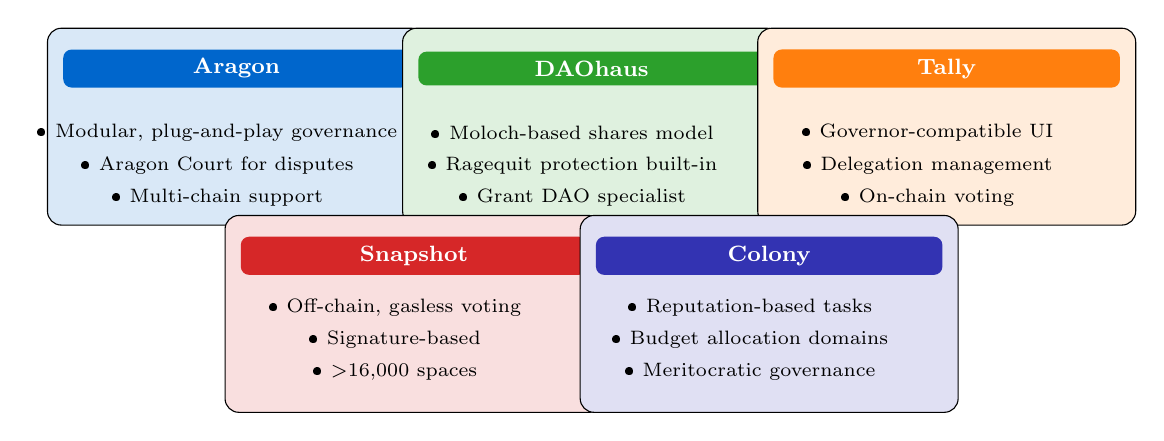
\begin{tikzpicture}[scale=0.82]
  %% Aragon (top-left)
  \node[draw,fill=mlblue!15,rounded corners=5pt,
        minimum width=4.8cm,minimum height=2.5cm,align=center]
        (aragon) at (0,2.6) {};
  \node[fill=mlblue,text=white,rounded corners=3pt,font=\footnotesize\bfseries,
        minimum width=4.4cm,align=center] at (0,3.5) {Aragon};
  \node[font=\scriptsize,align=left] at (-0.3,2.5)
        {\textbullet\ Modular, plug-and-play governance};
  \node[font=\scriptsize,align=left] at (-0.3,2.0)
        {\textbullet\ Aragon Court for disputes};
  \node[font=\scriptsize,align=left] at (-0.3,1.5)
        {\textbullet\ Multi-chain support};

  %% DAOhaus (top-right)
  \node[draw,fill=mlgreen!15,rounded corners=5pt,
        minimum width=4.8cm,minimum height=2.5cm,align=center]
        (daohaus) at (5.5,2.6) {};
  \node[fill=mlgreen,text=white,rounded corners=3pt,font=\footnotesize\bfseries,
        minimum width=4.4cm,align=center] at (5.5,3.5) {DAOhaus};
  \node[font=\scriptsize,align=left] at (5.2,2.5)
        {\textbullet\ Moloch-based shares model};
  \node[font=\scriptsize,align=left] at (5.2,2.0)
        {\textbullet\ Ragequit protection built-in};
  \node[font=\scriptsize,align=left] at (5.2,1.5)
        {\textbullet\ Grant DAO specialist};

  %% Tally (top-far-right)
  \node[draw,fill=mlorange!15,rounded corners=5pt,
        minimum width=4.8cm,minimum height=2.5cm,align=center]
        (tally) at (11.0,2.6) {};
  \node[fill=mlorange,text=white,rounded corners=3pt,font=\footnotesize\bfseries,
        minimum width=4.4cm,align=center] at (11.0,3.5) {Tally};
  \node[font=\scriptsize,align=left] at (10.7,2.5)
        {\textbullet\ Governor-compatible UI};
  \node[font=\scriptsize,align=left] at (10.7,2.0)
        {\textbullet\ Delegation management};
  \node[font=\scriptsize,align=left] at (10.7,1.5)
        {\textbullet\ On-chain voting};

  %% Snapshot (bottom-left)
  \node[draw,fill=mlred!15,rounded corners=5pt,
        minimum width=4.8cm,minimum height=2.5cm,align=center]
        (snap) at (2.75,-0.3) {};
  \node[fill=mlred,text=white,rounded corners=3pt,font=\footnotesize\bfseries,
        minimum width=4.4cm,align=center] at (2.75,0.6) {Snapshot};
  \node[font=\scriptsize,align=left] at (2.45,-0.2)
        {\textbullet\ Off-chain, gasless voting};
  \node[font=\scriptsize,align=left] at (2.45,-0.7)
        {\textbullet\ Signature-based};
  \node[font=\scriptsize,align=left] at (2.45,-1.2)
        {\textbullet\ \textgreater 16,000 spaces};

  %% Colony (bottom-right)
  \node[draw,fill=mlpurple!15,rounded corners=5pt,
        minimum width=4.8cm,minimum height=2.5cm,align=center]
        (colony) at (8.25,-0.3) {};
  \node[fill=mlpurple,text=white,rounded corners=3pt,font=\footnotesize\bfseries,
        minimum width=4.4cm,align=center] at (8.25,0.6) {Colony};
  \node[font=\scriptsize,align=left] at (7.95,-0.2)
        {\textbullet\ Reputation-based tasks};
  \node[font=\scriptsize,align=left] at (7.95,-0.7)
        {\textbullet\ Budget allocation domains};
  \node[font=\scriptsize,align=left] at (7.95,-1.2)
        {\textbullet\ Meritocratic governance};
\end{tikzpicture}
\bottomnote{Snapshot + Tally is the most common hybrid: gasless signalling on Snapshot, binding execution via on-chain Governor}
\end{frame}

% Frame 12: Legal Status of DAOs
\begin{frame}{Legal Status of DAOs}
\begin{columns}[T]
\column{0.52\textwidth}
\vspace{1mm}
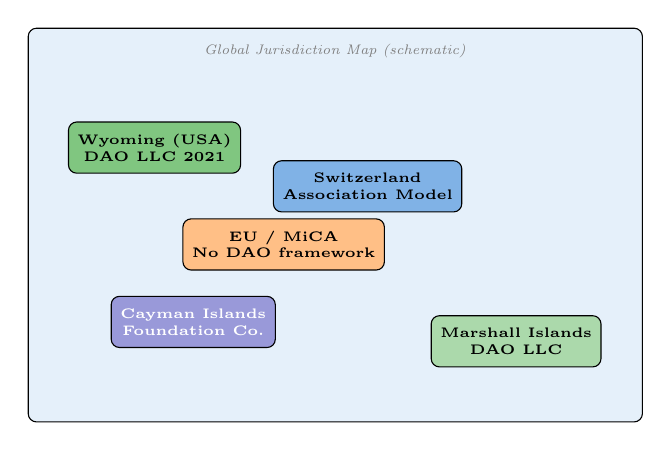
\begin{tikzpicture}[scale=0.82]
  % World map schematic (simplified rectangle regions)
  \node[draw,fill=mlblue!10,rounded corners=3pt,
        minimum width=7.8cm,minimum height=5.0cm] at (0,0) {};
  \node[font=\tiny,text=mlgray] at (0,2.7) {\textit{Global Jurisdiction Map (schematic)}};

  % USA / Wyoming
  \node[draw,fill=mlgreen!60,rounded corners=3pt,font=\tiny\bfseries,
        minimum width=2.0cm,minimum height=0.65cm,align=center]
        at (-2.8,1.2) {Wyoming (USA)\\DAO LLC 2021};
  % Marshall Islands
  \node[draw,fill=mlgreen!40,rounded corners=3pt,font=\tiny\bfseries,
        minimum width=2.0cm,minimum height=0.65cm,align=center]
        at (2.8,-1.8) {Marshall Islands\\DAO LLC};
  % Switzerland
  \node[draw,fill=mlblue!50,rounded corners=3pt,font=\tiny\bfseries,
        minimum width=2.0cm,minimum height=0.65cm,align=center]
        at (0.5,0.6) {Switzerland\\Association Model};
  % EU / MiCA
  \node[draw,fill=mlorange!50,rounded corners=3pt,font=\tiny\bfseries,
        minimum width=2.0cm,minimum height=0.65cm,align=center]
        at (-0.8,-0.3) {EU / MiCA\\No DAO framework};
  % Cayman Islands
  \node[draw,fill=mlpurple!50,text=white,rounded corners=3pt,font=\tiny\bfseries,
        minimum width=2.0cm,minimum height=0.65cm,align=center]
        at (-2.2,-1.5) {Cayman Islands\\Foundation Co.};
\end{tikzpicture}

\column{0.48\textwidth}
\begin{block}{Legal Wrapper Concept}
\footnotesize
\textbf{DAO + Legal Entity = }
\begin{itemize}
  \item Limited liability for members
  \item Ability to sign contracts
  \item Bank accounts and payroll
  \item Regulatory compliance
  \item IP ownership
\end{itemize}
\end{block}
\vspace{2mm}
\begin{alertblock}{Unresolved Issues}
\footnotesize
\begin{itemize}
  \item Who is liable when a DAO is hacked?
  \item Are token holders employees or partners?
  \item Tax treatment varies by jurisdiction
  \item Securities law: is a governance token a security?
\end{itemize}
\end{alertblock}
\end{columns}
\bottomnote{Legal wrapping is essential for DAOs interacting with the traditional world -- contracts, bank accounts, and liability protection}
\end{frame}

% Frame 13: DAO Lifecycle
\begin{frame}{DAO Lifecycle}
\vspace{2mm}
\centering
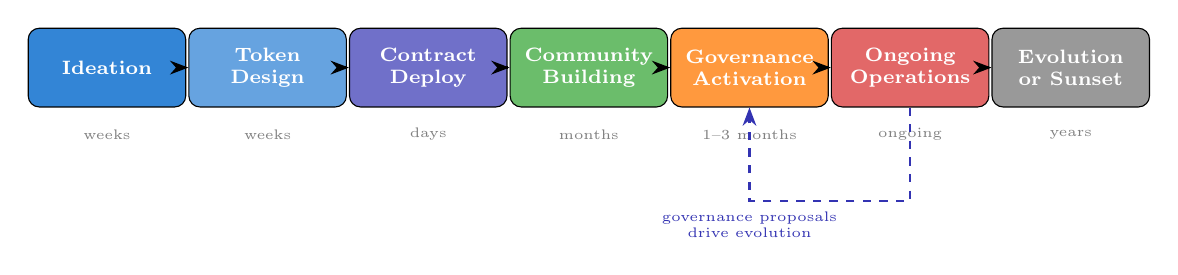
\begin{tikzpicture}[scale=0.85,node distance=0cm]
  % Lifecycle nodes (horizontal chain)
  \node[draw,fill=mlblue!80,text=white,rounded corners=4pt,
        minimum width=2.0cm,minimum height=1.0cm,align=center,font=\scriptsize\bfseries]
        (n1) at (0,0) {Ideation};
  \node[draw,fill=mlblue!60,text=white,rounded corners=4pt,
        minimum width=2.0cm,minimum height=1.0cm,align=center,font=\scriptsize\bfseries]
        (n2) at (2.4,0) {Token\\Design};
  \node[draw,fill=mlpurple!70,text=white,rounded corners=4pt,
        minimum width=2.0cm,minimum height=1.0cm,align=center,font=\scriptsize\bfseries]
        (n3) at (4.8,0) {Contract\\Deploy};
  \node[draw,fill=mlgreen!70,text=white,rounded corners=4pt,
        minimum width=2.0cm,minimum height=1.0cm,align=center,font=\scriptsize\bfseries]
        (n4) at (7.2,0) {Community\\Building};
  \node[draw,fill=mlorange!80,text=white,rounded corners=4pt,
        minimum width=2.0cm,minimum height=1.0cm,align=center,font=\scriptsize\bfseries]
        (n5) at (9.6,0) {Governance\\Activation};
  \node[draw,fill=mlred!70,text=white,rounded corners=4pt,
        minimum width=2.0cm,minimum height=1.0cm,align=center,font=\scriptsize\bfseries]
        (n6) at (12.0,0) {Ongoing\\Operations};
  \node[draw,fill=mlgray!80,text=white,rounded corners=4pt,
        minimum width=2.0cm,minimum height=1.0cm,align=center,font=\scriptsize\bfseries]
        (n7) at (14.4,0) {Evolution\\or Sunset};

  % Forward arrows
  \draw[-{Stealth},thick] (n1.east) -- (n2.west);
  \draw[-{Stealth},thick] (n2.east) -- (n3.west);
  \draw[-{Stealth},thick] (n3.east) -- (n4.west);
  \draw[-{Stealth},thick] (n4.east) -- (n5.west);
  \draw[-{Stealth},thick] (n5.east) -- (n6.west);
  \draw[-{Stealth},thick] (n6.east) -- (n7.west);

  % Time annotations below
  \node[font=\tiny,text=mlgray,align=center] at (0,-1.0) {weeks};
  \node[font=\tiny,text=mlgray,align=center] at (2.4,-1.0) {weeks};
  \node[font=\tiny,text=mlgray,align=center] at (4.8,-1.0) {days};
  \node[font=\tiny,text=mlgray,align=center] at (7.2,-1.0) {months};
  \node[font=\tiny,text=mlgray,align=center] at (9.6,-1.0) {1--3 months};
  \node[font=\tiny,text=mlgray,align=center] at (12.0,-1.0) {ongoing};
  \node[font=\tiny,text=mlgray,align=center] at (14.4,-1.0) {years};

  % Feedback loop: Operations -> Governance Activation
  \draw[-{Stealth},thick,mlpurple,dashed]
        (n6.south) -- ++(0,-1.4) -| (n5.south)
        node[midway,below,font=\tiny,text=mlpurple,align=center] {governance proposals\\drive evolution};
\end{tikzpicture}
\vspace{3mm}
\begin{columns}[T]
\column{0.33\textwidth}
\begin{block}{\footnotesize Launch Risks}
\scriptsize
\begin{itemize}
  \item Unaudited contracts
  \item Uneven token distribution
  \item Premature decentralization
\end{itemize}
\end{block}
\column{0.33\textwidth}
\begin{block}{\footnotesize Growth Challenges}
\scriptsize
\begin{itemize}
  \item Voter apathy
  \item Contributor retention
  \item Treasury runway
\end{itemize}
\end{block}
\column{0.33\textwidth}
\begin{block}{\footnotesize Exit Scenarios}
\scriptsize
\begin{itemize}
  \item Protocol ossification
  \item Acquisition by another DAO
  \item Graceful wind-down
\end{itemize}
\end{block}
\end{columns}
\bottomnote{Most DAOs fail within 2 years due to voter apathy and treasury mismanagement -- lifecycle planning is critical}
\end{frame}

% Frame 14: Section 1 Summary
\begin{frame}{Section 1 Summary: DAO Fundamentals}
\vspace{2mm}
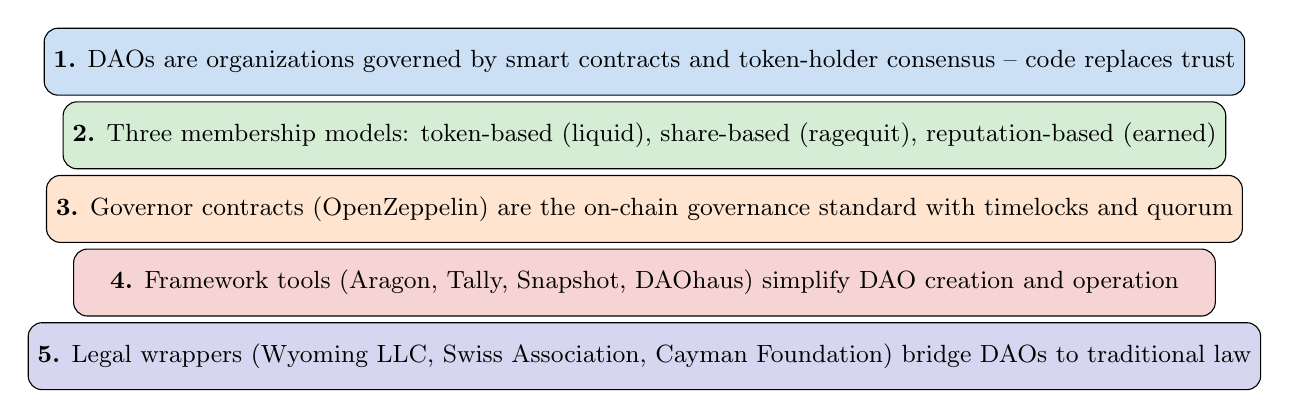
\begin{tikzpicture}[scale=0.85]
  % Box 1
  \node[draw,fill=mlblue!20,rounded corners=5pt,
        minimum width=14.5cm,minimum height=0.85cm,align=center,font=\small]
        at (0, 2.4) {\textbf{1.} DAOs are organizations governed by smart contracts and token-holder consensus -- code replaces trust};
  % Box 2
  \node[draw,fill=mlgreen!20,rounded corners=5pt,
        minimum width=14.5cm,minimum height=0.85cm,align=center,font=\small]
        at (0, 1.3) {\textbf{2.} Three membership models: token-based (liquid), share-based (ragequit), reputation-based (earned)};
  % Box 3
  \node[draw,fill=mlorange!20,rounded corners=5pt,
        minimum width=14.5cm,minimum height=0.85cm,align=center,font=\small]
        at (0, 0.2) {\textbf{3.} Governor contracts (OpenZeppelin) are the on-chain governance standard with timelocks and quorum};
  % Box 4
  \node[draw,fill=mlred!20,rounded corners=5pt,
        minimum width=14.5cm,minimum height=0.85cm,align=center,font=\small]
        at (0,-0.9) {\textbf{4.} Framework tools (Aragon, Tally, Snapshot, DAOhaus) simplify DAO creation and operation};
  % Box 5
  \node[draw,fill=mlpurple!20,rounded corners=5pt,
        minimum width=14.5cm,minimum height=0.85cm,align=center,font=\small]
        at (0,-2.0) {\textbf{5.} Legal wrappers (Wyoming LLC, Swiss Association, Cayman Foundation) bridge DAOs to traditional law};
\end{tikzpicture}
\vspace{4mm}
\begin{center}
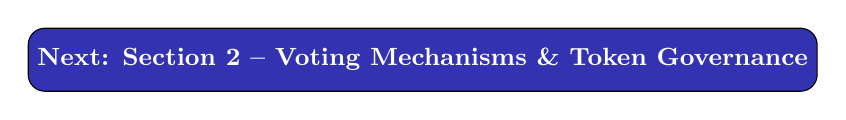
\begin{tikzpicture}
  \node[draw,fill=mlpurple,text=white,rounded corners=6pt,
        minimum width=10cm,minimum height=0.8cm,align=center,font=\small\bfseries]
        at (0,0) {Next: Section 2 -- Voting Mechanisms \& Token Governance};
\end{tikzpicture}
\end{center}
\bottomnote{Section 1 complete | Key insight: DAOs encode organizational rules as immutable (or upgradeable) smart contracts}
\end{frame}

%% ============================================================
%% SECTION 2: VOTING MECHANISMS & TOKEN GOVERNANCE
%% ============================================================
\section{Voting Mechanisms \& Token Governance}

% Frame 15: Section 2 Divider
\begin{frame}{}
\begin{beamercolorbox}[sep=12pt,center,rounded=true,shadow=true]{palette quaternary}
  {\Large\bfseries Section 2: Voting Mechanisms \& Token Governance}\\[6pt]
  {\normalsize How decentralized decisions get made -- from simple voting to advanced mechanisms}
\end{beamercolorbox}
\vspace{4mm}
\begin{columns}[T]
\column{0.5\textwidth}
\begin{block}{What You Will Learn}
\footnotesize
\begin{itemize}
  \item On-chain vs off-chain voting tradeoffs
  \item Token-weighted voting and its plutocracy problem
  \item Advanced mechanisms: quadratic, conviction, holographic consensus
  \item Delegation, timelocks, and proposal lifecycle
\end{itemize}
\end{block}
\column{0.5\textwidth}
\begin{block}{Frames in This Section}
\footnotesize
\begin{itemize}
  \item Frame 16: Proposal Lifecycle
  \item Frame 17: On-Chain vs Off-Chain Voting
  \item Frame 18: On-Chain Voting Power (Code)
  \item Frame 19: Simple Token Voting
  \item Frame 20: Quadratic Voting
  \item Frame 21: Conviction Voting
  \item Frame 22: Vote Delegation
  \item Frame 23: Quorum and Thresholds
  \item Frame 24: Holographic Consensus
  \item Frame 25: Timelocks and Execution
  \item Frame 26: Section 2 Summary
\end{itemize}
\end{block}
\end{columns}
\bottomnote{Section 2 of 5 | Frames 15--26}
\end{frame}

% Frame 16: Proposal Lifecycle
\begin{frame}{Proposal Lifecycle}
\vspace{1mm}
\centering
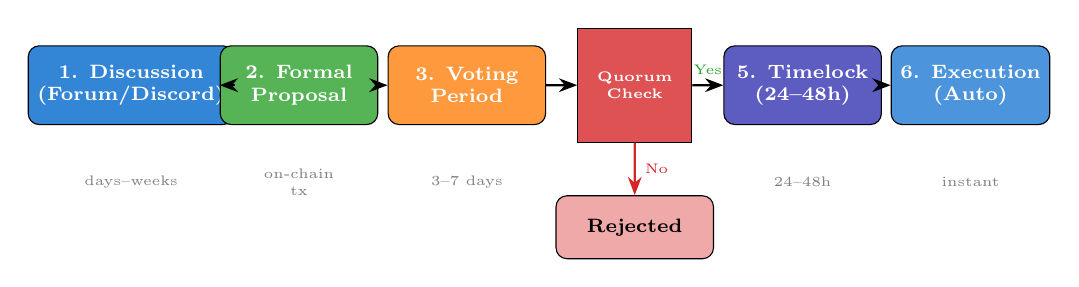
\begin{tikzpicture}[scale=0.82]
  %% Stage boxes (horizontal flow)
  \node[draw,fill=mlblue!80,text=white,rounded corners=4pt,
        minimum width=2.0cm,minimum height=1.0cm,align=center,font=\scriptsize\bfseries]
        (s1) at (0,0) {1. Discussion\\(Forum/Discord)};
  \node[draw,fill=mlgreen!80,text=white,rounded corners=4pt,
        minimum width=2.0cm,minimum height=1.0cm,align=center,font=\scriptsize\bfseries]
        (s2) at (2.6,0) {2. Formal\\Proposal};
  \node[draw,fill=mlorange!80,text=white,rounded corners=4pt,
        minimum width=2.0cm,minimum height=1.0cm,align=center,font=\scriptsize\bfseries]
        (s3) at (5.2,0) {3. Voting\\Period};
  %% Decision diamond at quorum check
  \node[draw,fill=mlred!80,text=white,regular polygon,regular polygon sides=4,
        minimum width=1.5cm,minimum height=1.5cm,align=center,font=\tiny\bfseries,
        inner sep=1pt]
        (s4) at (7.8,0) {Quorum\\Check};
  \node[draw,fill=mlpurple!80,text=white,rounded corners=4pt,
        minimum width=2.0cm,minimum height=1.0cm,align=center,font=\scriptsize\bfseries]
        (s5) at (10.4,0) {5. Timelock\\(24--48h)};
  \node[draw,fill=mlblue!70,text=white,rounded corners=4pt,
        minimum width=2.0cm,minimum height=1.0cm,align=center,font=\scriptsize\bfseries]
        (s6) at (13.0,0) {6. Execution\\(Auto)};
  %% Rejected node
  \node[draw,fill=mlred!40,rounded corners=4pt,
        minimum width=2.0cm,minimum height=0.8cm,align=center,font=\scriptsize\bfseries]
        (rej) at (7.8,-2.2) {Rejected};

  %% Flow arrows
  \draw[-{Stealth},thick] (s1.east) -- (s2.west);
  \draw[-{Stealth},thick] (s2.east) -- (s3.west);
  \draw[-{Stealth},thick] (s3.east) -- (s4.west);
  \draw[-{Stealth},thick] (s4.east) -- (s5.west)
        node[midway,above,font=\tiny,text=mlgreen] {Yes};
  \draw[-{Stealth},thick] (s5.east) -- (s6.west);
  \draw[-{Stealth},thick,mlred] (s4.south) -- (rej.north)
        node[midway,right,font=\tiny,text=mlred] {No};

  %% Time annotations below main flow
  \node[font=\tiny,text=mlgray,align=center] at (0,-1.5) {days--weeks};
  \node[font=\tiny,text=mlgray,align=center] at (2.6,-1.5) {on-chain\\tx};
  \node[font=\tiny,text=mlgray,align=center] at (5.2,-1.5) {3--7 days};
  \node[font=\tiny,text=mlgray,align=center] at (10.4,-1.5) {24--48h};
  \node[font=\tiny,text=mlgray,align=center] at (13.0,-1.5) {instant};
\end{tikzpicture}
\begin{columns}[T]
\column{0.33\textwidth}
\begin{block}{\footnotesize Stage Details}
\scriptsize
\begin{itemize}
  \item \textbf{Discussion}: Governance forums (Discourse, Commonwealth), temperature checks
  \item \textbf{Proposal}: Proposer must hold minimum tokens (e.g., 1M UNI to propose on Uniswap)
\end{itemize}
\end{block}
\column{0.33\textwidth}
\begin{block}{\footnotesize Voting Details}
\scriptsize
\begin{itemize}
  \item For/Against/Abstain votes accumulated over block range
  \item Snapshot of voting power taken at proposal block
  \item Prevents last-minute token purchases for votes
\end{itemize}
\end{block}
\column{0.33\textwidth}
\begin{block}{\footnotesize Execution}
\scriptsize
\begin{itemize}
  \item TimelockController queues transactions
  \item Anyone can trigger execution after delay
  \item On-chain atomicity: all-or-nothing
\end{itemize}
\end{block}
\end{columns}
\bottomnote{The full lifecycle from idea to on-chain execution typically takes 2--4 weeks -- deliberate slowness is a security feature}
\end{frame}

% Frame 17: On-Chain vs Off-Chain Voting
\begin{frame}{On-Chain vs Off-Chain Voting}
\vspace{1mm}
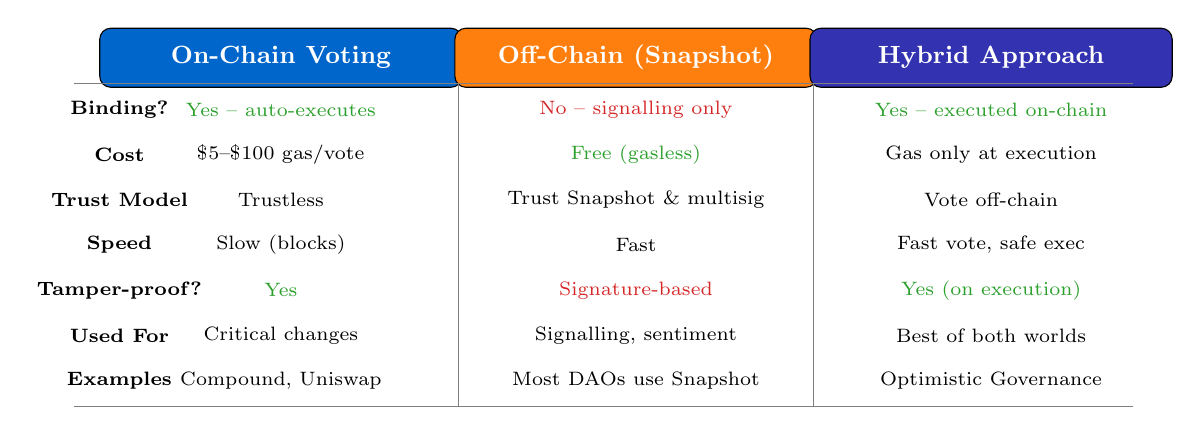
\begin{tikzpicture}[scale=0.82]
  %% On-Chain column header
  \node[draw,fill=mlblue,text=white,rounded corners=4pt,font=\small\bfseries,
        minimum width=4.6cm,minimum height=0.75cm,align=center]
        at (0,2.9) {On-Chain Voting};
  %% Off-Chain column header
  \node[draw,fill=mlorange,text=white,rounded corners=4pt,font=\small\bfseries,
        minimum width=4.6cm,minimum height=0.75cm,align=center]
        at (5.5,2.9) {Off-Chain (Snapshot)};
  %% Hybrid column header
  \node[draw,fill=mlpurple,text=white,rounded corners=4pt,font=\small\bfseries,
        minimum width=4.6cm,minimum height=0.75cm,align=center]
        at (11.0,2.9) {Hybrid Approach};

  %% Row labels
  \node[font=\scriptsize\bfseries,align=right] at (-2.5,2.1) {Binding?};
  \node[font=\scriptsize\bfseries,align=right] at (-2.5,1.4) {Cost};
  \node[font=\scriptsize\bfseries,align=right] at (-2.5,0.7) {Trust Model};
  \node[font=\scriptsize\bfseries,align=right] at (-2.5,0.0) {Speed};
  \node[font=\scriptsize\bfseries,align=right] at (-2.5,-0.7) {Tamper-proof?};
  \node[font=\scriptsize\bfseries,align=right] at (-2.5,-1.4) {Used For};
  \node[font=\scriptsize\bfseries,align=right] at (-2.5,-2.1) {Examples};

  %% On-Chain values
  \node[font=\scriptsize,text=mlgreen,align=center] at (0,2.1) {Yes -- auto-executes};
  \node[font=\scriptsize,align=center] at (0,1.4) {\$5--\$100 gas/vote};
  \node[font=\scriptsize,align=center] at (0,0.7) {Trustless};
  \node[font=\scriptsize,align=center] at (0,0.0) {Slow (blocks)};
  \node[font=\scriptsize,text=mlgreen,align=center] at (0,-0.7) {Yes};
  \node[font=\scriptsize,align=center] at (0,-1.4) {Critical changes};
  \node[font=\scriptsize,align=center] at (0,-2.1) {Compound, Uniswap};

  %% Off-Chain values
  \node[font=\scriptsize,text=mlred,align=center] at (5.5,2.1) {No -- signalling only};
  \node[font=\scriptsize,text=mlgreen,align=center] at (5.5,1.4) {Free (gasless)};
  \node[font=\scriptsize,align=center] at (5.5,0.7) {Trust Snapshot \& multisig};
  \node[font=\scriptsize,align=center] at (5.5,0.0) {Fast};
  \node[font=\scriptsize,text=mlred,align=center] at (5.5,-0.7) {Signature-based};
  \node[font=\scriptsize,align=center] at (5.5,-1.4) {Signalling, sentiment};
  \node[font=\scriptsize,align=center] at (5.5,-2.1) {Most DAOs use Snapshot};

  %% Hybrid values
  \node[font=\scriptsize,text=mlgreen,align=center] at (11.0,2.1) {Yes -- executed on-chain};
  \node[font=\scriptsize,align=center] at (11.0,1.4) {Gas only at execution};
  \node[font=\scriptsize,align=center] at (11.0,0.7) {Vote off-chain};
  \node[font=\scriptsize,align=center] at (11.0,0.0) {Fast vote, safe exec};
  \node[font=\scriptsize,text=mlgreen,align=center] at (11.0,-0.7) {Yes (on execution)};
  \node[font=\scriptsize,align=center] at (11.0,-1.4) {Best of both worlds};
  \node[font=\scriptsize,align=center] at (11.0,-2.1) {Optimistic Governance};

  %% Divider lines
  \draw[mlgray,thin] (-3.2,2.5) -- (13.2,2.5);
  \draw[mlgray,thin] (-3.2,-2.5) -- (13.2,-2.5);
  \draw[mlgray,thin] (2.75,2.5) -- (2.75,-2.5);
  \draw[mlgray,thin] (8.25,2.5) -- (8.25,-2.5);
\end{tikzpicture}
\vspace{1mm}
\begin{center}
\footnotesize\textit{Most large DAOs use off-chain Snapshot for signalling and on-chain Governor for binding execution}
\end{center}
\bottomnote{Gas cost is the primary barrier to on-chain participation -- a single governance vote on Ethereum mainnet costs \$20--\$150 in gas}
\end{frame}

% Frame 18: On-Chain Voting Power [fragile] -- CODE FRAME 2
\begin{frame}[fragile]{On-Chain Voting Power}
\begin{columns}[T]
\column{0.52\textwidth}
\begin{lstlisting}[language=Solidity,basicstyle=\ttfamily\tiny,
  caption={ERC20Votes: Voting Power Tracking}]
// ERC20Votes: Voting Power Tracking
contract VotingPower is ERC20 {
    mapping(address => address)
        public delegates;
    mapping(address => uint256[])
        internal checkpoints;

    function delegate(
        address delegatee
    ) external {
        delegates[msg.sender] =
            delegatee;
        _moveVotingPower(
            msg.sender,
            delegatee,
            balanceOf(msg.sender));
    }

    function getVotes(
        address account
    ) external view returns (uint256) {
        uint256[] storage ckpts =
            checkpoints[account];
        return ckpts.length == 0
            ? 0
            : ckpts[ckpts.length - 1];
    }
}
\end{lstlisting}

\column{0.48\textwidth}
\vspace{2mm}
\begin{block}{Delegation}
\footnotesize
\begin{itemize}
  \item Token holders assign voting power to a \textbf{delegatee} without transferring tokens
  \item Delegatee votes on behalf of all delegators
  \item Delegation can be revoked at any time
\end{itemize}
\end{block}
\vspace{2mm}
\begin{block}{Checkpoint Mechanism}
\footnotesize
\begin{itemize}
  \item Every balance change writes a new \textbf{checkpoint} (block number + amount)
  \item Enables historical lookup: ``What was Alice's voting power at block X?''
  \item Prevents flash-loan attacks by using the \textbf{snapshot block} (proposal creation block)
\end{itemize}
\end{block}
\vspace{2mm}
\begin{exampleblock}{ERC20Votes Standard}
\footnotesize
OpenZeppelin ERC20Votes implements this pattern. Used by UNI, COMP, ARB, OP governance tokens. The \texttt{getPastVotes()} function is the snapshot query.
\end{exampleblock}
\end{columns}
\bottomnote{Snapshot-at-proposal-block is the key anti-manipulation mechanism -- buying tokens after a proposal is created grants no voting power}
\end{frame}

% Frame 19: Simple Token Voting
\begin{frame}{Simple Token Voting}
\begin{columns}[T]
\column{0.48\textwidth}
\begin{block}{Mechanics}
\footnotesize
\begin{itemize}
  \item \textbf{1 token = 1 vote} -- voting power proportional to holdings
  \item \textbf{Majority wins}: For votes $>$ Against votes (simple) or $>$50\% of total (absolute)
  \item \textbf{Quorum threshold}: minimum participation required (e.g., 4\% of supply)
  \item \textbf{Participation}: typically 5--15\% of circulating supply votes
\end{itemize}
\end{block}
\vspace{2mm}
\begin{alertblock}{The Plutocracy Problem}
\footnotesize
\begin{itemize}
  \item Wealth \(\equiv\) governance power
  \item Top 10 wallets in Uniswap control \textasciitilde70\% of votes
  \item Whale can single-handedly pass proposals
  \item Retail holders face high gas costs with negligible voting impact
\end{itemize}
\end{alertblock}
\vspace{1mm}
\begin{exampleblock}{Voter Apathy}
\footnotesize
Typical DAO turnout: \textless10\% of eligible tokens. Compound governance: many proposals pass with \textless2\% participation.
\end{exampleblock}

\column{0.52\textwidth}
\vspace{2mm}
\begin{center}
\textbf{\small Vote Distribution: Proposal XYZ}
\end{center}
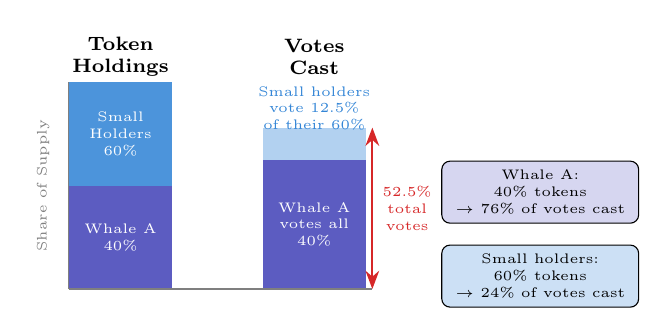
\begin{tikzpicture}[scale=0.82]
  %% Stacked bar: Token Holdings vs Actual Votes
  %% Left bar: Token Holdings
  \node[font=\scriptsize\bfseries,align=center] at (1.0,3.6) {Token\\Holdings};
  \fill[mlpurple!80] (0.2,0) rectangle (1.8,1.6);
  \fill[mlblue!70] (0.2,1.6) rectangle (1.8,3.2);
  \node[font=\tiny,text=white,align=center] at (1.0,0.8) {Whale A\\40\%};
  \node[font=\tiny,text=white,align=center] at (1.0,2.4) {Small\\Holders\\60\%};

  %% Right bar: Actual Votes Cast
  \node[font=\scriptsize\bfseries,align=center] at (4.0,3.6) {Votes\\Cast};
  \fill[mlpurple!80] (3.2,0) rectangle (4.8,2.0);
  \fill[mlblue!30] (3.2,2.0) rectangle (4.8,2.5);
  \node[font=\tiny,text=white,align=center] at (4.0,1.0) {Whale A\\votes all\\40\%};
  \node[font=\tiny,text=mlblue!80,align=center] at (4.0,2.8) {Small holders\\vote 12.5\%\\of their 60\%};

  %% Participation arrow annotation
  \draw[{Stealth}-{Stealth},thick,mlred] (4.9,0) -- (4.9,2.5)
        node[midway,right,font=\tiny,text=mlred,align=center] {52.5\%\\total\\votes};

  %% Y-axis
  \draw[thin,mlgray] (0.2,0) -- (0.2,3.2);
  \node[font=\tiny,text=mlgray,rotate=90] at (-0.2,1.6) {Share of Supply};

  %% Horizontal zero line
  \draw[thin,mlgray] (0.2,0) -- (4.9,0);

  %% Effective power labels
  \node[draw,fill=mlpurple!20,rounded corners=3pt,
        font=\tiny,align=center,minimum width=2.5cm]
        at (7.5,1.5) {Whale A:\\40\% tokens\\\(\rightarrow\) 76\% of votes cast};
  \node[draw,fill=mlblue!20,rounded corners=3pt,
        font=\tiny,align=center,minimum width=2.5cm]
        at (7.5,0.2) {Small holders:\\60\% tokens\\\(\rightarrow\) 24\% of votes cast};
\end{tikzpicture}
\end{columns}
\bottomnote{Simple token voting is simple to implement but systematically amplifies whale power relative to their token share due to voter apathy}
\end{frame}

% Frame 20: Quadratic Voting
\begin{frame}{Quadratic Voting}
\begin{columns}[T]
\column{0.48\textwidth}
\begin{block}{Formula \& Mechanics}
\footnotesize
Cost to cast $n$ votes:\vspace{1mm}
\[
\text{Cost} = n^2 \text{ credits} \quad\Longleftrightarrow\quad n = \sqrt{\text{credits}}
\]
\vspace{1mm}
\begin{center}
\footnotesize
\begin{tabular}{ccc}
\toprule
Votes ($n$) & Credits Used & Marginal Cost \\
\midrule
1 & 1 & 1 \\
2 & 4 & 3 \\
3 & 9 & 5 \\
5 & 25 & 7 \\
10 & 100 & 15 \\
\bottomrule
\end{tabular}
\end{center}
\vspace{1mm}
Each additional vote costs more -- expensive to dominate.
\end{block}
\vspace{2mm}
\begin{alertblock}{Sybil Vulnerability}
\footnotesize
Splitting tokens across many wallets cheaply obtains more quadratic votes. Requires robust identity or anti-Sybil mechanism (e.g., Gitcoin Passport, Proof of Humanity).
\end{alertblock}

\column{0.52\textwidth}
\vspace{2mm}
\begin{center}
\textbf{\small Token Voting vs Quadratic Voting}
\end{center}
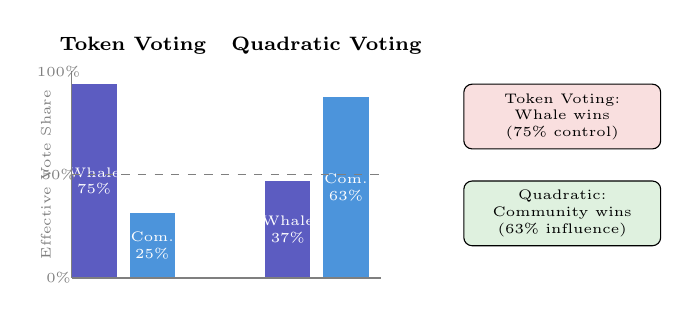
\begin{tikzpicture}[scale=0.82]
  %% Two grouped bars: Whale vs Community
  %% Bar width 0.7, gap 0.3 between groups

  %% Token Voting group (left)
  \node[font=\scriptsize\bfseries] at (1.15,3.6) {Token Voting};
  \fill[mlpurple!80] (0.2,0) rectangle (0.9,3.0);
  \fill[mlblue!70] (1.1,0) rectangle (1.8,1.0);
  \node[font=\tiny,text=white,align=center] at (0.55,1.5) {Whale\\75\%};
  \node[font=\tiny,text=white,align=center] at (1.45,0.5) {Com.\\25\%};

  %% Quadratic Voting group (right)
  \node[font=\scriptsize\bfseries] at (4.15,3.6) {Quadratic Voting};
  \fill[mlpurple!80] (3.2,0) rectangle (3.9,1.5);
  \fill[mlblue!70] (4.1,0) rectangle (4.8,2.8);
  \node[font=\tiny,text=white,align=center] at (3.55,0.75) {Whale\\37\%};
  \node[font=\tiny,text=white,align=center] at (4.45,1.4) {Com.\\63\%};

  %% Y-axis
  \draw[thin,mlgray] (0.2,0) -- (0.2,3.2);
  \node[font=\tiny,text=mlgray,rotate=90] at (-0.2,1.6) {Effective Vote Share};
  \draw[thin,mlgray] (0.2,0) -- (5.0,0);

  %% Y labels
  \node[font=\tiny,text=mlgray] at (-0.0,0) {0\%};
  \node[font=\tiny,text=mlgray] at (-0.0,1.6) {50\%};
  \node[font=\tiny,text=mlgray] at (-0.0,3.2) {100\%};
  \draw[thin,mlgray,dashed] (0.2,1.6) -- (5.0,1.6);

  %% Outcome labels
  \node[draw,fill=mlred!15,rounded corners=3pt,
        font=\tiny,align=center,minimum width=2.5cm]
        at (7.8,2.5) {Token Voting:\\Whale wins\\(75\% control)};
  \node[draw,fill=mlgreen!15,rounded corners=3pt,
        font=\tiny,align=center,minimum width=2.5cm]
        at (7.8,1.0) {Quadratic:\\Community wins\\(63\% influence)};
\end{tikzpicture}
\vspace{1mm}
\footnotesize Scenario: 1 whale (1000 tokens) vs 100 community members (10 tokens each)
\end{columns}
\bottomnote{Quadratic voting used in Gitcoin Grants (\$50M+ distributed); radical markets theory shows it achieves Pareto-efficient collective decisions}
\end{frame}

% Frame 21: Conviction Voting
\begin{frame}{Conviction Voting}
\begin{columns}[T]
\column{0.45\textwidth}
\begin{block}{Core Concept}
\footnotesize
\begin{itemize}
  \item Conviction \textbf{accumulates} the longer tokens are staked on a proposal
  \item No fixed voting deadline -- proposals pass when accumulated conviction crosses a threshold
  \item Removing stake resets conviction quickly
  \item Rewards \textbf{sustained commitment} over last-minute voting
\end{itemize}
\end{block}
\vspace{2mm}
\begin{block}{Advantages}
\footnotesize
\begin{itemize}
  \item \textbf{Attack resistance}: attacker must sustain large stake for extended period
  \item \textbf{Continuous governance}: proposals always open, no discrete voting windows
  \item \textbf{Signal clarity}: conviction reflects genuine long-term preference
  \item \textbf{Voter apathy mitigation}: passive staking counts as implicit approval
\end{itemize}
\end{block}
\vspace{2mm}
\begin{exampleblock}{Used By}
\footnotesize
1Hive (HNY token), Gitcoin (experimental), Commons Stack
\end{exampleblock}

\column{0.55\textwidth}
\vspace{2mm}
\begin{center}
\textbf{\small Conviction Accumulation Over Time}
\end{center}
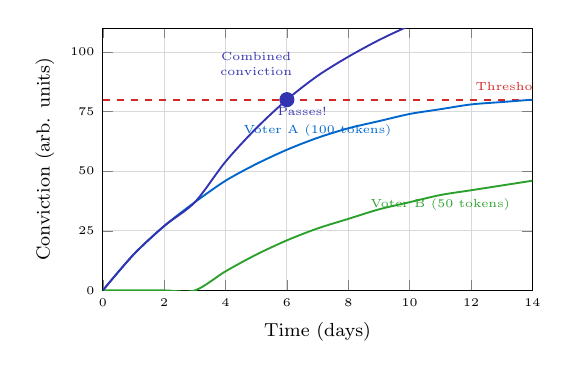
\begin{tikzpicture}[scale=0.85]
  \begin{axis}[
    width=8.0cm, height=5.5cm,
    xlabel={\footnotesize Time (days)},
    ylabel={\footnotesize Conviction (arb. units)},
    xmin=0, xmax=14,
    ymin=0, ymax=110,
    xtick={0,2,4,6,8,10,12,14},
    ytick={0,25,50,75,100},
    tick label style={font=\tiny},
    label style={font=\footnotesize},
    grid=major,
    grid style={mlgray!30},
  ]
    %% Threshold line
    \addplot[thick,mlred,dashed,domain=0:14] {80}
      node[pos=0.95,above,font=\tiny,text=mlred] {Threshold};
    %% Voter A: stakes from day 0, conviction grows fast
    \addplot[thick,mlblue,smooth] coordinates {
      (0,0)(1,15)(2,27)(3,37)(4,46)(5,53)
      (6,59)(7,64)(8,68)(9,71)(10,74)(11,76)(12,78)(13,79)(14,80)
    };
    \node[font=\tiny,text=mlblue] at (axis cs:7,67) {Voter A (100 tokens)};
    %% Voter B: joins day 3, smaller
    \addplot[thick,mlgreen,smooth] coordinates {
      (0,0)(1,0)(2,0)(3,0)(4,8)(5,15)(6,21)(7,26)
      (8,30)(9,34)(10,37)(11,40)(12,42)(13,44)(14,46)
    };
    \node[font=\tiny,text=mlgreen] at (axis cs:11,36) {Voter B (50 tokens)};
    %% Combined conviction
    \addplot[thick,mlpurple,smooth] coordinates {
      (0,0)(1,15)(2,27)(3,37)(4,54)(5,68)(6,80)(7,90)
      (8,98)(9,105)(10,111)(11,116)(12,120)(13,123)(14,126)
    };
    \node[font=\tiny,text=mlpurple,align=center] at (axis cs:5,95) {Combined\\conviction};
    %% Passes marker
    \addplot[only marks,mark=*,mark size=3pt,mlpurple]
      coordinates {(6,80)};
    \node[font=\tiny,text=mlpurple,align=center] at (axis cs:6.5,75) {Passes!};
  \end{axis}
\end{tikzpicture}
\end{columns}
\bottomnote{Conviction voting eliminates governance attacks requiring only momentary vote majority -- sustained commitment is required to pass proposals}
\end{frame}

% Frame 22: Vote Delegation
\begin{frame}{Vote Delegation}
\begin{columns}[T]
\column{0.45\textwidth}
\begin{block}{Why Delegate?}
\footnotesize
\begin{itemize}
  \item \textbf{Gas costs}: voting on-chain costs \$20--\$100; delegation is one-time
  \item \textbf{Expertise}: delegates specialize in protocol governance
  \item \textbf{Time}: retail holders lack time to analyse proposals
  \item \textbf{Participation}: delegation improves effective participation rates
\end{itemize}
\end{block}
\vspace{2mm}
\begin{block}{Liquid Democracy}
\footnotesize
\begin{itemize}
  \item Delegation can be changed or revoked at any time
  \item Transitive delegation: A delegates to B who delegates to C
  \item Override: delegator can still vote directly if they choose
  \item Delegation platforms: Tally, Agora, Karma
\end{itemize}
\end{block}
\vspace{2mm}
\begin{alertblock}{Delegation Risks}
\footnotesize
Delegates can become new whales. Inactive delegates drain participation. Misaligned delegates may vote against holders' interests.
\end{alertblock}

\column{0.55\textwidth}
\vspace{2mm}
\begin{center}
\textbf{\small Delegation Graph}
\end{center}
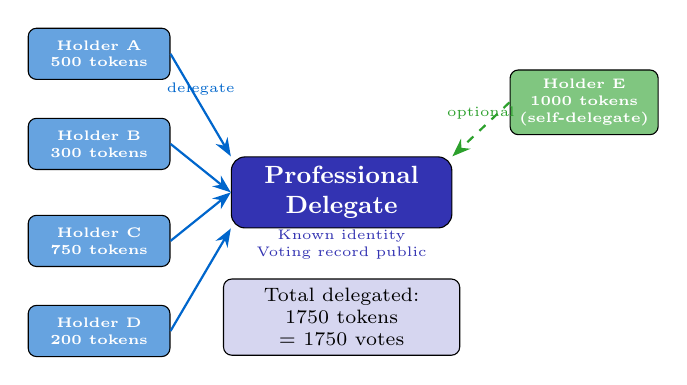
\begin{tikzpicture}[scale=0.88]
  %% Central delegate node
  \node[draw,fill=mlpurple,text=white,rounded corners=5pt,
        minimum width=2.8cm,minimum height=0.9cm,align=center,font=\small\bfseries]
        (del) at (0,0) {Professional\\Delegate};
  \node[font=\tiny,text=mlpurple,align=center] at (0,-0.75) {Known identity\\Voting record public};

  %% Small token holders delegating
  \node[draw,fill=mlblue!60,text=white,rounded corners=3pt,
        minimum width=1.8cm,minimum height=0.65cm,align=center,font=\tiny\bfseries]
        (h1) at (-3.5, 2.0) {Holder A\\500 tokens};
  \node[draw,fill=mlblue!60,text=white,rounded corners=3pt,
        minimum width=1.8cm,minimum height=0.65cm,align=center,font=\tiny\bfseries]
        (h2) at (-3.5, 0.7) {Holder B\\300 tokens};
  \node[draw,fill=mlblue!60,text=white,rounded corners=3pt,
        minimum width=1.8cm,minimum height=0.65cm,align=center,font=\tiny\bfseries]
        (h3) at (-3.5,-0.7) {Holder C\\750 tokens};
  \node[draw,fill=mlblue!60,text=white,rounded corners=3pt,
        minimum width=1.8cm,minimum height=0.65cm,align=center,font=\tiny\bfseries]
        (h4) at (-3.5,-2.0) {Holder D\\200 tokens};
  \node[draw,fill=mlgreen!60,text=white,rounded corners=3pt,
        minimum width=1.8cm,minimum height=0.65cm,align=center,font=\tiny\bfseries]
        (h5) at (3.5, 1.3) {Holder E\\1000 tokens\\(self-delegate)};

  %% Delegation arrows
  \draw[-{Stealth},thick,mlblue] (h1.east) -- (del.north west)
        node[midway,above,font=\tiny,text=mlblue] {delegate};
  \draw[-{Stealth},thick,mlblue] (h2.east) -- (del.west);
  \draw[-{Stealth},thick,mlblue] (h3.east) -- (del.west);
  \draw[-{Stealth},thick,mlblue] (h4.east) -- (del.south west);
  \draw[-{Stealth},thick,mlgreen,dashed] (h5.west) -- (del.north east)
        node[midway,above,font=\tiny,text=mlgreen] {optional};

  %% Total power label
  \node[draw,fill=mlpurple!20,rounded corners=3pt,
        font=\scriptsize,align=center,minimum width=3.0cm]
        at (0,-1.8) {Total delegated:\\1750 tokens\\= 1750 votes};
\end{tikzpicture}
\end{columns}
\bottomnote{Uniswap has \textasciitilde3000 active delegates; top 10 control majority -- delegation solves participation but can recreate plutocracy}
\end{frame}

% Frame 23: Quorum and Thresholds
\begin{frame}{Quorum and Thresholds}
\vspace{1mm}
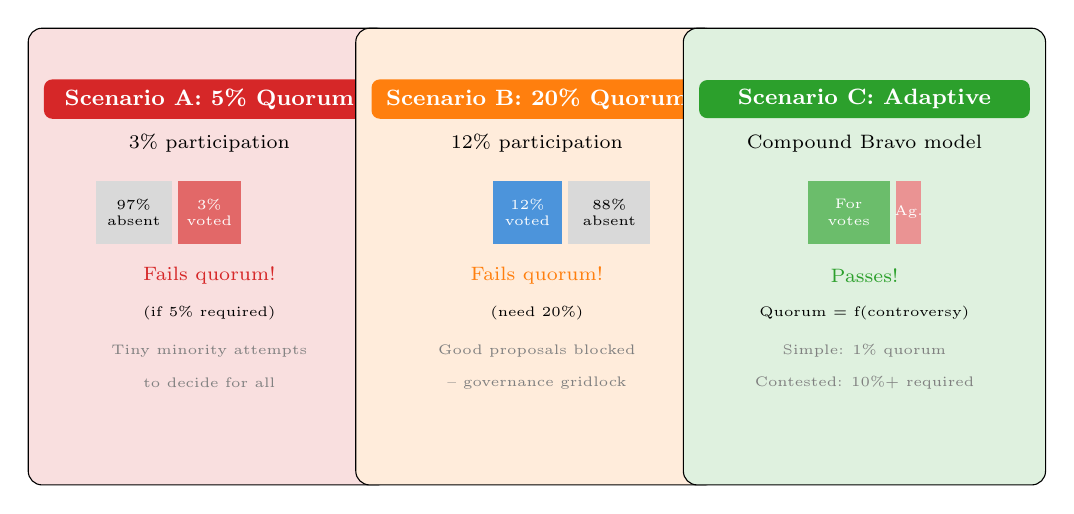
\begin{tikzpicture}[scale=0.80]
  %% Scenario A: Low quorum (5%) - vote passes with minority
  \node[draw,fill=mlred!15,rounded corners=5pt,
        minimum width=4.6cm,minimum height=5.8cm]
        at (0,0) {};
  \node[fill=mlred,text=white,rounded corners=3pt,font=\footnotesize\bfseries,
        minimum width=4.2cm,align=center]
        at (0,2.5) {Scenario A: 5\% Quorum};
  \node[font=\scriptsize,align=center,text=black] at (0,1.8) {3\% participation};
  \fill[mlred!70] (-0.5,0.2) rectangle (0.5,1.2);
  \node[font=\tiny,text=white,align=center] at (0,0.7) {3\%\\voted};
  \fill[mlgray!30] (-1.8,0.2) rectangle (-0.6,1.2);
  \node[font=\tiny,align=center] at (-1.2,0.7) {97\%\\absent};
  \node[font=\scriptsize,text=mlred,align=center] at (0,-0.3) {Fails quorum!};
  \node[font=\tiny,align=center] at (0,-0.9) {(if 5\% required)};
  \node[font=\tiny,align=center,text=mlgray] at (0,-1.5)
        {Tiny minority attempts};
  \node[font=\tiny,align=center,text=mlgray] at (0,-2.0)
        {to decide for all};

  %% Scenario B: High quorum (20%) - governance gridlock
  \node[draw,fill=mlorange!15,rounded corners=5pt,
        minimum width=4.6cm,minimum height=5.8cm]
        at (5.2,0) {};
  \node[fill=mlorange,text=white,rounded corners=3pt,font=\footnotesize\bfseries,
        minimum width=4.2cm,align=center]
        at (5.2,2.5) {Scenario B: 20\% Quorum};
  \node[font=\scriptsize,align=center,text=black] at (5.2,1.8) {12\% participation};
  \fill[mlblue!70] (4.5,0.2) rectangle (5.6,1.2);
  \node[font=\tiny,text=white,align=center] at (5.05,0.7) {12\%\\voted};
  \fill[mlgray!30] (5.7,0.2) rectangle (7.0,1.2);
  \node[font=\tiny,align=center] at (6.35,0.7) {88\%\\absent};
  \node[font=\scriptsize,text=mlorange,align=center] at (5.2,-0.3) {Fails quorum!};
  \node[font=\tiny,align=center] at (5.2,-0.9) {(need 20\%)};
  \node[font=\tiny,align=center,text=mlgray] at (5.2,-1.5)
        {Good proposals blocked};
  \node[font=\tiny,align=center,text=mlgray] at (5.2,-2.0)
        {-- governance gridlock};

  %% Scenario C: Adaptive quorum (Compound Bravo)
  \node[draw,fill=mlgreen!15,rounded corners=5pt,
        minimum width=4.6cm,minimum height=5.8cm]
        at (10.4,0) {};
  \node[fill=mlgreen,text=white,rounded corners=3pt,font=\footnotesize\bfseries,
        minimum width=4.2cm,align=center]
        at (10.4,2.5) {Scenario C: Adaptive};
  \node[font=\scriptsize,align=center,text=black] at (10.4,1.8) {Compound Bravo model};
  \fill[mlgreen!70] (9.5,0.2) rectangle (10.8,1.2);
  \node[font=\tiny,text=white,align=center] at (10.15,0.7) {For\\votes};
  \fill[mlred!50] (10.9,0.2) rectangle (11.3,1.2);
  \node[font=\tiny,text=white,align=center] at (11.1,0.7) {Ag.};
  \node[font=\scriptsize,text=mlgreen,align=center] at (10.4,-0.3) {Passes!};
  \node[font=\tiny,align=center] at (10.4,-0.9) {Quorum = f(controversy)};
  \node[font=\tiny,align=center,text=mlgray] at (10.4,-1.5)
        {Simple: 1\% quorum};
  \node[font=\tiny,align=center,text=mlgray] at (10.4,-2.0)
        {Contested: 10\%+ required};
\end{tikzpicture}
\vspace{1mm}
\begin{center}
\footnotesize
\textbf{Real thresholds:} Uniswap 4\% (\textasciitilde40M UNI) \quad Compound 1\% \quad Aave 2\% \quad Maker 3\%
\end{center}
\bottomnote{Quorum design is critical: too low enables minority capture, too high creates gridlock -- adaptive quorum is the emerging best practice}
\end{frame}

% Frame 24: Holographic Consensus
\begin{frame}{Holographic Consensus}
\begin{columns}[T]
\column{0.44\textwidth}
\begin{block}{The Scalability Problem}
\footnotesize
\begin{itemize}
  \item Every proposal needs \textbf{full quorum} -- impractical at scale
  \item Large DAOs may have hundreds of active proposals
  \item Voter fatigue: members cannot evaluate all proposals
  \item Low-quality proposals waste voter attention
\end{itemize}
\end{block}
\vspace{2mm}
\begin{block}{Holographic Solution (DAOstack)}
\footnotesize
\begin{itemize}
  \item \textbf{Prediction market} layer: GEN token stakers bet on proposal outcomes
  \item \textbf{Boosted proposals}: sufficient stake $\Rightarrow$ proposal enters boosted queue
  \item \textbf{Relaxed threshold}: boosted proposals pass with simple relative majority (no quorum)
  \item \textbf{Incentive alignment}: correct stakers earn rewards; incorrect lose stake
\end{itemize}
\end{block}
\vspace{2mm}
\begin{exampleblock}{Key Property}
\footnotesize
A small, informed minority can surface important proposals to the full DAO attention -- \textit{holographic} scaling.
\end{exampleblock}

\column{0.56\textwidth}
\vspace{2mm}
\begin{center}
\textbf{\small Holographic Consensus Flow}
\end{center}
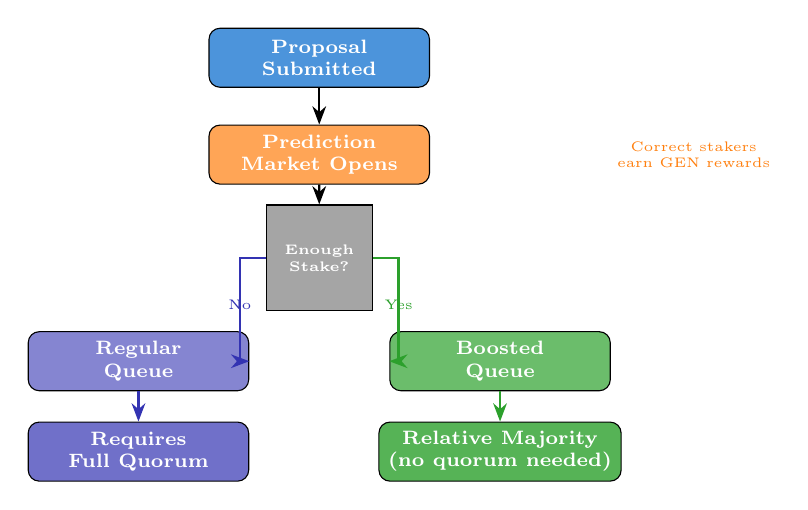
\begin{tikzpicture}[scale=0.82]
  %% Proposal submitted
  \node[draw,fill=mlblue!70,text=white,rounded corners=4pt,
        minimum width=2.8cm,minimum height=0.75cm,align=center,font=\scriptsize\bfseries]
        (prop) at (0,3.5) {Proposal\\Submitted};
  %% Prediction market
  \node[draw,fill=mlorange!70,text=white,rounded corners=4pt,
        minimum width=2.8cm,minimum height=0.75cm,align=center,font=\scriptsize\bfseries]
        (pm) at (0,2.0) {Prediction\\Market Opens};
  %% Decision: enough stake?
  \node[draw,fill=mlgray!70,text=white,regular polygon,regular polygon sides=4,
        minimum width=1.4cm,minimum height=1.4cm,align=center,font=\tiny\bfseries,
        inner sep=1pt]
        (dec) at (0,0.4) {Enough\\Stake?};
  %% Boosted path
  \node[draw,fill=mlgreen!70,text=white,rounded corners=4pt,
        minimum width=2.8cm,minimum height=0.75cm,align=center,font=\scriptsize\bfseries]
        (boost) at (2.8,-1.2) {Boosted\\Queue};
  \node[draw,fill=mlgreen!80,text=white,rounded corners=4pt,
        minimum width=2.8cm,minimum height=0.75cm,align=center,font=\scriptsize\bfseries]
        (pass) at (2.8,-2.6) {Relative Majority\\(no quorum needed)};
  %% Regular path
  \node[draw,fill=mlpurple!60,text=white,rounded corners=4pt,
        minimum width=2.8cm,minimum height=0.75cm,align=center,font=\scriptsize\bfseries]
        (reg) at (-2.8,-1.2) {Regular\\Queue};
  \node[draw,fill=mlpurple!70,text=white,rounded corners=4pt,
        minimum width=2.8cm,minimum height=0.75cm,align=center,font=\scriptsize\bfseries]
        (qpas) at (-2.8,-2.6) {Requires\\Full Quorum};

  %% Arrows
  \draw[-{Stealth},thick] (prop.south) -- (pm.north);
  \draw[-{Stealth},thick] (pm.south) -- (dec.north);
  \draw[-{Stealth},thick,mlgreen] (dec.east) -- ++(0.4,0) |- (boost.west)
        node[pos=0.3,above,font=\tiny,text=mlgreen] {Yes};
  \draw[-{Stealth},thick,mlpurple] (dec.west) -- ++(-0.4,0) |- (reg.east)
        node[pos=0.3,above,font=\tiny,text=mlpurple] {No};
  \draw[-{Stealth},thick,mlgreen] (boost.south) -- (pass.north);
  \draw[-{Stealth},thick,mlpurple] (reg.south) -- (qpas.north);

  %% Reward label
  \node[font=\tiny,text=mlorange,align=center] at (5.8,2.0)
        {Correct stakers\\earn GEN rewards};
\end{tikzpicture}
\end{columns}
\bottomnote{DAOstack's Alchemy uses holographic consensus; Genesis DAO (DAOstack's own DAO) processed 1000+ proposals using this mechanism}
\end{frame}

% Frame 25: Timelocks and Execution
\begin{frame}{Timelocks and Execution}
\vspace{2mm}
\centering
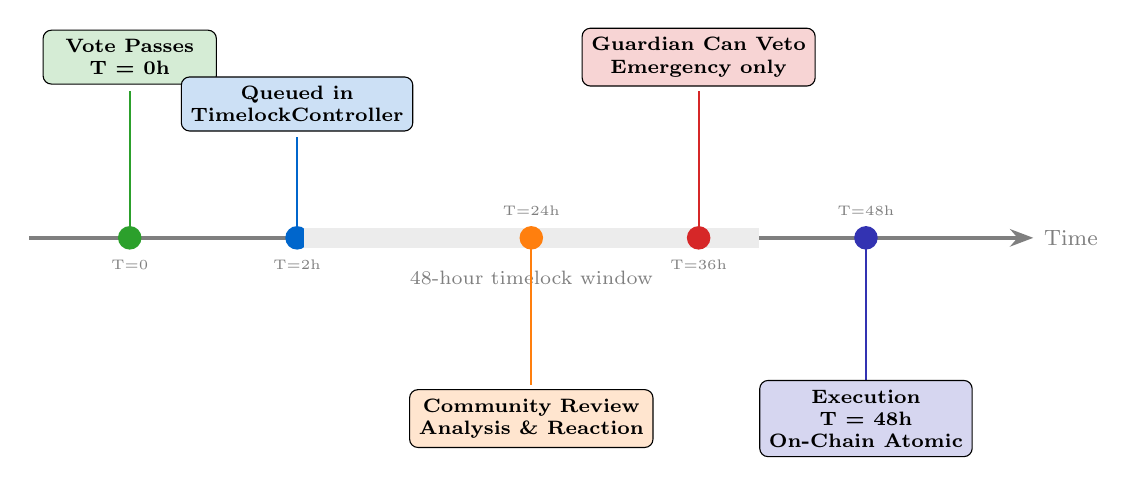
\begin{tikzpicture}[scale=0.85]
  %% Timeline axis
  \draw[-{Stealth},very thick,mlgray] (-0.5,0) -- (14.5,0)
        node[right,font=\footnotesize] {Time};

  %% Event markers on timeline
  %% T=0: Vote passes
  \fill[mlgreen] (1.0,0) circle (5pt);
  \draw[mlgreen,thick] (1.0,0) -- (1.0,2.2);
  \node[draw,fill=mlgreen!20,rounded corners=3pt,
        font=\scriptsize\bfseries,align=center,minimum width=2.2cm]
        at (1.0,2.7) {Vote Passes\\T = 0h};

  %% T=2h: Queued in timelock
  \fill[mlblue] (3.5,0) circle (5pt);
  \draw[mlblue,thick] (3.5,0) -- (3.5,1.5);
  \node[draw,fill=mlblue!20,rounded corners=3pt,
        font=\scriptsize\bfseries,align=center,minimum width=2.2cm]
        at (3.5,2.0) {Queued in\\TimelockController};

  %% Timelock zone shading
  \fill[mlgray!15] (3.6,0.15) rectangle (10.4,-0.15);
  \node[font=\scriptsize,text=mlgray,align=center] at (7.0,-0.6) {48-hour timelock window};

  %% T=24h: Community review
  \fill[mlorange] (7.0,0) circle (5pt);
  \draw[mlorange,thick] (7.0,0) -- (7.0,-2.2);
  \node[draw,fill=mlorange!20,rounded corners=3pt,
        font=\scriptsize\bfseries,align=center,minimum width=2.4cm]
        at (7.0,-2.7) {Community Review\\Analysis \& Reaction};

  %% T=36h: Guardian veto window
  \fill[mlred] (9.5,0) circle (5pt);
  \draw[mlred,thick] (9.5,0) -- (9.5,2.2);
  \node[draw,fill=mlred!20,rounded corners=3pt,
        font=\scriptsize\bfseries,align=center,minimum width=2.4cm]
        at (9.5,2.7) {Guardian Can Veto\\Emergency only};

  %% T=48h: Execution
  \fill[mlpurple] (12.0,0) circle (5pt);
  \draw[mlpurple,thick] (12.0,0) -- (12.0,-2.2);
  \node[draw,fill=mlpurple!20,rounded corners=3pt,
        font=\scriptsize\bfseries,align=center,minimum width=2.4cm]
        at (12.0,-2.7) {Execution\\T = 48h\\On-Chain Atomic};

  %% Time labels on axis
  \node[font=\tiny,text=mlgray] at (1.0,-0.4) {T=0};
  \node[font=\tiny,text=mlgray] at (3.5,-0.4) {T=2h};
  \node[font=\tiny,text=mlgray] at (7.0,0.4) {T=24h};
  \node[font=\tiny,text=mlgray] at (9.5,-0.4) {T=36h};
  \node[font=\tiny,text=mlgray] at (12.0,0.4) {T=48h};
\end{tikzpicture}
\vspace{3mm}
\begin{columns}[T]
\column{0.33\textwidth}
\begin{block}{\footnotesize Why Timelocks Matter}
\scriptsize
\begin{itemize}
  \item Time to detect and react to malicious proposals
  \item Allows users to exit protocol before harmful changes apply
  \item Emergency guardian veto as last resort (multisig)
\end{itemize}
\end{block}
\column{0.33\textwidth}
\begin{block}{\footnotesize OZ TimelockController}
\scriptsize
\begin{itemize}
  \item Standard: 24h or 48h delay
  \item Cancellation: Proposer can cancel queued tx
  \item Grace period: tx expires if not executed within 14 days
\end{itemize}
\end{block}
\column{0.33\textwidth}
\begin{alertblock}{\footnotesize Real Incidents}
\scriptsize
\begin{itemize}
  \item Beanstalk (2022): No timelock $\Rightarrow$ \$182M flash-loan governance attack in one block
  \item Compound: 2-day timelock saved treasury from a misconfigured proposal
\end{itemize}
\end{alertblock}
\end{columns}
\bottomnote{Timelocks are the single most important governance security mechanism -- Beanstalk lost \$182M due to zero timelock on governance execution}
\end{frame}

% Frame 26: Section 2 Summary
\begin{frame}{Section 2 Summary: Voting Mechanisms \& Token Governance}
\vspace{2mm}
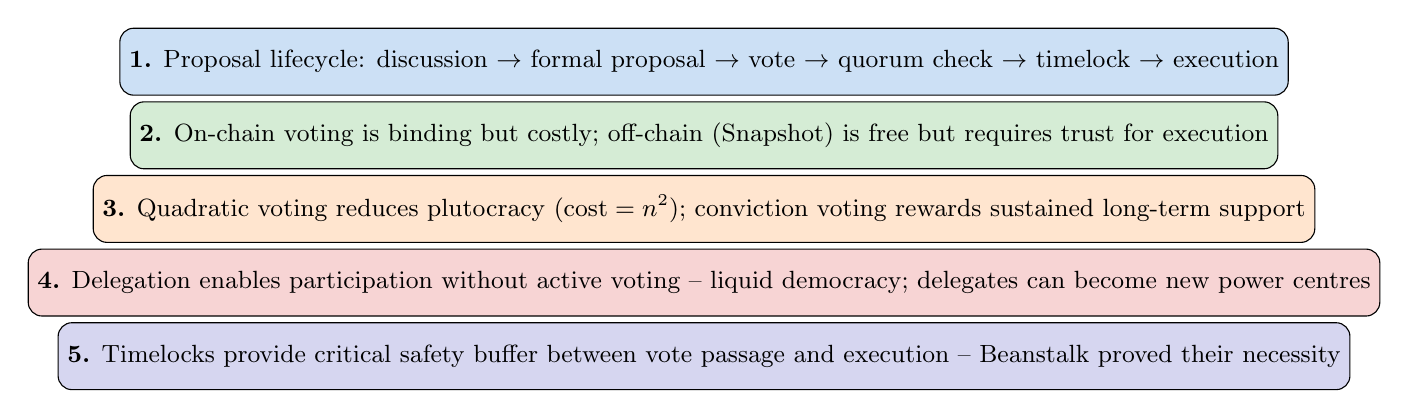
\begin{tikzpicture}[scale=0.85]
  %% Box 1
  \node[draw,fill=mlblue!20,rounded corners=5pt,
        minimum width=14.5cm,minimum height=0.85cm,align=center,font=\small]
        at (0, 2.4)
        {\textbf{1.} Proposal lifecycle: discussion \(\to\) formal proposal \(\to\) vote \(\to\) quorum check \(\to\) timelock \(\to\) execution};
  %% Box 2
  \node[draw,fill=mlgreen!20,rounded corners=5pt,
        minimum width=14.5cm,minimum height=0.85cm,align=center,font=\small]
        at (0, 1.3)
        {\textbf{2.} On-chain voting is binding but costly; off-chain (Snapshot) is free but requires trust for execution};
  %% Box 3
  \node[draw,fill=mlorange!20,rounded corners=5pt,
        minimum width=14.5cm,minimum height=0.85cm,align=center,font=\small]
        at (0, 0.2)
        {\textbf{3.} Quadratic voting reduces plutocracy (\(\text{cost}=n^2\)); conviction voting rewards sustained long-term support};
  %% Box 4
  \node[draw,fill=mlred!20,rounded corners=5pt,
        minimum width=14.5cm,minimum height=0.85cm,align=center,font=\small]
        at (0,-0.9)
        {\textbf{4.} Delegation enables participation without active voting -- liquid democracy; delegates can become new power centres};
  %% Box 5
  \node[draw,fill=mlpurple!20,rounded corners=5pt,
        minimum width=14.5cm,minimum height=0.85cm,align=center,font=\small]
        at (0,-2.0)
        {\textbf{5.} Timelocks provide critical safety buffer between vote passage and execution -- Beanstalk proved their necessity};
\end{tikzpicture}
\vspace{4mm}
\begin{center}

\begin{tikzpicture}
  \node[draw,fill=mlpurple,text=white,rounded corners=6pt,
        minimum width=10cm,minimum height=0.8cm,align=center,font=\small\bfseries]
        at (0,0) {Next: Section 3 -- Treasury Management \& Token Economics};
\end{tikzpicture}
\end{center}
\bottomnote{Section 2 complete | Key insight: voting mechanism design determines whether a DAO is democratic or plutocratic in practice}
\end{frame}

%% ============================================================
%% SECTION 3: TREASURY MANAGEMENT & ECONOMICS (Frames 27-38)
%% ============================================================
\section{Treasury Management \& Economics}

% Frame 27: Section 3 Divider
\begin{frame}{Section 3: Treasury Management \& Economics}
\vspace{4mm}
\begin{beamercolorbox}[sep=12pt,center,rounded=true,shadow=true]{palette quaternary}
{\Large\bfseries Section 3: Treasury Management \& Economics}\\[6pt]
{\normalsize How DAOs manage billions in assets and design sustainable token economies}
\end{beamercolorbox}
\vspace{2mm}
\begin{columns}[T]
\column{0.50\textwidth}
\textbf{\textcolor{mlpurple}{In this section you will learn:}}
\begin{itemize}\setlength\itemsep{5pt}
  \item Multi-sig treasury architecture (Gnosis Safe)
  \item Treasury diversification and risk management
  \item Grant programs and budget allocation
  \item Token economics: inflation, buybacks, and sustainability
\end{itemize}
\column{0.48\textwidth}
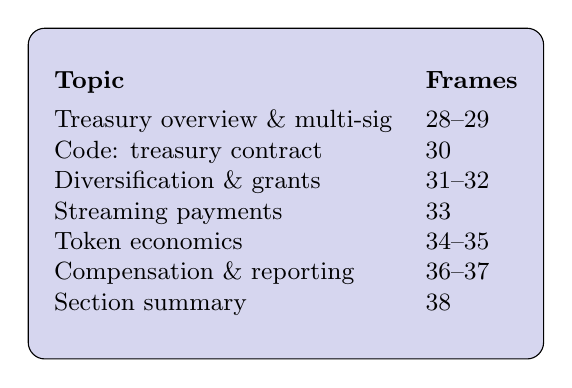
\begin{tikzpicture}
  \node[draw,fill=mllavender4,rounded corners=6pt,
        minimum width=5.8cm,minimum height=4.2cm,align=center,
        font=\small] at (0,0) {%
    \begin{tabular}{ll}
      \textbf{Topic} & \textbf{Frames}\\[3pt]
      Treasury overview \& multi-sig & 28--29\\
      Code: treasury contract & 30\\
      Diversification \& grants & 31--32\\
      Streaming payments & 33\\
      Token economics & 34--35\\
      Compensation \& reporting & 36--37\\
      Section summary & 38\\
    \end{tabular}};
\end{tikzpicture}
\end{columns}
\bottomnote{Section 3 of 5 | Treasury \& Token Economics -- the financial engine of decentralised governance}
\end{frame}

% Frame 28: DAO Treasury Overview
\begin{frame}{DAO Treasury Overview}
\begin{columns}[T]
\column{0.42\textwidth}
\vspace{2mm}
\textbf{\textcolor{mlpurple}{What is a DAO Treasury?}}\\[4pt]
A DAO treasury is a collectively owned pool of digital assets controlled exclusively by on-chain governance.
\vspace{6pt}

\begin{block}{Core Functions}
\begin{itemize}\setlength\itemsep{3pt}
  \item Fund protocol development
  \item Incentivise liquidity and contributors
  \item Cover operational expenses
  \item Build protocol-owned liquidity
\end{itemize}
\end{block}
\vspace{4pt}
\begin{alertblock}{Key Risk}
Most treasuries hold 60--90\% of their value in their \emph{own} governance token.\\
A 90\% token price drop $\Rightarrow$ 90\% treasury drop.
\end{alertblock}

\column{0.56\textwidth}
\vspace{2mm}
\textbf{\textcolor{mlpurple}{Top DAO Treasuries (approximate, 2024):}}\\[4pt]
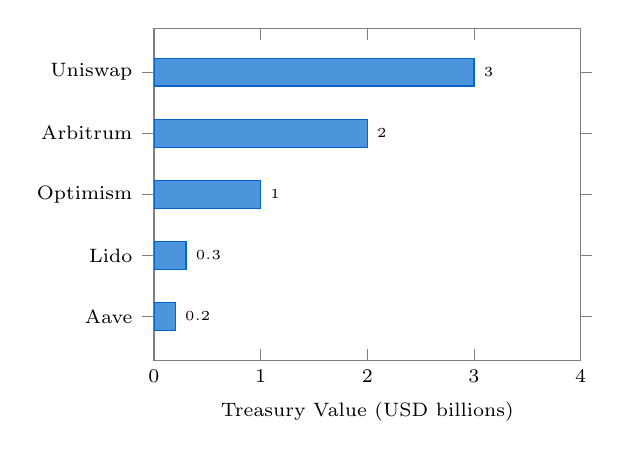
\begin{tikzpicture}
  \begin{axis}[
    xbar,
    width=7cm, height=5.8cm,
    bar width=10pt,
    xlabel={Treasury Value (USD billions)},
    xlabel style={font=\scriptsize},
    symbolic y coords={Aave,Lido,Optimism,Arbitrum,Uniswap},
    ytick=data,
    yticklabel style={font=\scriptsize},
    xticklabel style={font=\scriptsize},
    xmin=0, xmax=4,
    nodes near coords,
    nodes near coords style={font=\tiny},
    enlarge y limits=0.18,
    axis line style={draw=mlgray},
    tick style={draw=mlgray},
  ]
    \addplot[fill=mlblue!70,draw=mlblue] coordinates {
      (0.2,Aave)
      (0.3,Lido)
      (1.0,Optimism)
      (2.0,Arbitrum)
      (3.0,Uniswap)
    };
  \end{axis}
\end{tikzpicture}
\end{columns}
\bottomnote{Source: DeepDAO, Messari (2024) -- values fluctuate significantly with token prices; concentration risk is a systemic concern}
\end{frame}

% Frame 29: Multi-Sig Treasury Architecture
\begin{frame}{Multi-Sig Treasury Architecture}
\begin{columns}[T]
\column{0.58\textwidth}
\vspace{2mm}
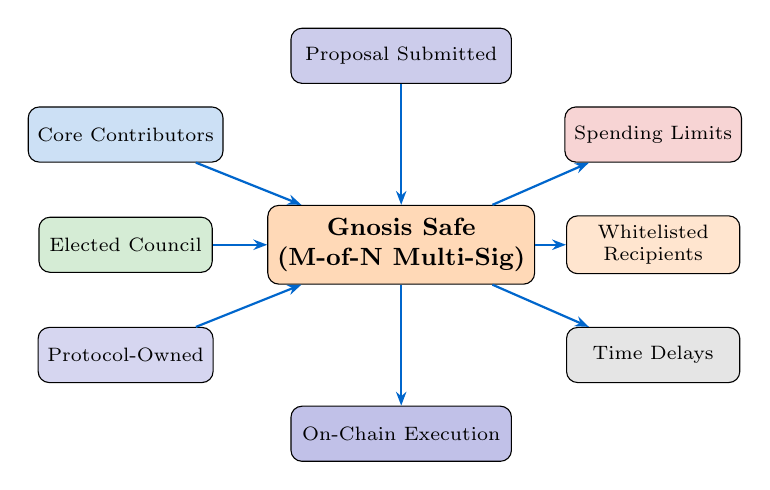
\begin{tikzpicture}[node distance=0.55cm and 1.1cm,
    every node/.style={font=\scriptsize},
    box/.style={draw,rounded corners=4pt,minimum width=2.2cm,
                minimum height=0.7cm,align=center},
    arr/.style={-{Stealth[length=5pt]},thick,mlblue}]

  %% Gnosis Safe centre
  \node[box,fill=mlorange!30,minimum width=3.2cm,minimum height=1.0cm,
        font=\small\bfseries] (safe) at (0,0) {Gnosis Safe\\(M-of-N Multi-Sig)};

  %% Signers
  \node[box,fill=mlblue!20] (cc)  at (-3.5, 1.4) {Core Contributors};
  \node[box,fill=mlgreen!20] (ec)  at (-3.5, 0.0) {Elected Council};
  \node[box,fill=mlpurple!20] (po) at (-3.5,-1.4) {Protocol-Owned};

  %% Guard modules
  \node[box,fill=mlred!20] (sp) at ( 3.2, 1.4) {Spending Limits};
  \node[box,fill=mlorange!20] (wr) at ( 3.2, 0.0) {Whitelisted\\Recipients};
  \node[box,fill=mlgray!20] (td) at ( 3.2,-1.4) {Time Delays};

  %% Proposal flow
  \node[box,fill=mllavender3,minimum width=2.8cm] (prop) at (0, 2.4) {Proposal Submitted};
  \node[box,fill=mllavender2,minimum width=2.8cm] (exec) at (0,-2.4) {On-Chain Execution};

  %% Arrows
  \draw[arr] (prop) -- (safe);
  \draw[arr] (cc)  -- (safe);
  \draw[arr] (ec)  -- (safe);
  \draw[arr] (po)  -- (safe);
  \draw[arr] (safe) -- (sp);
  \draw[arr] (safe) -- (wr);
  \draw[arr] (safe) -- (td);
  \draw[arr] (safe) -- (exec);
\end{tikzpicture}

\column{0.40\textwidth}
\vspace{2mm}
\textbf{\textcolor{mlpurple}{Common Configurations:}}
\begin{itemize}\setlength\itemsep{3pt}
  \item \textbf{3-of-5}: Small DAOs, fast decisions
  \item \textbf{5-of-9}: Large protocols, higher security
  \item \textbf{7-of-12}: Flagship treasuries
\end{itemize}
\vspace{4pt}
\begin{block}{Guard Modules}
\begin{itemize}\setlength\itemsep{2pt}
  \item Spending caps per address/period
  \item Recipient whitelists prevent draining
  \item Time delays allow community veto
\end{itemize}
\end{block}
\vspace{4pt}
\begin{block}{Transaction Flow}
\scriptsize
Proposal $\to$ Multi-sig approval $\to$ Guard checks $\to$ Execution
\end{block}
\end{columns}
\bottomnote{Gnosis Safe manages over \$50B in digital assets across the ecosystem -- the de-facto standard for DAO treasury management}
\end{frame}

% Frame 30: Treasury Management Contract
\begin{frame}[fragile]{Treasury Management Contract}
\begin{columns}[T]
\column{0.52\textwidth}
\vspace{1mm}
\begin{lstlisting}[language=Solidity,basicstyle=\ttfamily\tiny,
    caption=DAO Treasury with Spending Limits]
// DAO Treasury with Spending Limits
contract DAOTreasury {
    address public governance;
    mapping(address => uint256)
        public spendingCaps;
    uint256 public totalBudget;

    modifier onlyGovernance() {
        require(msg.sender == governance,
            "Not governance");
        _;
    }

    function allocateBudget(
        address recipient,
        uint256 amount
    ) external onlyGovernance {
        require(amount <= spendingCaps[
            recipient],
            "Exceeds spending cap");
        totalBudget -= amount;
        payable(recipient).transfer(
            amount);
        emit BudgetAllocated(
            recipient, amount);
    }
}
\end{lstlisting}

\column{0.46\textwidth}
\vspace{2mm}
\textbf{\textcolor{mlpurple}{Contract Design Explained:}}\\[6pt]

\begin{block}{Governance-Gated Execution}
\scriptsize The \texttt{onlyGovernance} modifier ensures only the governance contract (DAO) can trigger budget allocations -- no individual can spend unilaterally.
\end{block}
\vspace{3pt}
\begin{block}{Spending Caps}
\scriptsize Per-address \texttt{spendingCaps} mapping hard-limits each recipient's maximum allocation -- prevents any single grant from draining the treasury.
\end{block}
\vspace{3pt}
\begin{block}{Budget Tracking}
\scriptsize \texttt{totalBudget} is decremented atomically with each transfer -- the contract always knows its remaining balance.
\end{block}
\vspace{3pt}
\begin{block}{Event Emission}
\scriptsize \texttt{BudgetAllocated} events provide full on-chain auditability -- every expenditure is permanently recorded and searchable.
\end{block}
\end{columns}
\bottomnote{Production treasuries add: time-locks, multi-sig guards, ERC-20 support, and SafeERC20 to prevent reentrancy attacks}
\end{frame}

% Frame 31: Treasury Diversification
\begin{frame}{Treasury Diversification}
\begin{columns}[T]
\column{0.50\textwidth}
\vspace{2mm}
\textbf{\textcolor{mlpurple}{Risk-Tiered Portfolio Allocation:}}\\[4pt]
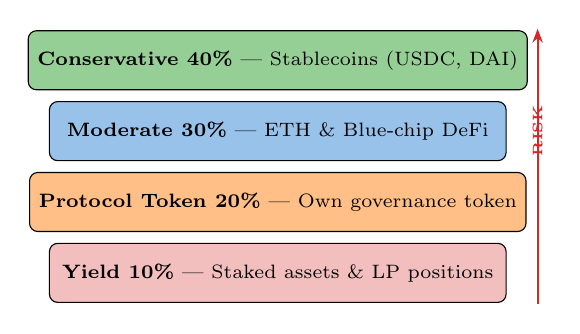
\begin{tikzpicture}[every node/.style={font=\scriptsize}]
  %% Tier bars (horizontal stacked representation)
  \node[draw,fill=mlgreen!50,minimum width=5.8cm,minimum height=0.75cm,
        align=center,rounded corners=3pt]
        at (0, 2.2) {\textbf{Conservative 40\%} --- Stablecoins (USDC, DAI)};
  \node[draw,fill=mlblue!40,minimum width=5.8cm,minimum height=0.75cm,
        align=center,rounded corners=3pt]
        at (0, 1.3) {\textbf{Moderate 30\%} --- ETH \& Blue-chip DeFi};
  \node[draw,fill=mlorange!50,minimum width=5.8cm,minimum height=0.75cm,
        align=center,rounded corners=3pt]
        at (0, 0.4) {\textbf{Protocol Token 20\%} --- Own governance token};
  \node[draw,fill=mlred!30,minimum width=5.8cm,minimum height=0.75cm,
        align=center,rounded corners=3pt]
        at (0,-0.5) {\textbf{Yield 10\%} --- Staked assets \& LP positions};

  %% Risk label
  \draw[-{Stealth[length=5pt]},thick,mlred] (3.3,-0.9) -- (3.3, 2.6)
        node[right,midway,rotate=90,font=\tiny\bfseries,text=mlred]
        {RISK};
\end{tikzpicture}
\vspace{4pt}
\begin{alertblock}{Concentration Risk}
\scriptsize If the protocol token drops 90\%, a 60\%-concentrated treasury loses \$540M on a \$1B treasury. Diversification is existential.
\end{alertblock}

\column{0.48\textwidth}
\vspace{2mm}
\textbf{\textcolor{mlpurple}{Why Each Tier?}}\\[4pt]
\begin{itemize}\setlength\itemsep{4pt}
  \item \textbf{Stablecoins}: 12--18 months of runway regardless of market conditions; pay contributors and service providers
  \item \textbf{ETH / Blue-chip}: Store of value with growth potential; widely accepted collateral
  \item \textbf{Protocol token}: Retain alignment; required for incentive programs
  \item \textbf{Yield positions}: Generate passive income to extend runway without selling
\end{itemize}
\vspace{4pt}
\begin{block}{Rebalancing Triggers}
\scriptsize Quarterly review, or immediately if any tier moves $\pm 15$pp from target.
\end{block}
\end{columns}
\bottomnote{MakerDAO's ``Endgame'' plan shifted \$500M+ from MKR to stablecoins and real-world assets to reduce concentration risk}
\end{frame}

% Frame 32: Grant Programs
\begin{frame}{Grant Programs}
\begin{columns}[T]
\column{0.48\textwidth}
\vspace{2mm}
\textbf{\textcolor{mlpurple}{Funnel: Applications to Impact}}\\[4pt]
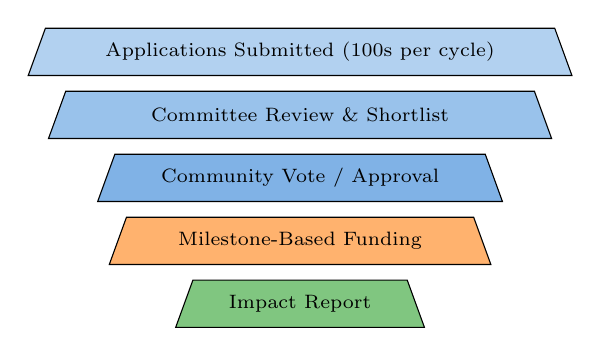
\begin{tikzpicture}[every node/.style={font=\scriptsize},
    trap/.style={draw,trapezium,trapezium left angle=70,
                 trapezium right angle=70,align=center,
                 minimum height=0.6cm}]
  \node[trap,fill=mlblue!30,minimum width=5.4cm]
        at (0, 3.6) {Applications Submitted (100s per cycle)};
  \node[trap,fill=mlblue!40,minimum width=4.4cm]
        at (0, 2.8) {Committee Review \& Shortlist};
  \node[trap,fill=mlblue!50,minimum width=3.4cm]
        at (0, 2.0) {Community Vote / Approval};
  \node[trap,fill=mlorange!60,minimum width=2.6cm]
        at (0, 1.2) {Milestone-Based Funding};
  \node[trap,fill=mlgreen!60,minimum width=1.8cm]
        at (0, 0.4) {Impact Report};
\end{tikzpicture}

\column{0.50\textwidth}
\vspace{2mm}
\textbf{\textcolor{mlpurple}{Real-World Examples:}}\\[4pt]
\begin{itemize}\setlength\itemsep{4pt}
  \item \textbf{Uniswap Grants}: \$75M allocated; development, research, and community building
  \item \textbf{Aave Grants}: Quarterly cohorts; focus on integrations and tooling
  \item \textbf{Optimism RetroPGF}: Retroactive rewards for \emph{past} public goods contributions
\end{itemize}
\vspace{4pt}
\begin{block}{Grant Categories}
\begin{tabular}{ll}
  \textbf{Development} & Protocol features, integrations\\
  \textbf{Research}    & Security, economics, governance\\
  \textbf{Community}   & Education, events, translation\\
  \textbf{Marketing}   & Awareness, partnerships\\
\end{tabular}
\end{block}
\end{columns}
\bottomnote{Milestone-based disbursement reduces risk of grant misuse -- funds released only upon verified delivery of agreed outputs}
\end{frame}

% Frame 33: Streaming Payments
\begin{frame}{Streaming Payments}
\begin{columns}[T]
\column{0.56\textwidth}
\vspace{2mm}
\textbf{\textcolor{mlpurple}{Traditional vs.\ Streaming Payment:}}\\[4pt]
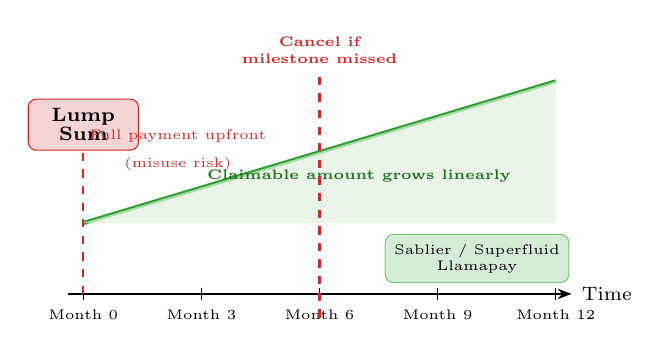
\begin{tikzpicture}[every node/.style={font=\scriptsize}]
  %% Timeline axis
  \draw[-{Stealth[length=5pt]},thick] (-0.2,0) -- (6.2,0)
        node[right] {Time};
  \foreach \x/\lbl in {0/Month 0, 1.5/Month 3, 3/Month 6,
                        4.5/Month 9, 6/Month 12}{
    \draw (\x,0.08) -- (\x,-0.08) node[below,font=\tiny] {\lbl};
  }

  %% Traditional: single lump sum at t=0
  \draw[thick,mlred,dashed] (0,0) -- (0,1.8);
  \node[fill=mlred!20,draw=mlred,rounded corners=3pt,
        minimum width=1.4cm,minimum height=0.55cm,align=center]
        at (0,2.15) {\textbf{Lump}\\[-1pt]\textbf{Sum}};
  \node[text=mlred,font=\tiny] at (1.2,2.0) {Full payment upfront};
  \node[text=mlred,font=\tiny] at (1.2,1.65) {(misuse risk)};

  %% Streaming: diagonal ramp
  \draw[thick,mlgreen,line width=1.5pt] (0,0.9) -- (6,0.9+1.8);
  \fill[mlgreen!15,opacity=0.7]
        (0,0.9) -- (6,0.9+1.8) -- (6,0.9) -- cycle;
  \node[text=mlgreen!70!black,font=\tiny\bfseries] at (3.5,1.5)
        {Claimable amount grows linearly};

  %% Protocol labels
  \node[fill=mlgreen!20,draw=mlgreen!60,rounded corners=3pt,
        minimum width=1.8cm,minimum height=0.45cm,align=center,
        font=\tiny] at (5.0,0.45) {Sablier / Superfluid\\Llamapay};

  %% Cancel marker
  \draw[mlred,thick,dashed] (3,-0.3) -- (3,2.8)
        node[above,text=mlred,font=\tiny\bfseries,align=center] {Cancel if\\milestone missed};
\end{tikzpicture}

\column{0.42\textwidth}
\vspace{2mm}
\textbf{\textcolor{mlpurple}{Why Streaming?}}\\[4pt]
\begin{itemize}\setlength\itemsep{4pt}
  \item \textbf{Reduced trust}: Recipient earns per second of work delivered
  \item \textbf{Automatic payroll}: No monthly proposal needed; contributors claim anytime
  \item \textbf{Revocable}: DAO can cancel the stream if deliverables are not met
  \item \textbf{Composable}: Streams can be used as collateral in DeFi
\end{itemize}
\vspace{4pt}
\begin{block}{Leading Protocols}
\begin{itemize}\setlength\itemsep{2pt}
  \item \textbf{Sablier}: Fixed-term streams
  \item \textbf{Superfluid}: Real-time streams with DeFi composability
  \item \textbf{Llamapay}: Simple, gas-efficient payroll
\end{itemize}
\end{block}
\end{columns}
\bottomnote{Streaming replaces the ``pay and pray'' model -- every second of non-delivery means zero incremental cost to the DAO treasury}
\end{frame}

% Frame 34: Token Economics -- Supply Side
\begin{frame}{Token Economics: Supply Side}
\begin{columns}[T]
\column{0.50\textwidth}
\vspace{2mm}
\textbf{\textcolor{mlpurple}{Supply Dynamics:}}\\[4pt]
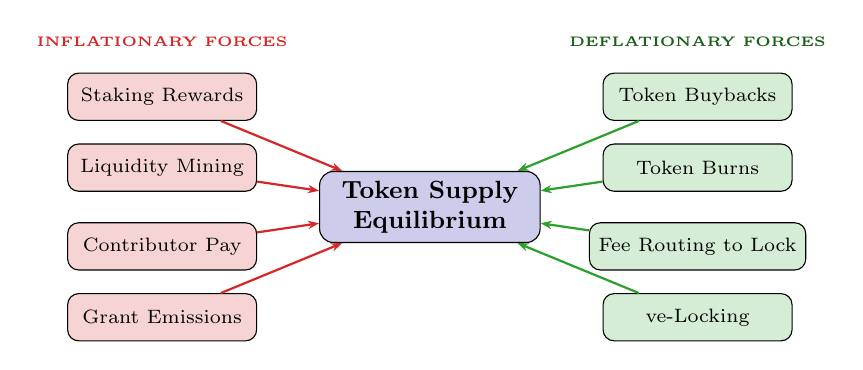
\begin{tikzpicture}[every node/.style={font=\scriptsize},
    arr/.style={-{Stealth[length=4pt]},thick}]
  %% Central balance node
  \node[draw,fill=mllavender3,rounded corners=5pt,
        minimum width=2.8cm,minimum height=0.8cm,align=center,
        font=\small\bfseries] (eq) at (0,0) {Token Supply\\Equilibrium};

  %% Inflationary forces (left)
  \node[draw,fill=mlred!20,rounded corners=4pt,
        minimum width=2.4cm,minimum height=0.6cm,align=center]
        (sr) at (-3.4, 1.4) {Staking Rewards};
  \node[draw,fill=mlred!20,rounded corners=4pt,
        minimum width=2.4cm,minimum height=0.6cm,align=center]
        (lm) at (-3.4, 0.5) {Liquidity Mining};
  \node[draw,fill=mlred!20,rounded corners=4pt,
        minimum width=2.4cm,minimum height=0.6cm,align=center]
        (cc) at (-3.4,-0.5) {Contributor Pay};
  \node[draw,fill=mlred!20,rounded corners=4pt,
        minimum width=2.4cm,minimum height=0.6cm,align=center]
        (gr) at (-3.4,-1.4) {Grant Emissions};
  \node[text=mlred,font=\tiny\bfseries] at (-3.4, 2.1)
        {INFLATIONARY FORCES};

  %% Deflationary forces (right)
  \node[draw,fill=mlgreen!20,rounded corners=4pt,
        minimum width=2.4cm,minimum height=0.6cm,align=center]
        (bu) at (3.4, 1.4) {Token Buybacks};
  \node[draw,fill=mlgreen!20,rounded corners=4pt,
        minimum width=2.4cm,minimum height=0.6cm,align=center]
        (tb) at (3.4, 0.5) {Token Burns};
  \node[draw,fill=mlgreen!20,rounded corners=4pt,
        minimum width=2.4cm,minimum height=0.6cm,align=center]
        (fr) at (3.4,-0.5) {Fee Routing to Lock};
  \node[draw,fill=mlgreen!20,rounded corners=4pt,
        minimum width=2.4cm,minimum height=0.6cm,align=center]
        (lk) at (3.4,-1.4) {ve-Locking};
  \node[text=mlgreen!60!black,font=\tiny\bfseries] at (3.4, 2.1)
        {DEFLATIONARY FORCES};

  \draw[arr,mlred]   (sr) -- (eq);
  \draw[arr,mlred]   (lm) -- (eq);
  \draw[arr,mlred]   (cc) -- (eq);
  \draw[arr,mlred]   (gr) -- (eq);
  \draw[arr,mlgreen] (bu) -- (eq);
  \draw[arr,mlgreen] (tb) -- (eq);
  \draw[arr,mlgreen] (fr) -- (eq);
  \draw[arr,mlgreen] (lk) -- (eq);
\end{tikzpicture}

\column{0.48\textwidth}
\vspace{2mm}
\textbf{\textcolor{mlpurple}{Emission Schedules Over Time:}}\\[3pt]
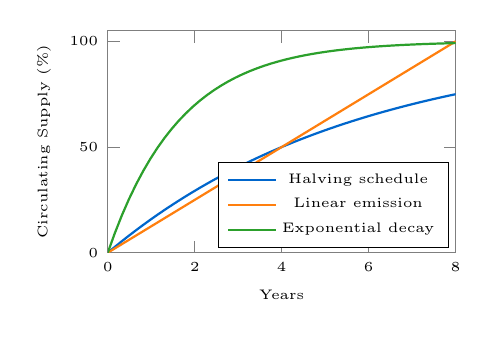
\begin{tikzpicture}
  \begin{axis}[
    width=6cm, height=4.4cm,
    xlabel={Years},
    ylabel={Circulating Supply (\%)},
    xlabel style={font=\tiny},
    ylabel style={font=\tiny},
    xticklabel style={font=\tiny},
    yticklabel style={font=\tiny},
    xmin=0, xmax=8,
    ymin=0, ymax=105,
    legend style={font=\tiny,at={(0.98,0.02)},anchor=south east},
    axis line style={draw=mlgray},
    tick style={draw=mlgray},
  ]
    %% Fixed supply (Bitcoin-like)
    \addplot[thick,mlblue,domain=0:8,samples=50]
      {100*(1 - 0.5^(x/4))};
    \addlegendentry{Halving schedule}
    %% Linear emission
    \addplot[thick,mlorange,domain=0:8,samples=2]
      {min(12.5*x, 100)};
    \addlegendentry{Linear emission}
    %% Exponential decay
    \addplot[thick,mlgreen,domain=0:8,samples=50]
      {100*(1 - exp(-0.6*x))};
    \addlegendentry{Exponential decay}
  \end{axis}
\end{tikzpicture}
\vspace{2pt}
\begin{itemize}\setlength\itemsep{2pt}
  \item \textbf{MKR}: Burned from stability fees (deflationary)
  \item \textbf{UNI}: 2\% perpetual inflation after year 4
  \item \textbf{CRV}: Decaying emission schedule over 6 years
\end{itemize}
\end{columns}
\bottomnote{Sustainable tokenomics require inflationary emissions to be offset by real protocol revenue -- ``print and hope'' fails long-term}
\end{frame}

% Frame 35: Token Economics -- Demand Side
\begin{frame}{Token Economics: Demand Side}
\begin{columns}[T]
\column{0.54\textwidth}
\vspace{2mm}
\textbf{\textcolor{mlpurple}{Value Accrual Flowchart:}}\\[4pt]
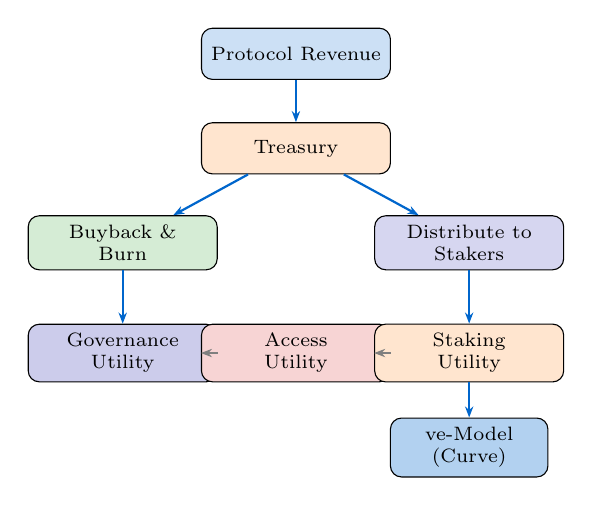
\begin{tikzpicture}[every node/.style={font=\scriptsize},
    box/.style={draw,rounded corners=4pt,minimum width=2.4cm,
                minimum height=0.65cm,align=center},
    arr/.style={-{Stealth[length=4pt]},thick,mlblue}]

  \node[box,fill=mlblue!20]    (rev)  at (0, 3.0) {Protocol Revenue};
  \node[box,fill=mlorange!20]  (trs)  at (0, 1.8) {Treasury};

  \node[box,fill=mlgreen!20]   (bbk)  at (-2.2, 0.6) {Buyback \&\\Burn};
  \node[box,fill=mlpurple!20]  (dst)  at ( 2.2, 0.6) {Distribute to\\Stakers};

  \node[box,fill=mllavender3]  (gov)  at (-2.2,-0.8) {Governance\\Utility};
  \node[box,fill=mlred!20]     (acc)  at ( 0.0,-0.8) {Access\\Utility};
  \node[box,fill=mlorange!20]  (stk)  at ( 2.2,-0.8) {Staking\\Utility};

  \node[box,fill=mlblue!30,minimum width=2.0cm] (vemod) at (2.2,-2.0)
        {ve-Model\\(Curve)};

  \draw[arr] (rev) -- (trs);
  \draw[arr] (trs) -- (bbk);
  \draw[arr] (trs) -- (dst);
  \draw[arr] (bbk) -- (gov);
  \draw[arr] (dst) -- (stk);
  \draw[arr] (stk) -- (vemod);
  \draw[arr,mlgray] (gov) -- (acc);
  \draw[arr,mlgray] (acc) -- (stk);
\end{tikzpicture}

\column{0.44\textwidth}
\vspace{2mm}
\textbf{\textcolor{mlpurple}{Utility Dimensions:}}\\[4pt]
\begin{itemize}\setlength\itemsep{4pt}
  \item \textbf{Governance}: Voting rights, proposal power, veto capability
  \item \textbf{Access}: Fee discounts, premium features, whitelist access
  \item \textbf{Staking}: Security bonds, yield, ve-locking multiplier
\end{itemize}
\vspace{4pt}
\begin{block}{The ve-Model (Curve Finance)}
\scriptsize Lock tokens for 1--4 years to receive \textbf{veCRV}:\\
\begin{itemize}\setlength\itemsep{2pt}
  \item More voting power for gauge weights
  \item Boosted liquidity rewards (up to 2.5$\times$)
  \item Share of protocol fees (3CRV)
\end{itemize}
Creates \textbf{long-term alignment}: only committed holders influence the protocol.
\end{block}
\end{columns}
\bottomnote{Token value ultimately depends on the protocol's ability to generate sustainable revenue and direct it to token holders}
\end{frame}

% Frame 36: Compensation Models
\begin{frame}{Compensation Models}
\vspace{2mm}
\textbf{\textcolor{mlpurple}{Four Approaches to DAO Contributor Compensation:}}\\[4pt]
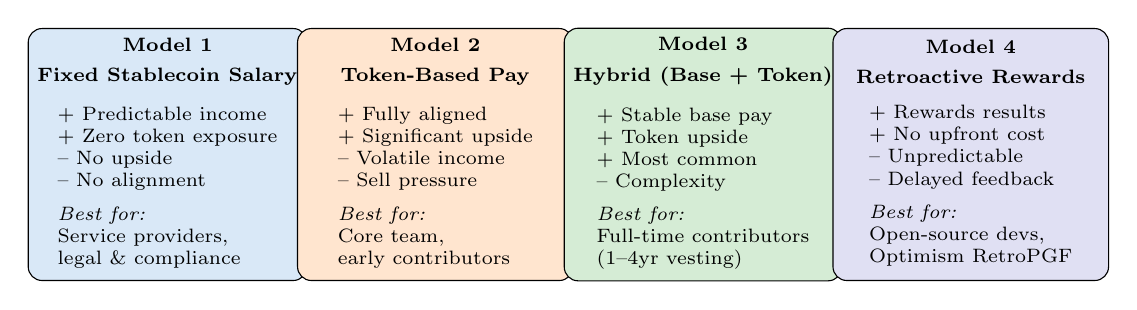
\begin{tikzpicture}[every node/.style={font=\scriptsize}]
  %% Model 1
  \node[draw,fill=mlblue!15,rounded corners=5pt,
        minimum width=3.5cm,minimum height=3.2cm,align=center]
        at (-5.1,0) {%
    \textbf{Model 1}\\[3pt]
    \textbf{Fixed Stablecoin Salary}\\[6pt]
    \begin{tabular}{l}
    + Predictable income\\
    + Zero token exposure\\
    -- No upside\\
    -- No alignment\\[4pt]
    \textit{Best for:}\\
    Service providers,\\
    legal \& compliance
    \end{tabular}};
  %% Model 2
  \node[draw,fill=mlorange!20,rounded corners=5pt,
        minimum width=3.5cm,minimum height=3.2cm,align=center]
        at (-1.7,0) {%
    \textbf{Model 2}\\[3pt]
    \textbf{Token-Based Pay}\\[6pt]
    \begin{tabular}{l}
    + Fully aligned\\
    + Significant upside\\
    -- Volatile income\\
    -- Sell pressure\\[4pt]
    \textit{Best for:}\\
    Core team,\\
    early contributors
    \end{tabular}};
  %% Model 3
  \node[draw,fill=mlgreen!20,rounded corners=5pt,
        minimum width=3.5cm,minimum height=3.2cm,align=center]
        at (1.7,0) {%
    \textbf{Model 3}\\[3pt]
    \textbf{Hybrid (Base + Token)}\\[6pt]
    \begin{tabular}{l}
    + Stable base pay\\
    + Token upside\\
    + Most common\\
    -- Complexity\\[4pt]
    \textit{Best for:}\\
    Full-time contributors\\
    (1--4yr vesting)
    \end{tabular}};
  %% Model 4
  \node[draw,fill=mlpurple!15,rounded corners=5pt,
        minimum width=3.5cm,minimum height=3.2cm,align=center]
        at (5.1,0) {%
    \textbf{Model 4}\\[3pt]
    \textbf{Retroactive Rewards}\\[6pt]
    \begin{tabular}{l}
    + Rewards results\\
    + No upfront cost\\
    -- Unpredictable\\
    -- Delayed feedback\\[4pt]
    \textit{Best for:}\\
    Open-source devs,\\
    Optimism RetroPGF
    \end{tabular}};
\end{tikzpicture}
\bottomnote{Most mature DAOs use Model 3 with 4-year vesting and 1-year cliff -- mirroring traditional startup equity compensation structures}
\end{frame}

% Frame 37: Financial Reporting & Transparency
\begin{frame}{Financial Reporting \& Transparency}
\begin{columns}[T]
\column{0.58\textwidth}
\vspace{2mm}
\textbf{\textcolor{mlpurple}{On-Chain Dashboard Mockup:}}\\[3pt]
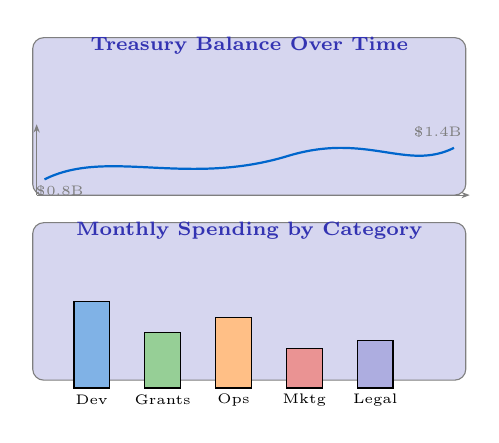
\begin{tikzpicture}[every node/.style={font=\tiny},
    panel/.style={draw=mlgray,rounded corners=4pt,fill=mllavender4}]

  %% Panel 1: Treasury balance (line chart sketch)
  \node[panel,minimum width=5.5cm,minimum height=2.0cm] at (0, 2.4) {};
  \node[font=\scriptsize\bfseries,text=mlpurple] at (0,3.3) {Treasury Balance Over Time};
  \draw[mlblue,thick] (-2.6,1.6) .. controls (-1.8,2.0) and (-0.8,1.5)
        .. (0.5,1.9) .. controls (1.5,2.2) and (2.0,1.7) .. (2.6,2.0);
  \node[text=mlgray] at (-2.4,1.45) {\$0.8B};
  \node[text=mlgray] at ( 2.4,2.2)  {\$1.4B};
  \draw[-{Stealth[length=3pt]},mlgray] (-2.7,1.4) -- (-2.7,2.3);
  \draw[-{Stealth[length=3pt]},mlgray] (-2.7,1.4) -- (2.8,1.4);

  %% Panel 2: Monthly spending (bar chart sketch)
  \node[panel,minimum width=5.5cm,minimum height=2.0cm] at (0, 0.05) {};
  \node[font=\scriptsize\bfseries,text=mlpurple] at (0,0.95) {Monthly Spending by Category};
  \node[draw,fill=mlblue!50,   minimum width=0.45cm,minimum height=1.1cm] at (-2.0,-0.5) {};
  \node[draw,fill=mlgreen!50,  minimum width=0.45cm,minimum height=0.7cm] at (-1.1,-0.7) {};
  \node[draw,fill=mlorange!50, minimum width=0.45cm,minimum height=0.9cm] at (-0.2,-0.6) {};
  \node[draw,fill=mlred!50,    minimum width=0.45cm,minimum height=0.5cm] at ( 0.7,-0.8) {};
  \node[draw,fill=mlpurple!40, minimum width=0.45cm,minimum height=0.6cm] at ( 1.6,-0.75) {};
  \node at (-2.0,-1.2) {Dev};
  \node at (-1.1,-1.2) {Grants};
  \node at (-0.2,-1.2) {Ops};
  \node at ( 0.7,-1.2) {Mktg};
  \node at ( 1.6,-1.2) {Legal};
\end{tikzpicture}

\column{0.40\textwidth}
\vspace{2mm}
\textbf{\textcolor{mlpurple}{The Transparency Advantage:}}\\[4pt]
\begin{itemize}\setlength\itemsep{4pt}
  \item Every transaction is on-chain and publicly auditable -- no hidden spending
  \item Real-time balance visible to all token holders globally
  \item Automated reporting via Dune Analytics dashboards
\end{itemize}
\vspace{4pt}
\begin{block}{Reporting Tools}
\begin{itemize}\setlength\itemsep{2pt}
  \item \textbf{DeBank}: Portfolio tracking across chains
  \item \textbf{Zerion}: Multi-wallet treasury view
  \item \textbf{Dune Analytics}: Custom SQL dashboards
  \item \textbf{Karma}: Contributor accountability
\end{itemize}
\end{block}
\vspace{4pt}
\begin{block}{Best Practice}
\scriptsize Monthly treasurer reports with on-chain proof; quarterly audits by independent firms.
\end{block}
\end{columns}
\bottomnote{Uniswap, Aave, and Compound all publish monthly treasury reports -- setting the standard for DAO financial transparency}
\end{frame}

% Frame 38: Section 3 Summary
\begin{frame}{Section 3 Summary: Treasury Management \& Economics}
\vspace{3mm}
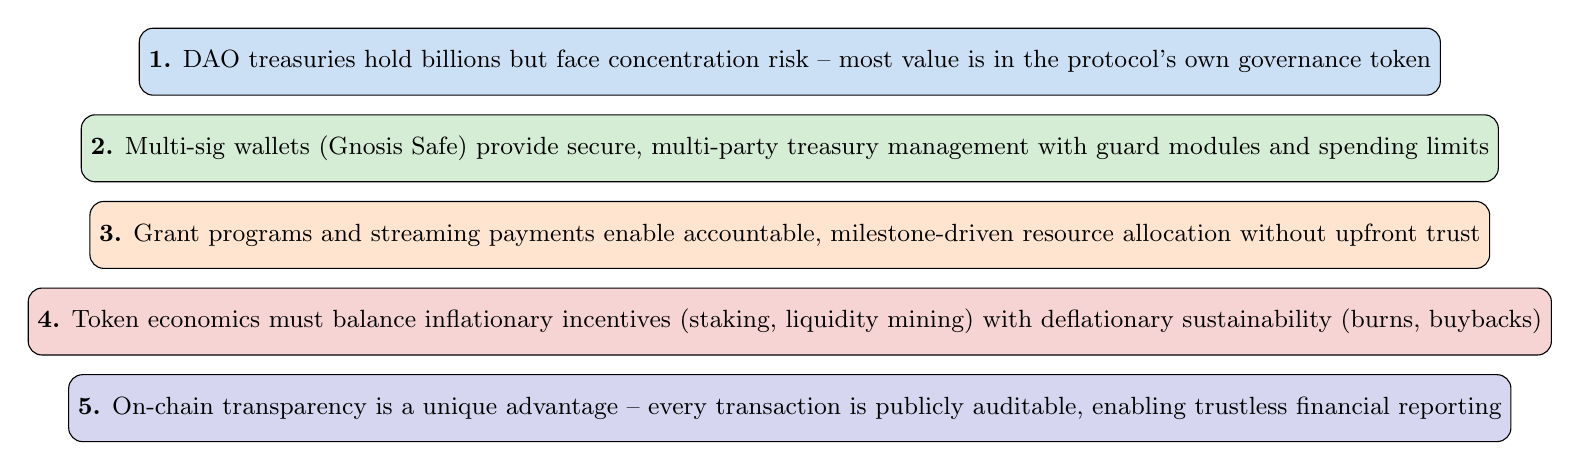
\begin{tikzpicture}[every node/.style={font=\small}]
  %% Box 1
  \node[draw,fill=mlblue!20,rounded corners=5pt,
        minimum width=14.5cm,minimum height=0.85cm,align=center,font=\small]
        at (0, 2.4)
        {\textbf{1.} DAO treasuries hold billions but face concentration risk -- most value is in the protocol's own governance token};
  %% Box 2
  \node[draw,fill=mlgreen!20,rounded corners=5pt,
        minimum width=14.5cm,minimum height=0.85cm,align=center,font=\small]
        at (0, 1.3)
        {\textbf{2.} Multi-sig wallets (Gnosis Safe) provide secure, multi-party treasury management with guard modules and spending limits};
  %% Box 3
  \node[draw,fill=mlorange!20,rounded corners=5pt,
        minimum width=14.5cm,minimum height=0.85cm,align=center,font=\small]
        at (0, 0.2)
        {\textbf{3.} Grant programs and streaming payments enable accountable, milestone-driven resource allocation without upfront trust};
  %% Box 4
  \node[draw,fill=mlred!20,rounded corners=5pt,
        minimum width=14.5cm,minimum height=0.85cm,align=center,font=\small]
        at (0,-0.9)
        {\textbf{4.} Token economics must balance inflationary incentives (staking, liquidity mining) with deflationary sustainability (burns, buybacks)};
  %% Box 5
  \node[draw,fill=mlpurple!20,rounded corners=5pt,
        minimum width=14.5cm,minimum height=0.85cm,align=center,font=\small]
        at (0,-2.0)
        {\textbf{5.} On-chain transparency is a unique advantage -- every transaction is publicly auditable, enabling trustless financial reporting};
\end{tikzpicture}
\vspace{4mm}
\begin{center}
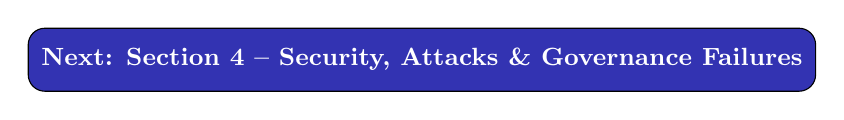
\begin{tikzpicture}
  \node[draw,fill=mlpurple,text=white,rounded corners=6pt,
        minimum width=10cm,minimum height=0.8cm,align=center,font=\small\bfseries]
        at (0,0) {Next: Section 4 -- Security, Attacks \& Governance Failures};
\end{tikzpicture}
\end{center}
\bottomnote{Section 3 complete | Key insight: treasury diversification and on-chain transparency are the foundations of long-term DAO sustainability}
\end{frame}

%% ============================================================
%% SECTION 4: Governance Attacks & Security
%% ============================================================
\section{Governance Security}

% Frame 39: Section 4 Divider
\begin{frame}
\begin{center}
\begin{beamercolorbox}[sep=12pt,center,rounded=true,shadow=true]{palette quaternary}
{\Large\bfseries Section 4: Governance Attacks \& Security}\\[6pt]
{\normalsize Understanding and defending against threats to decentralized governance}
\end{beamercolorbox}

\vspace{4mm}
\begin{columns}[t]
\column{0.5\textwidth}
\begin{block}{What You Will Learn}
\begin{itemize}
  \item Flash loan governance attacks and prevention
  \item Vote buying, bribery, and dark markets
\end{itemize}
\end{block}
\column{0.5\textwidth}
\begin{block}{}
\begin{itemize}
  \item Sybil attacks on governance systems
  \item Defensive mechanisms: timelocks, guardians, veto power
\end{itemize}
\end{block}
\end{columns}
\end{center}
\bottomnote{Section 4 of 5 | Governance security is not optional --- billions of dollars depend on getting it right}
\end{frame}

% Frame 40: Governance Attack Taxonomy
\begin{frame}{Governance Attack Taxonomy}
\begin{center}
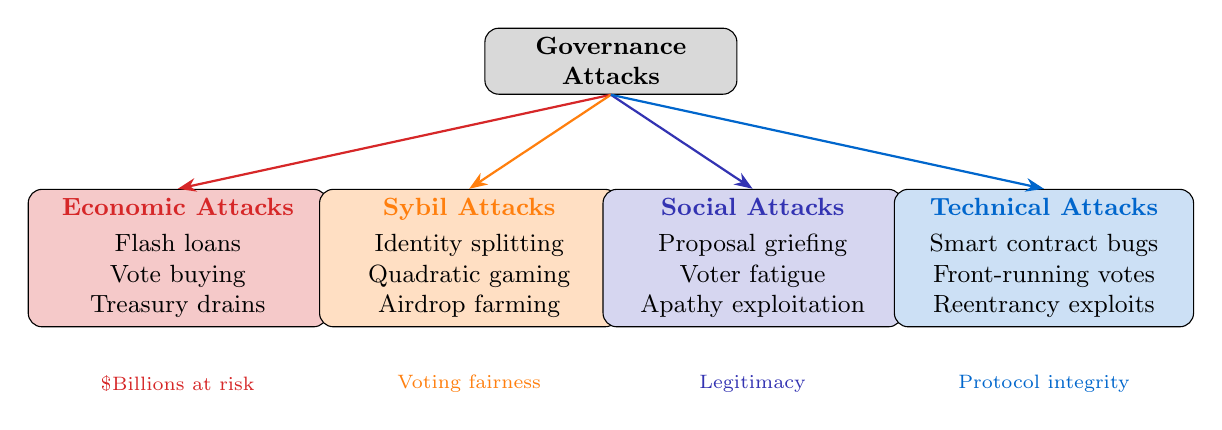
\begin{tikzpicture}[>=Stealth,node distance=1.2cm]
  %% Root node
  \node[draw,fill=mlgray!30,rounded corners=5pt,
        minimum width=3.2cm,minimum height=0.7cm,align=center,font=\small\bfseries]
        (root) at (0,0) {Governance\\Attacks};
  %% Branch 1: Economic
  \node[draw,fill=mlred!25,rounded corners=5pt,
        minimum width=3.8cm,minimum height=1.5cm,align=center,font=\small]
        (econ) at (-5.5,-2.5)
        {\textbf{\textcolor{mlred}{Economic Attacks}}\\[2pt]Flash loans\\Vote buying\\Treasury drains};
  %% Branch 2: Sybil
  \node[draw,fill=mlorange!25,rounded corners=5pt,
        minimum width=3.8cm,minimum height=1.5cm,align=center,font=\small]
        (sybil) at (-1.8,-2.5)
        {\textbf{\textcolor{mlorange}{Sybil Attacks}}\\[2pt]Identity splitting\\Quadratic gaming\\Airdrop farming};
  %% Branch 3: Social
  \node[draw,fill=mlpurple!20,rounded corners=5pt,
        minimum width=3.8cm,minimum height=1.5cm,align=center,font=\small]
        (social) at (1.8,-2.5)
        {\textbf{\textcolor{mlpurple}{Social Attacks}}\\[2pt]Proposal griefing\\Voter fatigue\\Apathy exploitation};
  %% Branch 4: Technical
  \node[draw,fill=mlblue!20,rounded corners=5pt,
        minimum width=3.8cm,minimum height=1.5cm,align=center,font=\small]
        (tech) at (5.5,-2.5)
        {\textbf{\textcolor{mlblue}{Technical Attacks}}\\[2pt]Smart contract bugs\\Front-running votes\\Reentrancy exploits};
  %% Arrows from root
  \draw[->,thick,mlred]    (root.south) -- (econ.north);
  \draw[->,thick,mlorange] (root.south) -- (sybil.north);
  \draw[->,thick,mlpurple] (root.south) -- (social.north);
  \draw[->,thick,mlblue]   (root.south) -- (tech.north);
  %% Impact labels
  \node[align=center,font=\scriptsize,text=mlred]    at (-5.5,-4.1)  {\$Billions at risk};
  \node[align=center,font=\scriptsize,text=mlorange] at (-1.8,-4.1)  {Voting fairness};
  \node[align=center,font=\scriptsize,text=mlpurple] at ( 1.8,-4.1)  {Legitimacy};
  \node[align=center,font=\scriptsize,text=mlblue]   at ( 5.5,-4.1)  {Protocol integrity};
\end{tikzpicture}
\end{center}
\bottomnote{Attack surface grows with protocol value | No single defense covers all attack types --- layered security is mandatory}
\end{frame}

% Frame 41: Flash Loan Governance Attacks
\begin{frame}{Flash Loan Governance Attacks}
\begin{columns}[t]
\column{0.62\textwidth}
\begin{center}
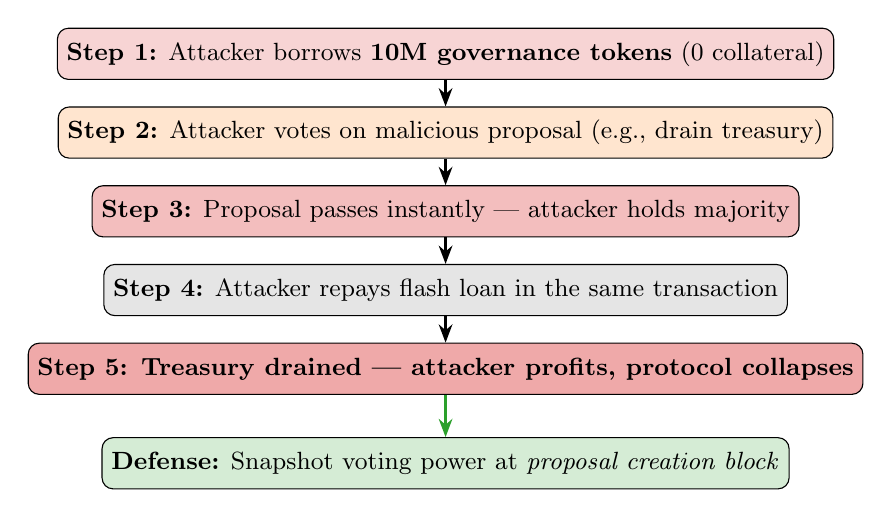
\begin{tikzpicture}[>=Stealth,node distance=0.55cm]
  \node[draw,fill=mlred!20,rounded corners=4pt,
        minimum width=7.2cm,minimum height=0.65cm,align=center,font=\small]
        (s1) at (0, 0)
        {\textbf{Step 1:} Attacker borrows \textbf{10M governance tokens} (0 collateral)};
  \node[draw,fill=mlorange!20,rounded corners=4pt,
        minimum width=7.2cm,minimum height=0.65cm,align=center,font=\small]
        (s2) at (0,-1.0)
        {\textbf{Step 2:} Attacker votes on malicious proposal (e.g., drain treasury)};
  \node[draw,fill=mlred!30,rounded corners=4pt,
        minimum width=7.2cm,minimum height=0.65cm,align=center,font=\small]
        (s3) at (0,-2.0)
        {\textbf{Step 3:} Proposal passes instantly --- attacker holds majority};
  \node[draw,fill=mlgray!20,rounded corners=4pt,
        minimum width=7.2cm,minimum height=0.65cm,align=center,font=\small]
        (s4) at (0,-3.0)
        {\textbf{Step 4:} Attacker repays flash loan in the same transaction};
  \node[draw,fill=mlred!40,rounded corners=4pt,
        minimum width=7.2cm,minimum height=0.65cm,align=center,font=\small\bfseries]
        (s5) at (0,-4.0)
        {\textbf{Step 5:} Treasury drained --- attacker profits, protocol collapses};
  \draw[->,thick] (s1)--(s2);
  \draw[->,thick] (s2)--(s3);
  \draw[->,thick] (s3)--(s4);
  \draw[->,thick] (s4)--(s5);
  \node[draw,fill=mlgreen!20,rounded corners=4pt,
        minimum width=7.2cm,minimum height=0.65cm,align=center,font=\small]
        (def) at (0,-5.2)
        {\textbf{Defense:} Snapshot voting power at \textit{proposal creation block}};
  \draw[->,thick,mlgreen] (s5)--(def);
\end{tikzpicture}
\end{center}
\column{0.35\textwidth}
\begin{block}{Real Example}
\textbf{Beanstalk Farms}\\April 2022\\
\vspace{2pt}
\begin{itemize}\small
  \item Attacker borrowed \$1B in flash loan
  \item Passed emergency BIP-18 proposal
  \item Drained \$182M from protocol
  \item All in a \textbf{single transaction}
\end{itemize}
\end{block}
\vspace{4pt}
\begin{block}{Key Insight}
\small Flash loans make anyone temporarily the largest token holder --- voting power must be measured \textit{before} the loan is taken.
\end{block}
\end{columns}
\bottomnote{Flash loan attacks exploit the atomic nature of blockchain transactions | Prevention: ERC20Votes with block-number checkpoints}
\end{frame}

% Frame 42: Governance Attack Scenario [fragile] -- CODE FRAME 4
\begin{frame}[fragile]{Flash Loan Governance Attack}
\begin{columns}[t]
\column{0.5\textwidth}
\begin{lstlisting}[language=Solidity,caption=Attack Contract]
// Flash Loan Governance Attack
contract GovernanceAttack {
    function attack(
        address lender,
        address governor,
        uint256 proposalId
    ) external {
        // Step 1: Borrow tokens
        IFlashLender(lender)
            .flashLoan(10_000_000e18);

        // Step 2: Vote with
        //         borrowed tokens
        IGovernor(governor)
            .castVote(
                proposalId,
                1 // FOR
            );

        // Step 3: Repay in same tx
        IERC20(token).transfer(
            lender, 10_000_000e18);
    }
}
\end{lstlisting}
\column{0.47\textwidth}
\begin{block}{Why It Works}
\small Voting power checked \textbf{at call time} --- attacker holds 10M tokens when \texttt{castVote()} executes, even though they will be returned moments later.
\end{block}
\vspace{4pt}
\begin{block}{Defenses}
\begin{itemize}\small
  \item \textbf{ERC20Votes}: stores voting power at each block with checkpoints
  \item \textbf{Snapshot}: governance reads balance at \textit{proposal creation block}, not current block
  \item \textbf{Compound GovernorBravo}: uses \texttt{getPriorVotes(account, block-1)} to prevent same-block manipulation
\end{itemize}
\end{block}
\end{columns}
\bottomnote{Code Frame 4 | The fix is elegant: measure who had tokens \textit{before} the proposal, not during the vote}
\end{frame}

% Frame 43: Vote Buying & Bribery
\begin{frame}{Vote Buying \& Bribery}
\begin{columns}[t]
\column{0.55\textwidth}
\begin{center}
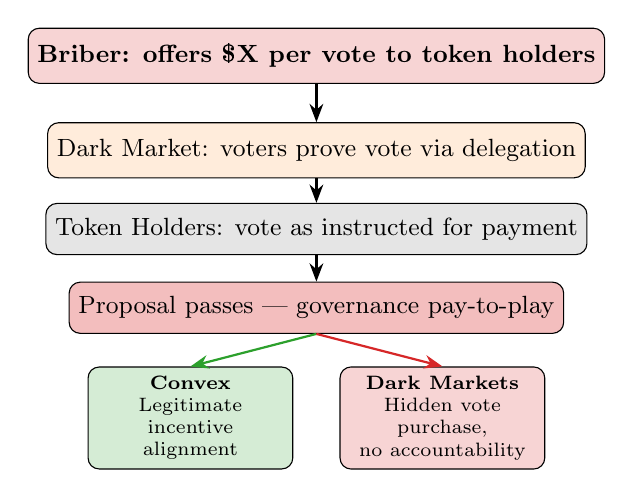
\begin{tikzpicture}[>=Stealth,node distance=0.7cm]
  \node[draw,fill=mlred!20,rounded corners=4pt,
        minimum width=5.8cm,minimum height=0.7cm,align=center,font=\small\bfseries]
        (briber) at (0,0) {Briber: offers \$X per vote to token holders};
  \node[draw,fill=mlorange!15,rounded corners=4pt,
        minimum width=5.8cm,minimum height=0.7cm,align=center,font=\small]
        (mkt) at (0,-1.2) {Dark Market: voters prove vote via delegation};
  \node[draw,fill=mlgray!20,rounded corners=4pt,
        minimum width=5.8cm,minimum height=0.65cm,align=center,font=\small]
        (tok) at (0,-2.2) {Token Holders: vote as instructed for payment};
  \node[draw,fill=mlred!30,rounded corners=4pt,
        minimum width=5.8cm,minimum height=0.65cm,align=center,font=\small]
        (result) at (0,-3.2) {Proposal passes --- governance pay-to-play};
  \draw[->,thick] (briber)--(mkt);
  \draw[->,thick] (mkt)--(tok);
  \draw[->,thick] (tok)--(result);
  %% Comparison nodes
  \node[draw,fill=mlgreen!20,rounded corners=4pt,
        minimum width=2.6cm,minimum height=1.2cm,align=center,font=\scriptsize]
        (conv) at (-1.6,-4.6)
        {\textbf{Convex}\\Legitimate\\incentive\\alignment};
  \node[draw,fill=mlred!20,rounded corners=4pt,
        minimum width=2.6cm,minimum height=1.2cm,align=center,font=\scriptsize]
        (dark) at (1.6,-4.6)
        {\textbf{Dark Markets}\\Hidden vote\\purchase,\\no accountability};
  \draw[->,thick,mlgreen] (result.south)--(conv.north);
  \draw[->,thick,mlred]   (result.south)--(dark.north);
\end{tikzpicture}
\end{center}
\column{0.42\textwidth}
\begin{block}{The ``Governance is a Market'' Thesis}
\small Governance votes have financial value. If a protocol controls \$1B in assets, voting rights are worth significant money --- creating natural bribery incentives.
\end{block}
\vspace{4pt}
\begin{block}{Defenses}
\begin{itemize}\small
  \item \textbf{Vote Privacy (MACI)}: Minimum Anti-Collusion Infrastructure --- voters can change votes privately, making bribes unverifiable
  \item \textbf{Shielded Voting}: votes hidden until voting period closes
  \item \textbf{Commit-Reveal}: two-phase voting to prevent last-minute coordination
\end{itemize}
\end{block}
\end{columns}
\bottomnote{Vote buying is rational if the governance asset is worth more than the bribe cost | MACI offers cryptographic bribery resistance}
\end{frame}

% Frame 44: Sybil Attacks on Governance
\begin{frame}{Sybil Attacks on Governance}
\begin{columns}[t]
\column{0.55\textwidth}
\begin{center}
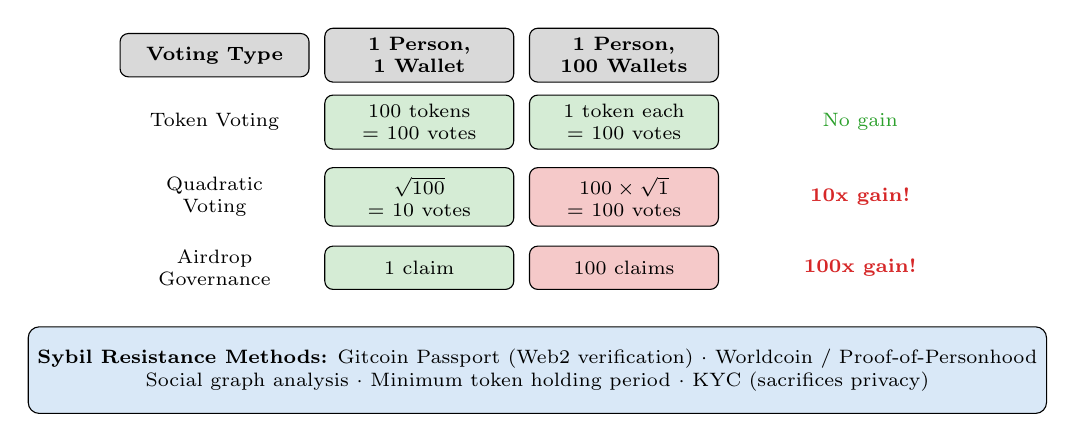
\begin{tikzpicture}[>=Stealth]
  %% Header row
  \node[draw,fill=mlgray!30,rounded corners=3pt,
        minimum width=2.4cm,minimum height=0.55cm,align=center,font=\scriptsize\bfseries]
        at (-2.4,0) {Voting Type};
  \node[draw,fill=mlgray!30,rounded corners=3pt,
        minimum width=2.4cm,minimum height=0.55cm,align=center,font=\scriptsize\bfseries]
        at (0.2,0) {1 Person,\\1 Wallet};
  \node[draw,fill=mlgray!30,rounded corners=3pt,
        minimum width=2.4cm,minimum height=0.55cm,align=center,font=\scriptsize\bfseries]
        at (2.8,0) {1 Person,\\100 Wallets};
  %% Row 1: Token Voting
  \node[align=center,font=\scriptsize] at (-2.4,-0.85) {Token Voting};
  \node[draw,fill=mlgreen!20,rounded corners=3pt,
        minimum width=2.4cm,minimum height=0.55cm,align=center,font=\scriptsize]
        at (0.2,-0.85) {100 tokens\\= 100 votes};
  \node[draw,fill=mlgreen!20,rounded corners=3pt,
        minimum width=2.4cm,minimum height=0.55cm,align=center,font=\scriptsize]
        at (2.8,-0.85) {1 token each\\= 100 votes};
  \node[align=center,font=\scriptsize,text=mlgreen] at (5.8,-0.85) {No gain};
  %% Row 2: Quadratic Voting
  \node[align=center,font=\scriptsize] at (-2.4,-1.8) {Quadratic\\Voting};
  \node[draw,fill=mlgreen!20,rounded corners=3pt,
        minimum width=2.4cm,minimum height=0.55cm,align=center,font=\scriptsize]
        at (0.2,-1.8) {$\sqrt{100}$\\= 10 votes};
  \node[draw,fill=mlred!25,rounded corners=3pt,
        minimum width=2.4cm,minimum height=0.55cm,align=center,font=\scriptsize]
        at (2.8,-1.8) {$100\times\sqrt{1}$\\= 100 votes};
  \node[align=center,font=\scriptsize,text=mlred] at (5.8,-1.8) {\textbf{10x gain!}};
  %% Row 3: Airdrop
  \node[align=center,font=\scriptsize] at (-2.4,-2.7) {Airdrop\\Governance};
  \node[draw,fill=mlgreen!20,rounded corners=3pt,
        minimum width=2.4cm,minimum height=0.55cm,align=center,font=\scriptsize]
        at (0.2,-2.7) {1 claim};
  \node[draw,fill=mlred!25,rounded corners=3pt,
        minimum width=2.4cm,minimum height=0.55cm,align=center,font=\scriptsize]
        at (2.8,-2.7) {100 claims};
  \node[align=center,font=\scriptsize,text=mlred] at (5.8,-2.7) {\textbf{100x gain!}};
  %% Sybil resistance methods
  \node[draw,fill=mlblue!15,rounded corners=4pt,
        minimum width=8.6cm,minimum height=1.1cm,align=center,font=\scriptsize]
        at (1.7,-4.0)
        {\textbf{Sybil Resistance Methods:}
        Gitcoin Passport (Web2 verification) $\cdot$
        Worldcoin / Proof-of-Personhood\\
        Social graph analysis $\cdot$
        Minimum token holding period $\cdot$
        KYC (sacrifices privacy)};
\end{tikzpicture}
\end{center}
\column{0.42\textwidth}
\begin{block}{The Core Tradeoff}
\small \textbf{Sybil resistance} requires identifying unique humans --- which conflicts with the \textbf{pseudonymity} that blockchain users value.
\end{block}
\vspace{4pt}
\begin{block}{No Perfect Solution}
\begin{itemize}\small
  \item KYC: effective but centralizing
  \item Proof-of-personhood: promising but experimental (Worldcoin controversy)
  \item Social graphs: gameable over time
  \item Holding periods: reduce but don't eliminate Sybil advantage
\end{itemize}
\end{block}
\end{columns}
\bottomnote{Sybil attacks are especially dangerous for quadratic voting systems | Privacy vs. Sybil-resistance remains an open research problem}
\end{frame}

% Frame 45: The DAO Hack 2016
\begin{frame}{The DAO Hack (2016): A Watershed Moment}
\begin{center}
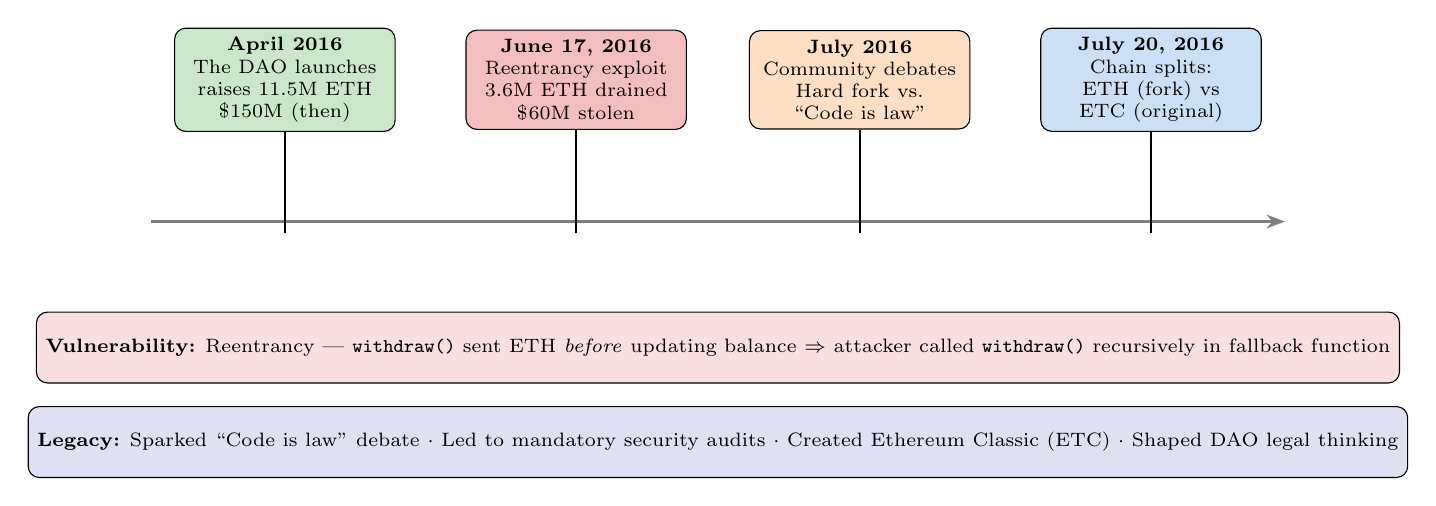
\begin{tikzpicture}[>=Stealth]
  %% Timeline bar
  \draw[thick,mlgray,->] (-7.2,0) -- (7.2,0);
  %% Events
  \node[draw,fill=mlgreen!25,rounded corners=4pt,
        minimum width=2.8cm,minimum height=1.1cm,align=center,font=\scriptsize]
        (e1) at (-5.5, 1.8)
        {\textbf{April 2016}\\The DAO launches\\raises 11.5M ETH\\\$150M (then)};
  \node[draw,fill=mlred!30,rounded corners=4pt,
        minimum width=2.8cm,minimum height=1.1cm,align=center,font=\scriptsize]
        (e2) at (-1.8, 1.8)
        {\textbf{June 17, 2016}\\Reentrancy exploit\\3.6M ETH drained\\\$60M stolen};
  \node[draw,fill=mlorange!25,rounded corners=4pt,
        minimum width=2.8cm,minimum height=1.1cm,align=center,font=\scriptsize]
        (e3) at (1.8, 1.8)
        {\textbf{July 2016}\\Community debates\\Hard fork vs.\\``Code is law''};
  \node[draw,fill=mlblue!20,rounded corners=4pt,
        minimum width=2.8cm,minimum height=1.1cm,align=center,font=\scriptsize]
        (e4) at (5.5, 1.8)
        {\textbf{July 20, 2016}\\Chain splits:\\ETH (fork) vs\\ETC (original)};
  %% Connectors to timeline
  \draw[thick] (-5.5,0) -- (e1.south);
  \draw[thick] (-1.8,0) -- (e2.south);
  \draw[thick] ( 1.8,0) -- (e3.south);
  \draw[thick] ( 5.5,0) -- (e4.south);
  %% Tick marks
  \foreach \x in {-5.5,-1.8,1.8,5.5}
    \draw[thick] (\x,-0.15)--(\x,0.15);
  %% Technical box below
  \node[draw,fill=mlred!15,rounded corners=4pt,
        minimum width=14cm,minimum height=0.9cm,align=center,font=\scriptsize]
        at (0,-1.6)
        {\textbf{Vulnerability:} Reentrancy --- \texttt{withdraw()} sent ETH \textit{before} updating balance $\Rightarrow$ attacker called \texttt{withdraw()} recursively in fallback function};
  \node[draw,fill=mlpurple!15,rounded corners=4pt,
        minimum width=14cm,minimum height=0.9cm,align=center,font=\scriptsize]
        at (0,-2.8)
        {\textbf{Legacy:} Sparked ``Code is law'' debate $\cdot$ Led to mandatory security audits $\cdot$ Created Ethereum Classic (ETC) $\cdot$ Shaped DAO legal thinking};
\end{tikzpicture}
\end{center}
\bottomnote{The DAO hack was the first major test of blockchain governance under crisis | The fork proved that human consensus can override ``immutable'' code}
\end{frame}

% Frame 46: Defensive Mechanisms
\begin{frame}{Defensive Mechanisms: Defense-in-Depth}
\begin{columns}[t]
\column{0.58\textwidth}
\begin{center}
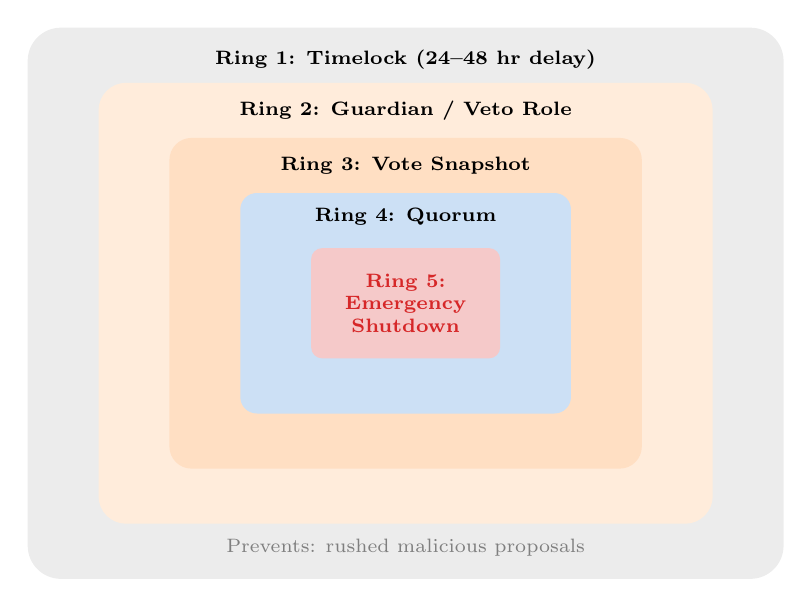
\begin{tikzpicture}
  %% Concentric rings (outermost to innermost)
  \fill[mlgray!15,rounded corners=12pt] (-4.8,-3.5) rectangle (4.8,3.5);
  \fill[mlorange!15,rounded corners=10pt] (-3.9,-2.8) rectangle (3.9,2.8);
  \fill[mlorange!25,rounded corners=8pt] (-3.0,-2.1) rectangle (3.0,2.1);
  \fill[mlblue!20,rounded corners=6pt] (-2.1,-1.4) rectangle (2.1,1.4);
  \fill[mlred!25,rounded corners=4pt] (-1.2,-0.7) rectangle (1.2,0.7);
  %% Labels on rings
  \node[align=center,font=\scriptsize\bfseries] at (0, 3.1) {Ring 1: Timelock (24--48 hr delay)};
  \node[align=center,font=\scriptsize,text=mlgray] at (0,-3.1) {Prevents: rushed malicious proposals};
  \node[align=center,font=\scriptsize\bfseries] at (0, 2.45) {Ring 2: Guardian / Veto Role};
  \node[align=center,font=\scriptsize\bfseries] at (0, 1.75) {Ring 3: Vote Snapshot};
  \node[align=center,font=\scriptsize\bfseries] at (0, 1.1) {Ring 4: Quorum};
  \node[align=center,font=\scriptsize\bfseries,text=mlred] at (0, 0) {Ring 5:\\Emergency\\Shutdown};
\end{tikzpicture}
\end{center}
\column{0.40\textwidth}
\begin{itemize}\small
  \item \textbf{Ring 1 --- Timelock:} 24--48 hour delay between vote passing and execution; users can exit before harmful change takes effect
  \item \textbf{Ring 2 --- Guardian:} Multisig committee can cancel proposals during timelock; sacrifices some decentralization for safety
  \item \textbf{Ring 3 --- Snapshot:} Voting power measured at proposal creation block; defeats flash loan attacks
  \item \textbf{Ring 4 --- Quorum:} Minimum participation required; prevents minority capture with abstaining majority
  \item \textbf{Ring 5 --- Emergency Shutdown:} Circuit breaker pauses protocol; last resort against active exploits
\end{itemize}
\end{columns}
\bottomnote{No single mechanism is sufficient | Layer all five rings for robust governance security}
\end{frame}

% Frame 47: Governance Minimization
\begin{frame}{Governance Minimization}
\begin{columns}[t]
\column{0.42\textwidth}
\begin{block}{Philosophy}
\small Reduce the attack surface by reducing what governance can control. The safest governance decision is one that \textbf{does not need to be made}.
\end{block}
\vspace{4pt}
\begin{itemize}\small
  \item \textbf{Immutable code} cannot be governance-attacked
  \item \textbf{Progressive decentralization}: gradually hand control to the DAO as trust is established
  \item \textbf{Uniswap v3}: minimal governance --- only fee switch and grant programs
  \item \textbf{MakerDAO}: extensive governance --- hundreds of decisions per year, higher risk surface
\end{itemize}
\column{0.55\textwidth}
\begin{center}
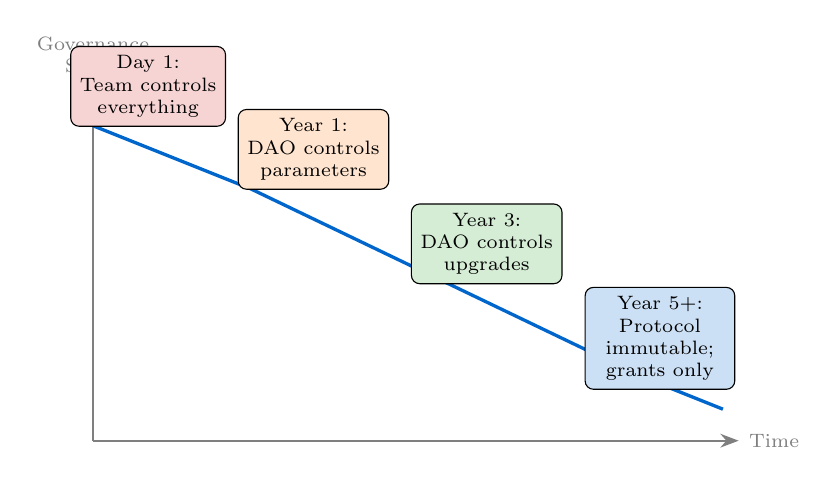
\begin{tikzpicture}[>=Stealth]
  \draw[thick,->,mlgray] (0,0) -- (8.2,0) node[right,font=\scriptsize] {Time};
  \draw[thick,->,mlgray] (0,0) -- (0,4.5) node[above,font=\scriptsize,align=center] {Governance\\Scope};
  %% Declining governance scope line
  \draw[very thick,mlblue] (0,4.0) -- (2.0,3.2) -- (4.5,2.0) -- (7.0,0.8) -- (8.0,0.4);
  %% Stage markers
  \node[draw,fill=mlred!20,rounded corners=3pt,
        minimum width=1.8cm,minimum height=0.7cm,align=center,font=\scriptsize]
        at (0.7,4.5) {Day 1:\\Team controls\\everything};
  \node[draw,fill=mlorange!20,rounded corners=3pt,
        minimum width=1.8cm,minimum height=0.7cm,align=center,font=\scriptsize]
        at (2.8,3.7) {Year 1:\\DAO controls\\parameters};
  \node[draw,fill=mlgreen!20,rounded corners=3pt,
        minimum width=1.8cm,minimum height=0.7cm,align=center,font=\scriptsize]
        at (5.0,2.5) {Year 3:\\DAO controls\\upgrades};
  \node[draw,fill=mlblue!20,rounded corners=3pt,
        minimum width=1.9cm,minimum height=0.75cm,align=center,font=\scriptsize]
        at (7.2,1.3) {Year 5+:\\Protocol\\immutable;\\ grants only};
\end{tikzpicture}
\end{center}
\end{columns}
\bottomnote{The safest governance decision is one that doesn't need to be made --- immutable code can't be attacked via governance}
\end{frame}

% Frame 48: Section 4 Summary
\begin{frame}{Section 4 Summary: Governance Security}
\begin{center}
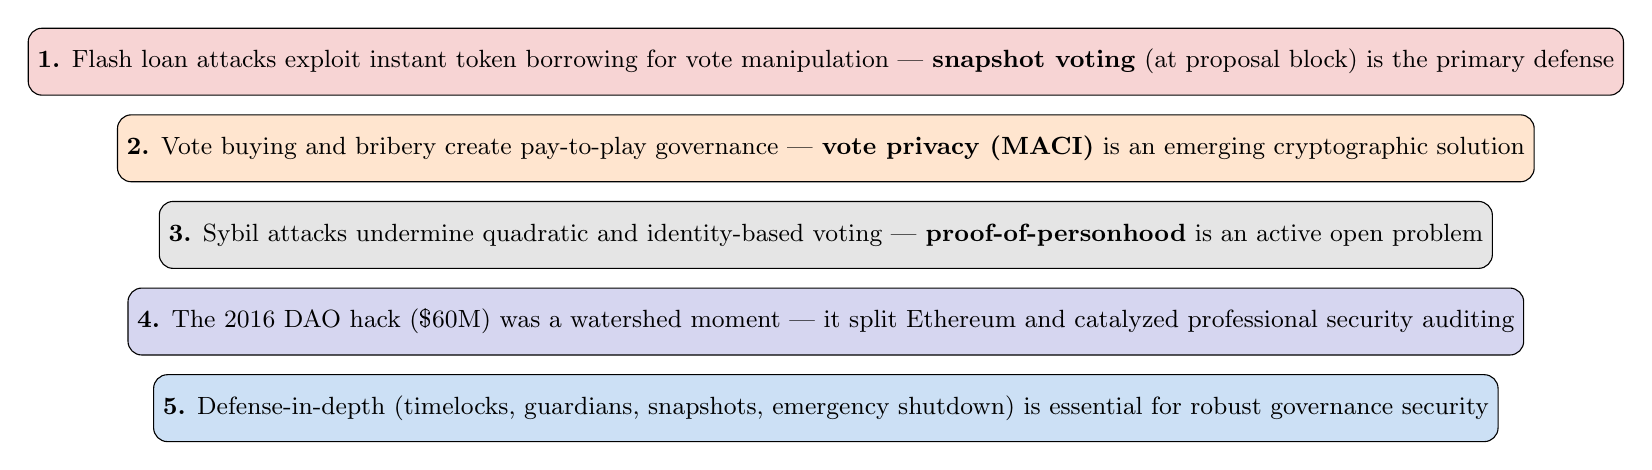
\begin{tikzpicture}
  \node[draw,fill=mlred!20,rounded corners=5pt,
        minimum width=14.5cm,minimum height=0.85cm,align=center,font=\small]
        at (0, 2.4)
        {\textbf{1.} Flash loan attacks exploit instant token borrowing for vote manipulation --- \textbf{snapshot voting} (at proposal block) is the primary defense};
  \node[draw,fill=mlorange!20,rounded corners=5pt,
        minimum width=14.5cm,minimum height=0.85cm,align=center,font=\small]
        at (0, 1.3)
        {\textbf{2.} Vote buying and bribery create pay-to-play governance --- \textbf{vote privacy (MACI)} is an emerging cryptographic solution};
  \node[draw,fill=mlgray!20,rounded corners=5pt,
        minimum width=14.5cm,minimum height=0.85cm,align=center,font=\small]
        at (0, 0.2)
        {\textbf{3.} Sybil attacks undermine quadratic and identity-based voting --- \textbf{proof-of-personhood} is an active open problem};
  \node[draw,fill=mlpurple!20,rounded corners=5pt,
        minimum width=14.5cm,minimum height=0.85cm,align=center,font=\small]
        at (0,-0.9)
        {\textbf{4.} The 2016 DAO hack (\$60M) was a watershed moment --- it split Ethereum and catalyzed professional security auditing};
  \node[draw,fill=mlblue!20,rounded corners=5pt,
        minimum width=14.5cm,minimum height=0.85cm,align=center,font=\small]
        at (0,-2.0)
        {\textbf{5.} Defense-in-depth (timelocks, guardians, snapshots, emergency shutdown) is essential for robust governance security};
\end{tikzpicture}
\vspace{4mm}

\begin{tikzpicture}
  \node[draw,fill=mlpurple,text=white,rounded corners=6pt,
        minimum width=10cm,minimum height=0.8cm,align=center,font=\small\bfseries]
        at (0,0) {Next: Section 5 --- Real-World DAOs \& Future of Governance};
\end{tikzpicture}
\end{center}
\bottomnote{Section 4 complete | Key insight: layered defenses and governance minimization are the two most powerful security strategies}
\end{frame}

%% ============================================================
%% SECTION 5: Real-World DAOs & Future of Governance
%% ============================================================
\section{Case Studies \& Future}

% Frame 49: Section 5 Divider
\begin{frame}
\begin{center}
\begin{beamercolorbox}[sep=12pt,center,rounded=true,shadow=true]{palette quaternary}
{\Large\bfseries Section 5: Real-World DAOs \& Future of Governance}\\[6pt]
{\normalsize Case studies, participation challenges, and the road ahead}
\end{beamercolorbox}

\vspace{4mm}
\begin{columns}[t]
\column{0.5\textwidth}
\begin{block}{What You Will Learn}
\begin{itemize}
  \item MakerDAO, Uniswap, and Aave governance case studies
  \item Governance participation rates and voter apathy
\end{itemize}
\end{block}
\column{0.5\textwidth}
\begin{block}{}
\begin{itemize}
  \item Legal frameworks for DAOs by jurisdiction
  \item The future of decentralized governance
\end{itemize}
\end{block}
\end{columns}
\end{center}
\bottomnote{Section 5 of 5 | Real-world DAOs prove both the promise and the hard problems of decentralized governance}
\end{frame}

% Frame 50: MakerDAO Governance
\begin{frame}{MakerDAO Governance}
\begin{columns}[t]
\column{0.45\textwidth}
\begin{block}{Structure}
\begin{itemize}\small
  \item \textbf{MKR token} holders govern the \textbf{DAI} stablecoin system
  \item Key parameters: stability fees, collateral ratios, DSR (DAI Savings Rate)
  \item \textbf{Hat system}: continuous approval voting --- proposal with most MKR locked becomes the ``hat'' and is executable
  \item Hundreds of governance decisions per year
\end{itemize}
\end{block}
\vspace{4pt}
\begin{block}{Endgame Plan}
\small SubDAOs, MetaDAOs, real-world asset integration --- MakerDAO evolving toward modular governance with specialized sub-units each managing a vertical.
\end{block}
\column{0.52\textwidth}
\begin{center}
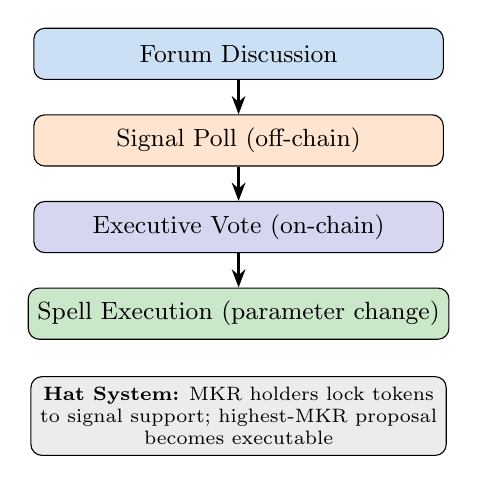
\begin{tikzpicture}[>=Stealth,node distance=0.9cm]
  \node[draw,fill=mlblue!20,rounded corners=4pt,
        minimum width=5.2cm,minimum height=0.65cm,align=center,font=\small]
        (forum) at (0,0) {Forum Discussion};
  \node[draw,fill=mlorange!20,rounded corners=4pt,
        minimum width=5.2cm,minimum height=0.65cm,align=center,font=\small]
        (poll) at (0,-1.1) {Signal Poll (off-chain)};
  \node[draw,fill=mlpurple!20,rounded corners=4pt,
        minimum width=5.2cm,minimum height=0.65cm,align=center,font=\small]
        (exec) at (0,-2.2) {Executive Vote (on-chain)};
  \node[draw,fill=mlgreen!25,rounded corners=4pt,
        minimum width=5.2cm,minimum height=0.65cm,align=center,font=\small]
        (spell) at (0,-3.3) {Spell Execution (parameter change)};
  \draw[->,thick] (forum)--(poll);
  \draw[->,thick] (poll)--(exec);
  \draw[->,thick] (exec)--(spell);
  \node[draw,fill=mlgray!15,rounded corners=4pt,
        minimum width=5.2cm,minimum height=1.0cm,align=center,font=\scriptsize]
        at (0,-4.6)
        {\textbf{Hat System:} MKR holders lock tokens\\ to signal support; highest-MKR proposal\\ becomes executable};
\end{tikzpicture}
\end{center}
\end{columns}
\bottomnote{MakerDAO governs the \$5B+ DAI ecosystem | Complexity concern: high governance overhead risks voter fatigue and plutocratic capture}
\end{frame}

% Frame 51: Uniswap & Aave Governance
\begin{frame}{Uniswap \& Aave Governance}
\begin{columns}[t]
\column{0.48\textwidth}
\begin{block}{Uniswap Governance}
\begin{itemize}\small
  \item \textbf{Token:} UNI (1B total supply)
  \item \textbf{System:} Governor Bravo (OpenZeppelin)
  \item \textbf{Quorum:} 4\% of supply ($\approx$40M UNI)
  \item \textbf{Voting period:} 7 days
  \item \textbf{Timelock:} 2-day delay
  \item \textbf{Key debates:} Fee switch (protocol revenue), BSL license exceptions, deployment on new chains
  \item \textbf{Challenge:} Large holders dominate; retail rarely reaches proposal threshold (2.5M UNI to propose)
\end{itemize}
\end{block}
\column{0.48\textwidth}
\begin{block}{Aave Governance}
\begin{itemize}\small
  \item \textbf{Token:} AAVE + stkAAVE (staked)
  \item \textbf{System:} Governance v3 (cross-chain)
  \item \textbf{Safety Module:} stkAAVE holders backstop protocol losses
  \item \textbf{Risk DAO:} Specialized committee for risk parameter updates
  \item \textbf{Cross-chain:} Governance on Ethereum controls deployments on Polygon, Avalanche, Optimism
  \item \textbf{Key decisions:} New asset listings, interest rate models, protocol upgrades
\end{itemize}
\end{block}
\end{columns}
\vspace{2pt}
\begin{center}
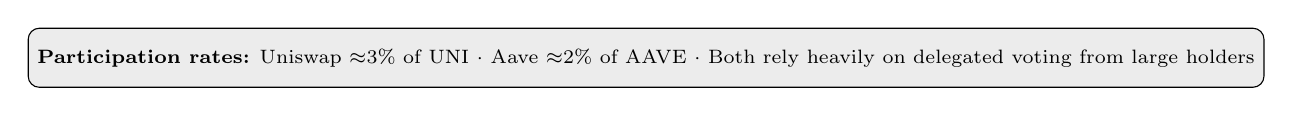
\begin{tikzpicture}
  \node[draw,fill=mlgray!15,rounded corners=4pt,
        minimum width=14cm,minimum height=0.75cm,align=center,font=\scriptsize]
        at (0,0)
        {\textbf{Participation rates:} Uniswap $\approx$3\% of UNI $\cdot$ Aave $\approx$2\% of AAVE $\cdot$ Both rely heavily on delegated voting from large holders};
\end{tikzpicture}
\end{center}
\bottomnote{Both protocols show: good governance tooling exists, but participation remains the unsolved challenge}
\end{frame}

% Frame 52: Governance Participation Crisis
\begin{frame}{Governance Participation Crisis}
\begin{columns}[t]
\column{0.58\textwidth}
\begin{center}
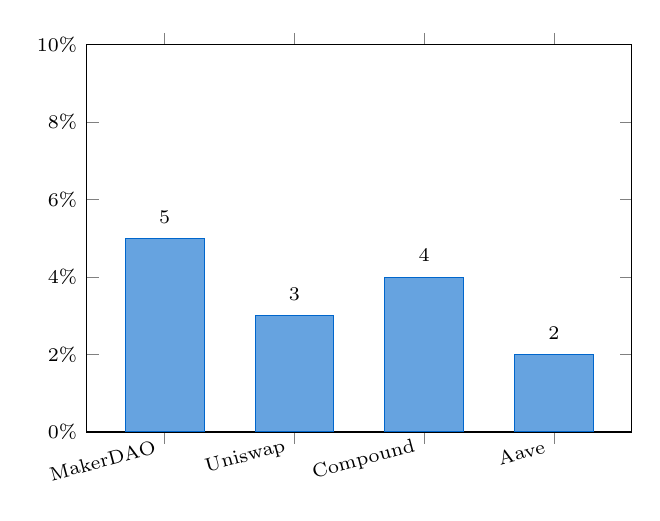
\begin{tikzpicture}
\begin{axis}[
  width=8.5cm, height=6.5cm,
  ybar,
  bar width=1.0cm,
  symbolic x coords={MakerDAO,Uniswap,Compound,Aave},
  xtick=data,
  xticklabel style={font=\scriptsize,rotate=15,anchor=east},
  ymin=0, ymax=10,
  ytick={0,2,4,6,8,10},
  yticklabel={\pgfmathprintnumber{\tick}\%},
  yticklabel style={font=\scriptsize},
  ylabel style={font=\scriptsize},
  title style={font=\small},
  enlarge x limits=0.2,
  nodes near coords,
  nodes near coords style={font=\scriptsize},
  every node near coord/.append style={yshift=2pt},
]
\addplot[fill=mlblue!60,draw=mlblue] coordinates {
  (MakerDAO,5) (Uniswap,3) (Compound,4) (Aave,2)
};
\end{axis}
\end{tikzpicture}
\end{center}
\column{0.40\textwidth}
\begin{block}{Root Causes}
\begin{itemize}\small
  \item \textbf{Voter fatigue:} too many proposals, too little time
  \item \textbf{Gas costs:} voting on-chain costs \$5--\$50 per vote
  \item \textbf{Complexity:} proposals require deep protocol knowledge
  \item \textbf{Rational ignorance:} small token holders' votes rarely decisive
\end{itemize}
\end{block}
\vspace{4pt}
\begin{block}{Solutions}
\begin{itemize}\small
  \item Delegation to active representatives
  \item Gasless voting (Snapshot off-chain)
  \item Governance mining (rewards for voting)
  \item Simplified proposal summaries
\end{itemize}
\end{block}
\end{columns}
\bottomnote{Avg. turnout below 5\% means a motivated minority can dominate governance | Low participation is a systemic vulnerability, not just inconvenience}
\end{frame}

% Frame 53: DAO Legal Frameworks
\begin{frame}{DAO Legal Frameworks}
\begin{center}
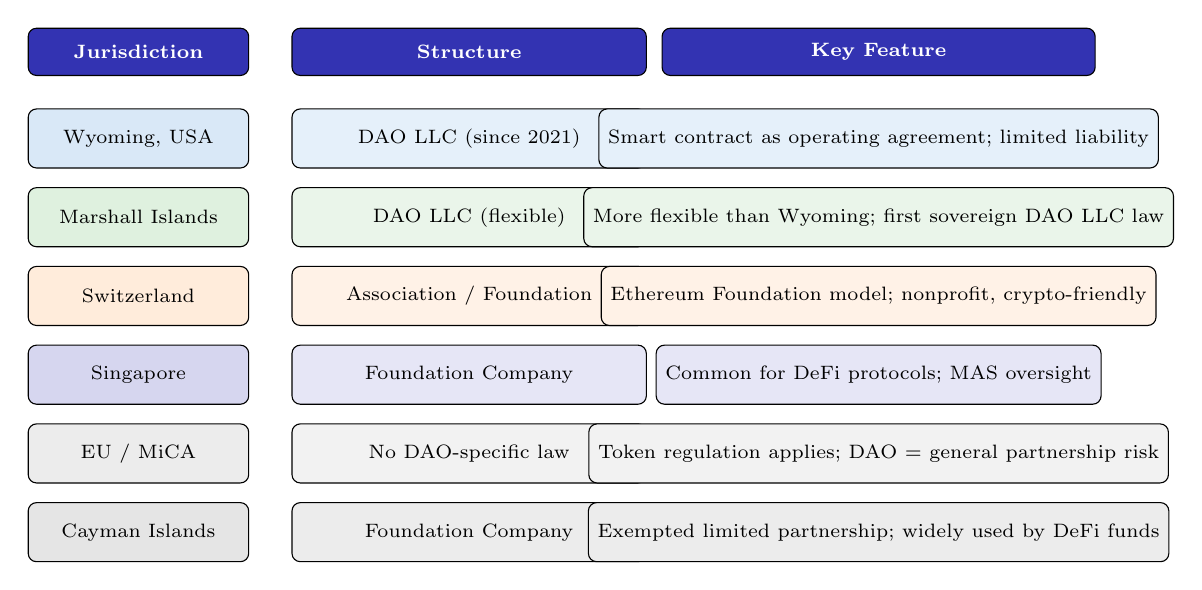
\begin{tikzpicture}
  %% Column headers
  \node[draw,fill=mlpurple,text=white,rounded corners=3pt,
        minimum width=2.8cm,minimum height=0.6cm,align=center,font=\scriptsize\bfseries]
        at (-5.2,2.2) {Jurisdiction};
  \node[draw,fill=mlpurple,text=white,rounded corners=3pt,
        minimum width=4.5cm,minimum height=0.6cm,align=center,font=\scriptsize\bfseries]
        at (-1.0,2.2) {Structure};
  \node[draw,fill=mlpurple,text=white,rounded corners=3pt,
        minimum width=5.5cm,minimum height=0.6cm,align=center,font=\scriptsize\bfseries]
        at (4.2,2.2) {Key Feature};
  %% Row 1
  \node[draw,fill=mlblue!15,rounded corners=3pt,
        minimum width=2.8cm,minimum height=0.75cm,align=center,font=\scriptsize]
        at (-5.2, 1.1) {Wyoming, USA};
  \node[draw,fill=mlblue!10,rounded corners=3pt,
        minimum width=4.5cm,minimum height=0.75cm,align=center,font=\scriptsize]
        at (-1.0, 1.1) {DAO LLC (since 2021)};
  \node[draw,fill=mlblue!10,rounded corners=3pt,
        minimum width=5.5cm,minimum height=0.75cm,align=center,font=\scriptsize]
        at (4.2, 1.1) {Smart contract as operating agreement; limited liability};
  %% Row 2
  \node[draw,fill=mlgreen!15,rounded corners=3pt,
        minimum width=2.8cm,minimum height=0.75cm,align=center,font=\scriptsize]
        at (-5.2, 0.1) {Marshall Islands};
  \node[draw,fill=mlgreen!10,rounded corners=3pt,
        minimum width=4.5cm,minimum height=0.75cm,align=center,font=\scriptsize]
        at (-1.0, 0.1) {DAO LLC (flexible)};
  \node[draw,fill=mlgreen!10,rounded corners=3pt,
        minimum width=5.5cm,minimum height=0.75cm,align=center,font=\scriptsize]
        at (4.2, 0.1) {More flexible than Wyoming; first sovereign DAO LLC law};
  %% Row 3
  \node[draw,fill=mlorange!15,rounded corners=3pt,
        minimum width=2.8cm,minimum height=0.75cm,align=center,font=\scriptsize]
        at (-5.2,-0.9) {Switzerland};
  \node[draw,fill=mlorange!10,rounded corners=3pt,
        minimum width=4.5cm,minimum height=0.75cm,align=center,font=\scriptsize]
        at (-1.0,-0.9) {Association / Foundation};
  \node[draw,fill=mlorange!10,rounded corners=3pt,
        minimum width=5.5cm,minimum height=0.75cm,align=center,font=\scriptsize]
        at (4.2,-0.9) {Ethereum Foundation model; nonprofit, crypto-friendly};
  %% Row 4
  \node[draw,fill=mllavender!50,rounded corners=3pt,
        minimum width=2.8cm,minimum height=0.75cm,align=center,font=\scriptsize]
        at (-5.2,-1.9) {Singapore};
  \node[draw,fill=mllavender!30,rounded corners=3pt,
        minimum width=4.5cm,minimum height=0.75cm,align=center,font=\scriptsize]
        at (-1.0,-1.9) {Foundation Company};
  \node[draw,fill=mllavender!30,rounded corners=3pt,
        minimum width=5.5cm,minimum height=0.75cm,align=center,font=\scriptsize]
        at (4.2,-1.9) {Common for DeFi protocols; MAS oversight};
  %% Row 5
  \node[draw,fill=mlgray!15,rounded corners=3pt,
        minimum width=2.8cm,minimum height=0.75cm,align=center,font=\scriptsize]
        at (-5.2,-2.9) {EU / MiCA};
  \node[draw,fill=mlgray!10,rounded corners=3pt,
        minimum width=4.5cm,minimum height=0.75cm,align=center,font=\scriptsize]
        at (-1.0,-2.9) {No DAO-specific law};
  \node[draw,fill=mlgray!10,rounded corners=3pt,
        minimum width=5.5cm,minimum height=0.75cm,align=center,font=\scriptsize]
        at (4.2,-2.9) {Token regulation applies; DAO = general partnership risk};
  %% Row 6
  \node[draw,fill=mlgray!20,rounded corners=3pt,
        minimum width=2.8cm,minimum height=0.75cm,align=center,font=\scriptsize]
        at (-5.2,-3.9) {Cayman Islands};
  \node[draw,fill=mlgray!15,rounded corners=3pt,
        minimum width=4.5cm,minimum height=0.75cm,align=center,font=\scriptsize]
        at (-1.0,-3.9) {Foundation Company};
  \node[draw,fill=mlgray!15,rounded corners=3pt,
        minimum width=5.5cm,minimum height=0.75cm,align=center,font=\scriptsize]
        at (4.2,-3.9) {Exempted limited partnership; widely used by DeFi funds};
\end{tikzpicture}
\end{center}
\bottomnote{Key risk: Without a legal wrapper, a DAO may be a general partnership --- Ooki DAO case (CFTC) held token voters liable as partners}
\end{frame}

% Frame 54: The Future of DAO Governance
\begin{frame}{The Future of DAO Governance}
\begin{center}
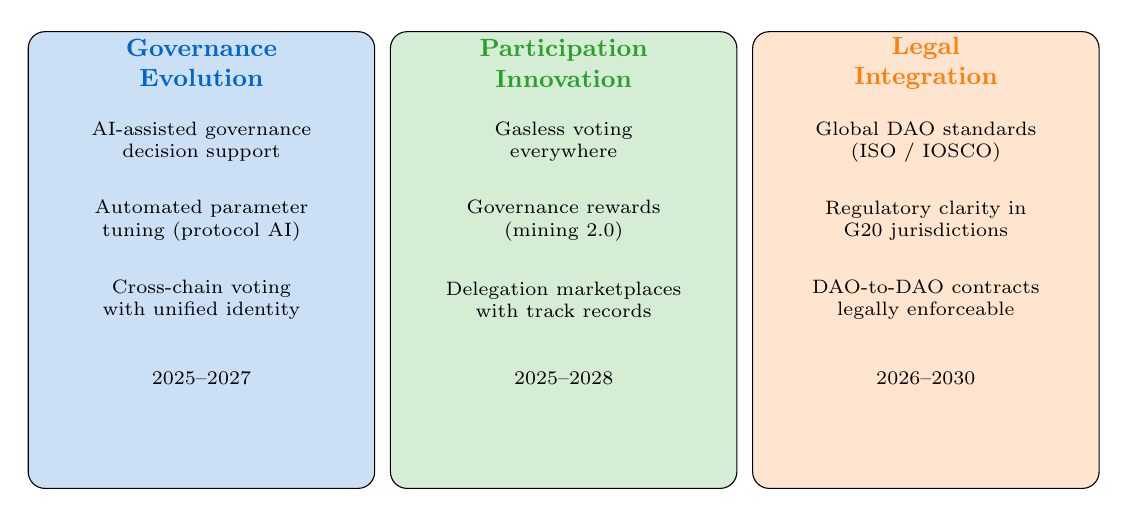
\begin{tikzpicture}
  %% Panel 1: Governance Evolution
  \node[draw,fill=mlblue!20,rounded corners=6pt,
        minimum width=4.4cm,minimum height=5.8cm,align=center,font=\small]
        (p1) at (-4.6,0) {};
  \node[align=center,font=\small\bfseries,text=mlblue] at (-4.6,2.5)
        {Governance\\Evolution};
  \node[align=center,font=\scriptsize] at (-4.6, 1.5)
        {AI-assisted governance\\decision support};
  \node[align=center,font=\scriptsize] at (-4.6, 0.5)
        {Automated parameter\\tuning (protocol AI)};
  \node[align=center,font=\scriptsize] at (-4.6,-0.5)
        {Cross-chain voting\\with unified identity};
  \node[align=center,font=\scriptsize] at (-4.6,-1.5)
        {2025--2027};
  %% Panel 2: Participation Innovation
  \node[draw,fill=mlgreen!20,rounded corners=6pt,
        minimum width=4.4cm,minimum height=5.8cm,align=center,font=\small]
        (p2) at (0,0) {};
  \node[align=center,font=\small\bfseries,text=mlgreen] at (0,2.5)
        {Participation\\Innovation};
  \node[align=center,font=\scriptsize] at (0, 1.5)
        {Gasless voting\\everywhere};
  \node[align=center,font=\scriptsize] at (0, 0.5)
        {Governance rewards\\(mining 2.0)};
  \node[align=center,font=\scriptsize] at (0,-0.5)
        {Delegation marketplaces\\with track records};
  \node[align=center,font=\scriptsize] at (0,-1.5)
        {2025--2028};
  %% Panel 3: Legal Integration
  \node[draw,fill=mlorange!20,rounded corners=6pt,
        minimum width=4.4cm,minimum height=5.8cm,align=center,font=\small]
        (p3) at (4.6,0) {};
  \node[align=center,font=\small\bfseries,text=mlorange] at (4.6,2.5)
        {Legal\\Integration};
  \node[align=center,font=\scriptsize] at (4.6, 1.5)
        {Global DAO standards\\(ISO / IOSCO)};
  \node[align=center,font=\scriptsize] at (4.6, 0.5)
        {Regulatory clarity in\\G20 jurisdictions};
  \node[align=center,font=\scriptsize] at (4.6,-0.5)
        {DAO-to-DAO contracts\\legally enforceable};
  \node[align=center,font=\scriptsize] at (4.6,-1.5)
        {2026--2030};
\end{tikzpicture}
\end{center}
\bottomnote{The future of governance is hybrid: human wisdom + algorithmic efficiency + legal legitimacy | No single solution wins alone}
\end{frame}

% Frame 55: Key Takeaways and Course Summary
\begin{frame}{Key Takeaways and Course Summary}
\begin{center}
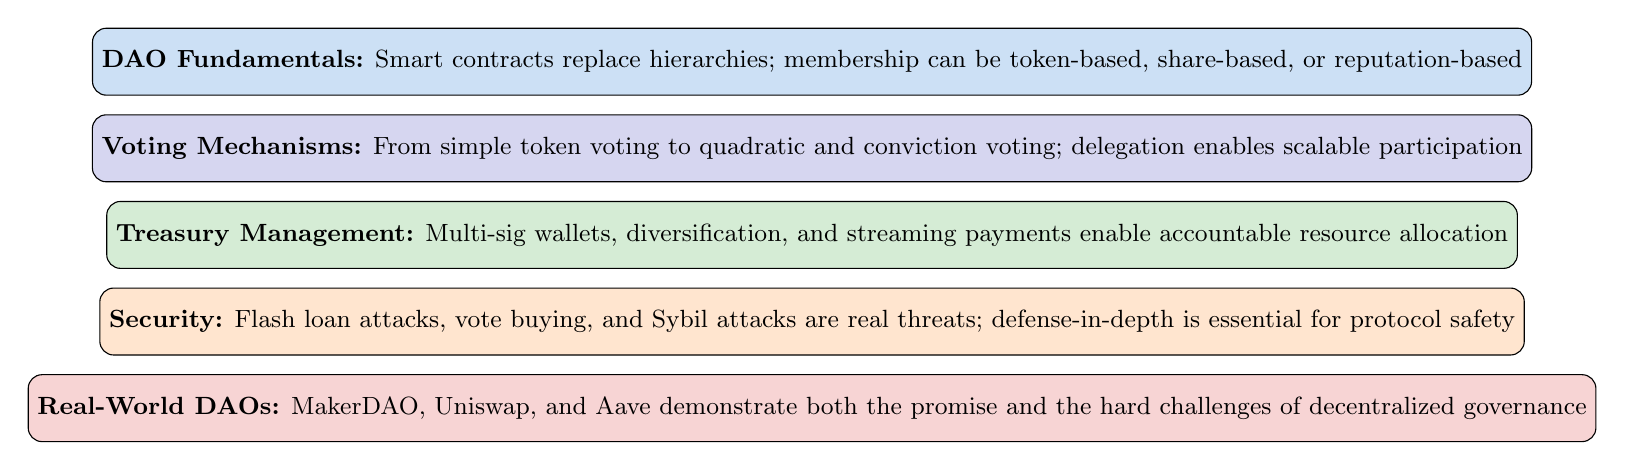
\begin{tikzpicture}
  \node[draw,fill=mlblue!20,rounded corners=5pt,
        minimum width=14.5cm,minimum height=0.85cm,align=center,font=\small]
        at (0, 2.4)
        {\textbf{DAO Fundamentals:} Smart contracts replace hierarchies; membership can be token-based, share-based, or reputation-based};
  \node[draw,fill=mlpurple!20,rounded corners=5pt,
        minimum width=14.5cm,minimum height=0.85cm,align=center,font=\small]
        at (0, 1.3)
        {\textbf{Voting Mechanisms:} From simple token voting to quadratic and conviction voting; delegation enables scalable participation};
  \node[draw,fill=mlgreen!20,rounded corners=5pt,
        minimum width=14.5cm,minimum height=0.85cm,align=center,font=\small]
        at (0, 0.2)
        {\textbf{Treasury Management:} Multi-sig wallets, diversification, and streaming payments enable accountable resource allocation};
  \node[draw,fill=mlorange!20,rounded corners=5pt,
        minimum width=14.5cm,minimum height=0.85cm,align=center,font=\small]
        at (0,-0.9)
        {\textbf{Security:} Flash loan attacks, vote buying, and Sybil attacks are real threats; defense-in-depth is essential for protocol safety};
  \node[draw,fill=mlred!20,rounded corners=5pt,
        minimum width=14.5cm,minimum height=0.85cm,align=center,font=\small]
        at (0,-2.0)
        {\textbf{Real-World DAOs:} MakerDAO, Uniswap, and Aave demonstrate both the promise and the hard challenges of decentralized governance};
\end{tikzpicture}
\vspace{4mm}
\begin{tikzpicture}
  \node[draw,fill=mlpurple,text=white,rounded corners=6pt,
        minimum width=12cm,minimum height=0.8cm,align=center,font=\small\bfseries]
        at (0,0) {Next: Advanced topics in decentralized identity, cross-chain governance, and DAO-to-DAO coordination};
\end{tikzpicture}
\end{center}
\bottomnote{Course complete | DAOs are the organizational frontier of Web3 --- participation, security, and legitimacy remain the defining open challenges}
\end{frame}

\end{document}
